
\chapter{Momento Linear}
\label{Chap:CentroDeMassaEMomentoLinear}

%\minitoc
%\clearpage

% Ver a discussão em https://physics.stackexchange.com/questions/19504/who-discovered-momentum
%
% Aqui seria interessante dar uma nota histórica dizendo que outras pessoas já haviam definido o momento linear, em particular Descartes, que o usou pra estudar colisões.

% Também seria interessante notar que quem deduziu a forma F_R = M a_CM foi o Euler.

\begin{fullwidth}\it
Verificaremos neste capítulo mais algumas consequências das Leis de Newton, apresentando a formulação original para a Segunda Lei de Newton em termos do que chamamos de ``momento linear'', bem como uma forma integral para tal lei. Verificaremos através disso que podemos tratar um sistema de partículas como um só corpo, determinando a posição de seu centro de massa. Finalmente, veremos que sob certas condições o momento linear do sistema é uma constante do movimento, o que nos permite analisar várias situações complexas de maneira relativamente simples.
\end{fullwidth}

%%%%%%%%%%%%%%%%%%%%%%%%
\section{Momento linear}
%%%%%%%%%%%%%%%%%%%%%%%%

Ao estudarmos a Segunda Lei de Newton, utilizamos como variáveis a aceleração e a massa. De acordo com Newton, no entanto,
\begin{quote}
\emph{A alteração do movimento é sempre proporcional à força motriz a ele aplicada; e é feita na direção da linha reta em que tal força atua.}
\end{quote}
%
Na afirmação acima, a palavra \emph{movimento} se refere ao que Newton define como \emph{quantidade de movimento}:
\begin{quote}
\emph{A quantidade de movimento é a medida do mesmo, advindo da velocidade e da quantidade de matéria conjuntamente.}
\end{quote}
%
Matematicamente, temos que tal grandeza, que também é conhecida como \emph{momento linear}, é descrita pela equação
\begin{equation}
    \vec{p} = m \vec{v}.
\end{equation}

Utilizando a definição de momento linear, podemos escrever matematicamente a Segunda Lei de Newton como
\begin{equation}\label{Eq:SegundaLeiMomento}
    \vec{F} = \frac{d\vec{p}}{dt}. \mathnote{Segunda Lei de Newton em termos do momento linear}
\end{equation}
%
Através da definição acima e das propriedades da derivada, podemos escrever
\begin{align}
    \vec{F} &= \frac{dm}{dt}\vec{v} + m\frac{d\vec{v}}{dt} \\
    &= \frac{dm}{dt}\vec{v} + m\vec{a}.
\end{align}
%
Note que se temos uma massa constante, o primeiro termo é zero, restando a conhecida expressão $\vec{F} = m\vec{a}$. No entanto, sistemas com massa variável não são incomuns: um exemplo onde a variação de massa é importante é o caso do lançamento de um foguete, pois tal grandeza varia sensivelmente conforme o combustível é consumido. Não trataremos aqui sistemas onde a massa possa variar, pois estamos tratando somente de corpos rígidos\footnote{Mais do que isso, só tratamos de translações do \emph{centro de massa} de um corpo rígido. Verificaremos como determinar a posição desse ponto nas próximas seções desse capítulo.}, mas uma análise a partir do conceito de momento nos trás resultados bastante interessantes. O principal deles é o surgimento de uma nova lei de conservação, que permitirá uma análise mais simples de diversos problemas.

%%%%%%%%%%%%%%%%%%%%%%%%%%%%%%%%%%%%%%%%%%%%%%%%%%%%%%%%%%%%%%%%%%%%%%%%%%%%%%
\section{Momento linear e Segunda Lei de Newton para um sistema de partículas}
%%%%%%%%%%%%%%%%%%%%%%%%%%%%%%%%%%%%%%%%%%%%%%%%%%%%%%%%%%%%%%%%%%%%%%%%%%%%%%

Nos capítulos anteriores, sempre tratamos os corpos como se eles fossem partículas. Além disso, consideramos que tais partículas ocupavam uma posição específica denominada \emph{centro de massa}. Verificaremos agora por que podemos fazer isso e como devemos proceder para determinar tal posição.

Como vimos anteriormente, um conjunto de partículas interagentes consitui um sistema. Além disso, ao definirmos quais partículas pertencem ao sistema e quais não, definimos automaticamente uma fronteira para o sistema. Vamos nos preocupar agora em definir o momento linear de um sistema de partículas e verificaremos que existe uma forma da Segunda Lei de Newton que se aplica ao sistema como um todo.

Considere um sistema de $N$ partículas interagentes, com massas $m_1$, $m_2$, $m_3$, \dots, $m_N$. Vamos supor que sobre cada partícula $i$ seja exercida uma força resultante $\vec{F}_i^{\rm{Res}}$, de forma que o momento da partícula esteja sujeito a uma variação dada por
\begin{equation}
    \vec{F}_i^{\rm{R}} = \frac{d\vec{p}_i}{dt}.
\end{equation}
%
Podemos escrever a força resultante que atua sobre uma partícula como
\begin{equation}
    \vec{F}_i^{\rm{R}} = \sum \vec{F}_i^{\rm{int}} + \sum \vec{F}_i^{\rm{ext}},
\end{equation}
%
onde $\sum\vec{F}_i^{\rm{int}}$ representa a soma de todas as forças internas do sistema --~isto é, as forças que as partículas do sistema exercem umas sobre as outras~-- e $\sum\vec{F}_i^{\rm{ext}}$ representa a soma de todas as forças externas exercidas sobre a partícula em questão. Assim, podemos escrever
\begin{equation}
    \sum\vec{F}_i^{\rm{int}} + \sum\vec{F}_i^{\rm{ext}} = \frac{d\vec{p}_i}{dt},
\end{equation}
%
ou seja, para cada uma das $N$ partículas temos uma relação com a forma acima:
\begin{align}
    \sum\vec{F}_1^{\rm{int}} + \sum\vec{F}_1^{\rm{ext}} &= \frac{d\vec{p}_1}{dt} \\
    \sum\vec{F}_2^{\rm{int}} + \sum\vec{F}_2^{\rm{ext}} &= \frac{d\vec{p}_2}{dt} \\
    \sum\vec{F}_3^{\rm{int}} + \sum\vec{F}_3^{\rm{ext}} &= \frac{d\vec{p}_3}{dt} \\
    \vdots \\
    \sum\vec{F}_N^{\rm{int}} + \sum\vec{F}_N^{\rm{ext}} &= \frac{d\vec{p}_N}{dt}.
\end{align}
%
Se somarmos todas elas, podemos escrever
\begin{align}
    \sum_{i=1}^N \left[\sum\vec{F}_i^{\rm{int}} + \sum\vec{F}_i^{\rm{ext}}\right] &= \sum_{i=1}^N \frac{d\vec{p}_i}{dt} \\
    \sum_{i=1}^N \sum\vec{F}_i^{\rm{int}} + \sum_{i=1}^N \sum\vec{F}_i^{\rm{ext}} &= \sum_{i=1}^N \frac{d\vec{p}_i}{dt}.
\end{align}
%
O primeiro termo à esquerda representa a soma sobre todas as forças internas. Como tais forças aparecem sempre em pares que ---~devido à Terceira Lei de Newton~--- são iguais em módulo e direção, mas têm sentidos contrários, temos que a soma das forças internas resulta em zero:
\begin{equation}
    \sum_{i=1}^N \vec{F}_i^{\rm{int}} = 0.
\end{equation}
%
O segundo termo à esquerda representa a soma das forças externas, que podemos denominar simplesmente como \emph{força resultante externa}:
\begin{equation}
    \vec{F}_{R}^{\rm{ext}} \equiv \sum_{i=1}^N \vec{F}_i^{\rm{ext}}.
\end{equation}
%
Assim, podemos escrever
\begin{equation}
    \vec{F}_{R}^{\rm{ext}} = \sum_{i=1}^N \frac{d\vec{p}_i}{dt},
\end{equation}
%
ou, sabendo que
\begin{equation}
    \frac{df(x)}{dx} + \frac{dg(x)}{dx} + \frac{dh(x)}{dx} + \dots = \frac{d}{dx} [f(x) + g(x) + g(x) + \dots],
\end{equation}
%
podemos escrever
\begin{equation}
    \vec{F}_{R}^{\rm{ext}} = \frac{d}{dt}\sum_{i=1}^N \vec{p}_i.
\end{equation}

A soma à direita na expressão acima é o vetor resultante da soma de todos os momentos lineares das partículas do sistema --~ou seja, é o \emph{momento linear total do sistema}--, que denotamos por $\vec{P}_{\rm{sis}}$:
\begin{equation}\label{Eq:MomentoLinearSistemaDeParticulas}
    \vec{P}_{\rm{sis}} \equiv \sum_{i=1}^N \vec{p}_i. \mathnote{Momento linear de um sistema de partículas}
\end{equation}
%
Assim, temos
\begin{equation}\label{Eq:SegundaLeiSistemaDeParticulas}
    \vec{F}_{R}^{\rm{ext}} = \frac{d}{dt}\vec{P}_{\rm{sis}}. \mathnote{Segunda Lei de Newton para um sistema de partículas}
\end{equation}
%
Note que o resultado acima para um sistema de partículas é análogo à própria Segunda Lei de Newton para uma partícula, Equação~\eqref{Eq:SegundaLeiMomento}, porém representa a relação entre a variação do momento linear de um sistema como um todo, quando sujeito a forças externas; como visto acima, as forças internas não são capazes de alterar o momento linear total do sistema devido ao fato de que os efeitos das forças do par ação-reação se cancelam. Verificaremos na Seção~\ref{Sec:ConservacaoMomentoLinear} que a equação acima está ligada a uma lei de conservação que será muito importante para analisarmos alguns fenômenos, como por exemplo colisões ou explosões.

%%%%%%%%%%%%%%%%%%%%%%%%%%%%%%%%%%%%%%%
\section{Conservação do momento linear}
\label{Sec:ConservacaoMomentoLinear}
%%%%%%%%%%%%%%%%%%%%%%%%%%%%%%%%%%%%%%%

A partir da Expressão~\eqref{Eq:SegundaLeiSistemaDeParticulas} para a Segunda Lei de Newton, juntamente com a Expressão~\eqref{Eq:MomentoLinearSistemaDeParticulas} para o momento linear de um sistema de partículas, podemos determinar uma \emph{lei de conservação}.

Sabemos que a definição de um sistema é arbitrária. Nesse caso, podemos o escolher de maneira que a \emph{a força resultante externa seja nula}. Nesse caso, temos que o momento linear do sistema de partículas deve se manter constante, já que
\begin{equation}
	\vec{F}_R^{\rm{ext}} = \frac{d}{dt} \vec{P}_{sis}.
\end{equation}
%
Isso significa que \emph{se a força resultante externa é zero, então o momento linear total do sistema se mantém constante, não importando que interações aconteçam entre as partículas}. Consequentemente, entre dois instantes inicial $i$ e final $f$ quaisquer, temos que:
\begin{equation}\label{Eq:ConservacaoMomentoLinear}
	\vec{P}_{\rm{sis}}^i = \vec{P}_{\rm{sis}}^f. \mathnote{Princípio da conservação do momento linear}
\end{equation}

A expressão acima é extremamente relevante pois é muito comum que possamos definir um sistema de maneira que a força resultante externa seja nula. A conservação do momento linear nos fornece um valor cujo cálculo é simples e descreve uma característica do sistema como um todo. Além disso, como o momento linear do sistema é dado pela soma dos momentos lineares das diversas partículas que o compôe, temos uma relação entre os momentos de tais partículas. De uma maneira geral, podemos traçar um paralelo com a conservação da energia, e podemos afirmar que o fato de que o momento linear se conservar nos permite a obtenção de variáveis em um sistema sem a necessidade de entender quais são as minúcias de cada interação entre as partículas do sistema.

Se considerarmos uma situação em que a força externa é nula ---~a explosão de um corpo no espaço, longe de qualquer planeta, por exemplo~---, verificamos através da Expressão~\ref{Eq:ConservacaoMomentoLinear} que o momento linear antes e depois da explosão devem ter o mesmo valor, pois a força resultante externa é nula. Se fixarmos o sistema de referência na posição do próprio projétil, temos que o momento linear inicial é nulo, logo
\begin{align}
    \vec{P}_{\rm{CM}}^i &= \vec{P}_{\rm{CM}}^f \\
    0 &= \vec{P}_{\rm{CM}}^f.
\end{align}
%
Lembrando que podemos separar uma relação vetorial em três eixos, temos que
\begin{equation}
\begin{system}
    p_{1,f}^x + p_{2,f}^x + p_{3,f}^x + \dots &= 0 \\
    p_{1,f}^y + p_{2,f}^y + p_{3,f}^y + \dots &= 0 \\
    p_{1,f}^z + p_{2,f}^z + p_{3,f}^z + \dots &= 0,
\end{system}
\end{equation}
%
onde usamos a Equação~\ref{Eq:MomentoLinearSistemaDeParticulas} para escrever o momento linear do sistema como a soma dos momentos lineares de cada partícula. As equações acima nos dão informações que relacionam os diversos momentos lineares das partículas e, em diversas situações, podemos utilizar tais relações, juntamente com algum conhecimento prévio de algumas variáveis para determinar o valor de outra variável que desejamos conhecer.

Devemos observar que o momento linear e a velocidade são grandezas vetoriais, por isso as velocidades na expressão~\eqref{Eq:ConservacaoMomentoUnidimensional} devem ter sinais apropriados conforme seus sentidos sejam  no sentido positivo ou negativo do eixo de referência adotado. Note que a escolha do sentido positivo é arbitrária, porém uma vez escolhido, devemos escrever as velocidades de maneira coerente. Finalmente, os resultados obtidos para a velocidade poderão ser positivos ou negativos, sendo que valores negativos implicam simplesmente em velocidades no sentido negativo do eixo.

%%%%%%%%%%%%%%%%%%%%%%%%%%%%%%%%%%%%%%%%%%%%%%%%%%%%%%%%
\paragraph{Exemplo: Explosão de um corpo em três partes}
%%%%%%%%%%%%%%%%%%%%%%%%%%%%%%%%%%%%%%%%%%%%%%%%%%%%%%%%

\begin{quote}
    Um objeto inicialmente em repouso sobre uma mesa explode em três partes. As velocidades dos fragmentos imediatamente após a explosão são:
\begin{align}
    \vec{v}_1 &= -\np[m/s]{3.0} \versi\\
    \vec{v}_2 &= \np[m/s]{2.55} \versi + \np[m/s]{0.8} \versj \\
    \vec{v}_3 &= \np[m/s]{0.33} \versi - \np[m/s]{1.2} \versj.
\end{align}
%
Se a massa do fragmento 1 é $m_1 = \np[kg]{0,25}$, quais são as massas dos fragmentos 2 e 3?
\end{quote}

\begin{marginfigure}
\centering
\begin{tikzpicture}[>=Stealth]
    \draw[pattern = north west lines, pattern color = gray, draw = gray] (0,0) circle (0.3);
    \draw[dashdotted] (0,0)++(-0.3,0) -- +(-1.5,0);
    \draw[dashdotted, ->] (0,0) ++(0.3,0) -- +(1.5,0) node[below left]{$x$};
    \draw[dashdotted] (0,0) ++(0,-0.3) -- +(0,-1.5);
    \draw[dashdotted, ->] (0,0) ++(0,0.3) -- +(0,1.5) node[below left]{$y$};
    
    \draw[pattern = north west lines] (-1.2,0) circle (1.8mm);
    \draw[->] (-1.38,0) -- node[above]{$\vec{v}_1$} +(-1,0);
    
    \draw[pattern = north west lines] (17.42:1.07) circle (2.1mm);
    \draw[->] (17.42:1.28) -- node[above]{$\vec{v}_2$} +(17.42:0.89);
    
    \draw[pattern = north west lines] (-74.62:0.5) circle (1.5mm);
    \draw[->] (-74.62:0.65) -- node[right]{$\vec{v}_3$} +(-74.62:0.61);
\end{tikzpicture}
\caption{Explosão de um corpo em três partes.}
\end{marginfigure}

Sabemos que o corpo inicialmente está sobre uma mesa e está em repouso. Nesse caso, sabemos que ele está sujeito a uma força normal e à força peso. No entanto, como não há aceleração no sistema, sabemos que as forças devem estar em equilíbrio. Nesse caso, não há nenhuma força externa resultante atuando sobre o sistema, portanto podemos utilizar a conservação do momento linear:
\begin{equation}
    \vec{P}_{\rm{sis}}^i = \vec{P}_{\rm{sis}}^f.
\end{equation}

\begin{marginfigure}
\centering
\begin{tikzpicture}[>=Stealth,
interface/.style={
        % superfície
        postaction={draw,decorate,decoration={border,angle=-45,
                    amplitude=0.2cm,segment length=2mm}}}
                    ]
                    
    \draw[interface] (-2,0) -- (2,0);
    
    \draw[pattern = north west lines] (-0.5,0) rectangle (0.5,0.5);
    \draw[fill] (0, 0.25) circle (1pt);
    \draw[->, thick] (0, 0.25) --+(0,-1) node[right]{$\vec{P}$};
    \draw[->, thick] (0, 0.5) -- +(0,1) node[right]{$\vec{N}$};
\end{tikzpicture}
\caption{Apesar de termos forças externas atuando sobre o corpo, a força resultante externa é nula. Portanto, temos que o momento linear do sistema se mantém constante.}
\end{marginfigure}

\noindent{}O momento linear inicial do sistema é dado pela soma dos momentos lineares dos fragmentos antes da explosão, porém como todos eles estão parados em relação à mesa, temos que
\begin{equation}
    \sum_j \vec{p}_j^i = 0.
\end{equation}
%
Consequentemente, a soma dos momentos lineares após a explosão também é nula:
\begin{equation}
    \sum_j \vec{p}_j^f = 0.
\end{equation}
%
Separando tal relação em três eixos e considerando que só temos três partículas após a explosão, obtemos
\begin{equation}
\begin{system}
    p_1^x + p_2^x + p_3^x &= 0 \\
    p_1^y + p_2^y + p_3^y &= 0,
\end{system}
\end{equation}
%
ou, utilizando $p_x = m v_x$ e $o_y = mv_y$,
\begin{equation}
\begin{system}
    m_1v_1^x + m_2 v_2^x + m_3 v_3^x &= 0 \\
    m_1v_1^y + m_2 v_2^y + m_3 v_3^y &= 0.
\end{system}
\end{equation}
%
Substituindo os valores das velocidades, obtemos duas equações que envolvem as massas:
\begin{equation}
\begin{system}
    -3 \,m_1 + \np{2.55} \,m_2 + \np{0.33} \,m_3 &= 0 \\
    0 \,m_1 + \np{0.8} \,m_2 - \np{1.2} \,m_3 &= 0,
\end{system}
\end{equation}
%
sendo que as soluções são
\begin{align}
    m_2 &= \np[kg]{0.271} \\
    m_3 &= \np[kg]{0.181}.
\end{align}

%%%%%%%%%%%%%%%%%%%%%%%%%%%%%%%%%%%%%%
\section{Centro de massa}
\label{Sec:CentroDeMassa}
%%%%%%%%%%%%%%%%%%%%%%%%%%%%%%%%%%%%%%

Verificamos na Seção~\ref{Sec:MovimentoRelativo} que a velocidade $\vec{v}_S$ de uma partícula que se desloca em relação a um referêncial $S$ pode ser escrita através de
\begin{equation}
     \vec{v}_S = \vec{v}_{S'} + \vec{v}_{S'S},
\end{equation}
%
onde $v_{S'}$ é a velocidade da partícula em relação a um referencial $S'$ e $v_{S'S}$ é a velocidade do referencial $S'$ em relação ao referencial $S$.

Isso nos permite escrever uma relação entre os momentos lineares do sistema nos dois referenciais:
\begin{align}
    \vec{P}_{sis, S} &= \sum m_i \vec{v}_{i,S} \\
    &= \sum m_i (\vec{v}_{S'} + \vec{v}_{S'S}) \\
    &= \sum m_i \vec{v}_{S'} + \sum m_i \vec{v}_{S'S}.
\end{align}
%
O primeiro termo à direita corresponde à soma dos momentos lineares no referencial $S'$:
\begin{equation}
    \vec{P}_{sis, S'} = \sum m_i \vec{v}_{S'},
\end{equation}
%
ou seja, é o momento linear do sistema em tal referencial. Já o segundo termo, considerando que $\vec{v}_{S'S}$ é igual para todas as partículas, pode ser escrito como
\begin{equation}
    \sum m_i \vec{v}_{S'S} = M \vec{v}_{S'S},
\end{equation}
%
onde a variável $M$ representa a massa total do sistema:
\begin{equation}
    M = \sum m_i.
\end{equation}
%
Assim, podemos escrever
\begin{equation}
    \vec{P}_{sis, S} = \vec{P}_{sis, S'} + M \vec{v}_{S'S}.
\end{equation}

Mesmo para um sistema de partículas que se movam de maneira complexa, como no caso das partículas de um gás, existe um referencial $S'_0$ em específico para o qual o momento linear $\vec{P}_{sis, S'_0}$ do sistema é nulo. Tal sistema é especial pois de certa forma ele descreve o comportamento coletivo das partículas: no caso das partículas do gás, se elas estão dentro de um recipiente fechado, a velocidade do referencial $S'_0$ em relação ao referencial $S$ descreve a velocidade coletiva das partículas (que é a mesma do recipiente), mesmo que as velocidades individuais das partículas sejam diferentes umas das outras. Se usarmos tal referencial no lugar de $S'$, obtemos
\begin{equation}
    \vec{P}_{sis, S} = \vec{P}_{sis, S'_0} + M \vec{v}_{S'_0S},
\end{equation}
%
e, ao substituirmos $\vec{P}_{sis, S'_0}$ por zero, 
\begin{equation}
     \vec{P}_{sis, S} = M \vec{v}_{S'_0S}.
\end{equation}
%
Note que a expressão acima nos permite determinar a velocidade do referencial $S'_0$ em relação ao referencial $S$:
\begin{align}
    \vec{v}_{S'_0S} &= \frac{\vec{P}_{sis, S}}{M} \label{Eq:MomSis} \\
    &= \frac{\sum m_i \vec{v}_{i,S}}{M}. \label{Eq:SomaVelPart}
\end{align}

As expressões acima nos convidam a \emph{definir} uma partícula virtual ---~que denominamos como \emph{Centro de massa}~---, cuja massa é dada pela soma das massas das partículas que formam o sistema e cuja velocidade é dada por $\vec{v}_{S'_0S}$. Podemos considerar que a velocidade $\vec{v}_{S'_0S}$ dada pela Equação~\eqref{Eq:SomaVelPart} pode ser escrita como a derivada de
\begin{equation}\label{Eq:CMConjuntoDeParticulas}
    \vec{r}_{\text{CM}} = \frac{\sum m_i \vec{r}_{i,S}}{M}, \mathnote{Posição do centro de massa de um sistema de partículas}
\end{equation}
%
sendo que tal posição corresponde à posição do centro de massa no referencial $S$. Se a velocidade $\vec{v}_{S'_0S}$ representa uma ``velocidade do sistema'', então a posição do centro de massa representa uma ``posição do sistema''. Adotando essa nova nomenclatura, podemos denotar a velocidade e até mesmo definir uma aceleração do centro de massa:
\begin{align}
    \vec{v}_{\text{CM}} = \frac{d}{dt}\vec{r}_{\text{CM}} &= \frac{\sum m_i \vec{v}_{i,S}}{M} \mathnote{Velocidade do centro de massa de um sistema de partículas} \label{Eq:VelCMPart}\\
    \vec{a}_{\text{CM}} = \frac{d}{dt}\vec{v}_{\text{CM}} &= \frac{\sum m_i \vec{a}_{i,S}}{M}. \mathnote{Aceleração do centro de massa de um sistema de partículas} \label{Eq:AcelCMPart}
\end{align}
%
Note ainda que, através da definição $\vec{v}_{\text{CM}} \equiv \vec{v}_{S'_0S}$  o momento linear do sistema pode ser escrito como
\begin{equation}
    \vec{P}_{sis,S} = M\vec{v}_{\text{CM}},
\end{equation}
%
e por isso também é conhecido como \emph{momento linear do centro de massa}.
    
Veremos nas demais seções desse capítulo que muitas grandezas físicas relativas a um sistema de partículas podem ser determinadas de uma maneira mais simples ao utilizarmos as propriedades do centro de massa. Além disso, muitas vezes é mais fácil analisar um fenômeno se considerarmos que o sistema é substituido por uma partícula cuja massa é igual à massa total do sistema, e que ocupa a posição do centro de massa. Na verdade, estivemos fazendo justamente isso nos capítulos anteriores ao tratarmos a cinemática, a dinâmica, e a energia de partículas.

%%%%%%%%%%%%%%%%%%%%%%%%%%%%%%%%%%%%%%%%%%%%%%%%%%%%%%%%%%%%%%%%%%%%%%%%%%%%%%%%%%%%%%%%%%%%%%%%%%%%%%
\paragraph{Cálculo da posição, velocidade e aceleração do centro de massa de um sistema de partículas}
%%%%%%%%%%%%%%%%%%%%%%%%%%%%%%%%%%%%%%%%%%%%%%%%%%%%%%%%%%%%%%%%%%%%%%%%%%%%%%%%%%%%%%%%%%%%%%%%%%%%%%

Para determinarmos a posição do centro de massa de um sistema de partículas, basta utilizarmos a expressão
\begin{equation}
    \vec{r}_{\rm{CM}} = \frac{1}{M} \sum_{i} m_i \vec{r}_i.
\end{equation}
%
Note que a equação acima pode ser decomposta nos eixos $x$, $y$, e $z$:
\begin{subequations}\label{Eq:CMConjuntoDeParticulasEixos}
\begin{align}
    x_{\rm{CM}} &= \frac{1}{M} \sum_{i} m_i x_i \\
    y_{\rm{CM}} &= \frac{1}{M} \sum_{i} m_i y_i \\
    z_{\rm{CM}} &= \frac{1}{M} \sum_{i} m_i z_i
\end{align}
\end{subequations}

\begin{marginfigure}
\centering
\begin{tikzpicture}[>=Stealth]
    \draw[->] (0,0) -- (0.8,0) (1.2,0) -- (2.8,0) (3.2,0) -- (4,0) node[below left]{$x$};
    \draw[pattern = north west lines] (1,0) circle (2mm);   
    \draw[pattern = north west lines] (3,0) circle (2mm);
    
    \draw[fill = white, draw = black] (2,0) circle (1.5pt) node[below]{CM};
    
\end{tikzpicture}
\caption{O centro de um conjunto de corpos pode estar localizado no espaço entre eles.}
\end{marginfigure}

\noindent{}Veja também que o centro de massa não precisa estar localizado em um ponto que ``pertença'' a um corpo: no caso de duas partículas de mesma massa, por exemplo, separadas por uma distância $d$, a posição do centro de massa é ao longo da reta que une ambas as partículas, a uma distância $d/2$ de cada uma delas. Note ainda que que as demais variáveis cinemáticas, obtidas através das derivadas da equação para a posição $\vec{r}_{\text{CM}}$, também podem ser decompostas nos eixos $x$, $y$, e $z$.

%%%%%%%%%%%%%%%%%%%%%%%%%%%%%%%%%%%%%%%%%%%%%%%%%%%%%%%%%%%%%%%%%%%%%%%%%%%%
\paragraph{Exemplo: Posição do centro de massa de um conjunto de partículas}
%%%%%%%%%%%%%%%%%%%%%%%%%%%%%%%%%%%%%%%%%%%%%%%%%%%%%%%%%%%%%%%%%%%%%%%%%%%%

\begin{quote}
    As partículas mostradas na Figura~\ref{Fig:Ex:CM3Particulas} têm massa $m_1 = m_2 = m$ e $m_3 = 2m$. Se suas posições são
        \begin{align}
            \vec{r}_1 &= \np[m]{1} \, \versi + \np[m]{1} \, \versj \\
            \vec{r}_2 &= \np[m]{1.5} \, \versi + \np[m]{2.5} \, \versj \\
            \vec{r}_3 &= \np[m]{3} \, \versi + \np[m]{2} \, \versj,
        \end{align}
determine a posição do centro de massa do sistema.
\end{quote}

\begin{marginfigure}
\centering
\begin{tikzpicture}[>=Stealth]
    \draw[->] (0,0) -- (4,0) node[below left]{$x$ (m)};
    \draw[->] (0,0) -- (0,3) node[below left]{$y$ (m)};
    
    \draw[pattern = north west lines] (1,1) circle (1mm) node[above left]{$m_1$};
    \draw[pattern = north west lines] (3,2) circle (1.5mm) node[above right]{$m_3$};
    \draw[pattern = north west lines] (1.5,2.5) circle (1mm) node[above left]{$m_2$};
    
\end{tikzpicture}
\caption{Sistema composto por três partículas.\label{Fig:Ex:CM3Particulas}}
\end{marginfigure}

De acordo com as Expressões~\ref{Eq:CMConjuntoDeParticulasEixos}, podemos determinar a posição do centro de massa através de
\begin{align}
    x_{\rm{CM}} &= \frac{1}{M} \sum_{i} m_i x_i \\
    &= \frac{1}{4m} [m\cdot(\np[m]{1}) + m\cdot(\np[m]{1.5}) + 2m\cdot(\np[m]{3})] \\
    &= \frac{1}{4} (\np[m]{8,5}) \\
    &= \np[m]{2,125}.
\end{align}
%
\begin{align}
    y_{\rm{CM}} &= \frac{1}{M} \sum_{i} m_i y_i \\
    &= \frac{1}{4m} [m\cdot(\np[m]{1}) + m\cdot(\np[m]{2.5}) + 2m\cdot(\np[m]{2})] \\
    &= \frac{1}{4} (\np[m]{7,5}) \\
    &= \np[m]{1,875}.
\end{align}
%
Logo,
\begin{equation}
    \vec{r}_{\rm{CM}} = \np[m]{2,125} \, \versi + \np[m]{1,875} \, \versj.
\end{equation}

\begin{marginfigure}[1cm]
\centering
\begin{tikzpicture}[>=Stealth]
    \draw[->] (0,0) -- (4,0) node[below left]{$x$ (m)};
    \draw[->] (0,0) -- (0,3) node[below left]{$y$ (m)};
    
    \draw[pattern = north west lines] (1,1) circle (1mm) node[above left]{$m_1$};
    \draw[pattern = north west lines] (3,2) circle (1.5mm) node[above right]{$m_3$};
    \draw[pattern = north west lines] (1.5,2.5) circle (1mm) node[above left]{$m_2$};
    
    \draw (2.125,1.875) circle (1pt) node[below]{CM};
    
\end{tikzpicture}
\caption{Posição do centro de massa do sistema.\label{Fig:Ex:CM3Particulas_2}}
\end{marginfigure}

%%%%%%%%%%%%%%%%%%%%%%%%%%%%%%%%%%%%%%%%%%%%%%%%%%%%
\paragraph{Exemplo: Velocidade do centro de massa}
%%%%%%%%%%%%%%%%%%%%%%%%%%%%%%%%%%%%%%%%%%%%%%%%%%%%

\begin{quote}
    Suponha que as partículas do exemplo anterior tenham velocidades dadas por
    \begin{align}
        \vec{v}_1 &= \np[m/s]{1,5} \, \versi + \np[m/s]{4,9} \, \versj \\
        \vec{v}_2 &= \np[m/s]{-2.4} \, \versi + \np[m/s]{0,9} \, \versj \\
        \vec{v}_3 &= \np[m/s]{0,45} \, \versi + \np[m/s]{-1,9} \, \versj.
    \end{align}
Determine a velocidade do centro de massa do sistema.
\end{quote}

Usando a Equação~\ref{Eq:VelCMPart}, podemos determinar a velocidade do cento de massa através de
\begin{align}
    v^x_{\rm{CM}} &= \frac{1}{M} \sum_{i} m_i v^x_i \\
    &= \frac{1}{4m} [m\cdot(\np[m/s]{1.5}) + m\cdot(\np[m/s]{-2.4}) + 2m\cdot(\np[m/s]{0,45})] \\
    &= \frac{1}{4} (\np[m/s]{0}) \\
    &= 0.
\end{align}
%
\begin{align}
    v^y_{\rm{CM}} &= \frac{1}{M} \sum_{i} m_i v^y_i \\
    &= \frac{1}{4m} [m\cdot(\np[m/s]{4,9}) + m\cdot(\np[m/s]{0,9}) + 2m\cdot(\np[m/s]{-1.9})] \\
    &= \frac{1}{4} (\np[m/s]{2}) \\
    &= \np[m/s]{0,25}.
\end{align}
%
Assim, obtemos
\begin{equation}
    \vec{v}_{\text{CM}} = \np[m/s]{0,25} \; \versj.
\end{equation}

%%%%%%%%%%%%%%%%%%%%%%%%%%%%%%%%%%%%%%%%%%%%%%%%%%
\paragraph{Exemplo: Aceleração do centro de massa}
%%%%%%%%%%%%%%%%%%%%%%%%%%%%%%%%%%%%%%%%%%%%%%%%%%

\begin{quote}
    Ainda considerando as partículas dos dois exemplos anteriores, determine a aceleração do centro de massa considerando que as acelerações das partículas individualmente sejam dadas por
\begin{align}
    \vec{a}_1 &= \np[m/s]{18} \, \versi + \np[m/s]{22} \, \versj \\
    \vec{a}_2 &= -\np[m/s]{3} \, \versi + \np[m/s]{15} \, \versj \\
    \vec{a}_3 &= \np[m/s]{8,5} \, \versi - \np[m/s]{13,6} \, \versj
\end{align}
\end{quote}

Usando a Equação~\ref{Eq:AcelCMPart}, podemos determinar a velocidade do centro de massa através de
\begin{align}
    v^x_{\rm{CM}} &= \frac{1}{M} \sum_{i} m_i a^x_i \\
    &= \frac{1}{4m} [m\cdot(\np[m/s^s]{18}) + m\cdot(\np[m/s^2]{-3}) + 2m\cdot(\np[m/s^2]{8,5})] \\
    &= \frac{1}{4} (\np[m/s^2]{-32}) \\
    &= \np[m/s^2]{8,0}.
\end{align}
%
\begin{align}
    v^y_{\rm{CM}} &= \frac{1}{M} \sum_{i} m_i a^y_i \\
    &= \frac{1}{4m} [m\cdot(\np[m/s^2]{22}) + m\cdot(\np[m/s^2]{15}) + 2m\cdot(\np[m/s^2]{-13,6})] \\
    &= \frac{1}{4} (\np[m/s^2]{9,8}) \\
    &= \np[m/s^2]{2.45}.
\end{align}
%
Assim, obtemos
\begin{equation}
    \vec{a}_{\text{CM}} = \np[m/s^2]{8,0} \; \versi + \np[m/s^2]{2.45} \;\versj.
\end{equation}


%%%%%%%%%%%%%%%%%%%%%%%%%%%%%%%%%%%%%%%%%%%%%%%%%%%%%%%%%
\subsection{Segunda Lei de Newton para o centro de massa}
%%%%%%%%%%%%%%%%%%%%%%%%%%%%%%%%%%%%%%%%%%%%%%%%%%%%%%%%%

Para um sistema de partículas, a Segunda Lei de Newton é dada por
\begin{equation}
    \vec{F}_{R}^{\rm{ext}} = \frac{d}{dt}\vec{P}_{\rm{sis}}.
\end{equation}
%
Através do conceito de centro de massa, podemos escrever o momento linear do sistema como
\begin{equation}
    \vec{P}_{sis} = M\vec{v}_{\text{CM}}.
\end{equation}
%
Substituindo essa última expressão na anterior, podemos escrever
\begin{equation}
    \vec{F}_{R}^{\rm{ext}} = M\vec{a}_{\text{CM}}.
\end{equation}

\begin{marginfigure}[2cm]
\centering
\begin{tikzpicture}[>=Stealth, scale = 0.9,
     interface/.style={
        % superfície
        postaction={draw,decorate,decoration={border,angle=-45,
                    amplitude=0.2cm,segment length=2mm}}},
    ]
    
    %%
    
    \draw[interface] (-0.3,0) -- (4.7, 0);
    
    \draw[decoration={aspect=0.3, segment length=1.5mm, amplitude=2mm,coil},decorate] (1.6,0.5) -- (2.9,0.5);
    \draw (1.5,0.5) -- (1.6,0.5);
    \draw (2.9,0.5) -- (3,0.5);
    
    \draw[pattern = north west lines, pattern color = gray] (3,0) rectangle (4,1);
    \draw[pattern = north west lines, pattern color = gray] (0.5,0) rectangle (1.5,1);
    
    \draw[->, thick] (-0.3,0.5) -- node[above]{$\vec{F}$} (0.5,0.5);
    
\end{tikzpicture}
\caption{Ao submetermos um sistema como o mostrado na figura a uma força $\vec{F}$, diferentes partes apresentarão diferentes acelerações. Podemos, no entanto, descrever a aceleração \emph{coletiva} do sistema através da aceleração do centro de massa.}
\end{marginfigure}

Esse resultado nos permite descrever um comportamento coletivo de um sistema de partículas mesmo quando tal comportamento não é completamente evidente. Um exemplo de um sistema que apresenta um comportamento complexo, porém que tem um movimento coletivo simples é caso em que temos dois blocos de massa $m$ ligados por uma mola, e que podem deslisar sobre uma superfície sem atrito. Ao exercermos uma força $\vec{F}$ lateral sobre um dos blocos, a aceleração de cada um deles será diferente, variando conforme o estado da compressão/distensão da mola: inicialmente a mola estará relaxada e a aceleração do bloco da esquerda será dada por
\begin{equation}
    a = \frac{F}{m},
\end{equation}
%
enquanto a aceleração do bloco da direita é nula. Conforme a mola for comprimida, a aceleração do bloco da esquerda diminui, enquanto a do bloco da direita aumenta. A diferença entre as acelerações leva também a uma diferença inicial de velocidades dos blocos, o que dá origem a um movimento oscilatório entre eles. Apesar de esse comportamento ser complexo, se nos afastarmos o suficiente do sistema, não conseguimos distinguir o comportamento individual dos blocos, mas somente uma aceleração coletiva\footnote[][-2cm]{Nesse problema, se a força externa dá somente um impulso inicial, é possível escrever a posição dos blocos em relação ao um referencial fixado no centro de massa, obtendo equações relativamente simples. A ideia de descrever o sistema no referencial do centro de massa é bastante frutífera em vários fenômenos.} dada por
\begin{align}
    a &= \frac{F_R^{\rm{ext}}}{2m} \\
    &= \frac{F_R^{\rm{ext}}}{M} \\
    &\equiv a_{\rm{CM}}.
\end{align}

\begin{marginfigure}[2cm]
\centering
\begin{tikzpicture}[>=Stealth, decoration=bumps]
    \draw[->] (0,0) -- (4,0) node[below left]{$x$};
    \draw[->] (0,0) -- (0,2) node[below left]{$y$};
    
    \draw[smooth, samples=1000, domain=0:2.33] plot (\x, {2*\x - 0.6*\x*\x});
    \draw[densely dotted, smooth, samples=1000, domain=2.33:3.33] plot (\x, {2*\x - 0.6*\x*\x});
    
    \coordinate (O) at (0,0);
    \coordinate (A) at (1,0);
    \coordinate (B) at (63.434948823:1);
       
	\draw[->, thick] (0,0) -- (63.43:1.5) node[above]{$\vec{v}_0$};
    \pic [draw, "$\theta$", angle eccentricity=1.5] {angle = A--O--B};

	\draw[decorate] (2.33, 1.4) circle (2mm);
        
\end{tikzpicture}
\caption{Em uma explosão, as forças efetuadas sobre as várias partes do corpo que explode são internas. Nesse caso, o movimento do centro de massa não é afetado.\label{Fig:ExplosaoProjetil}}
\end{marginfigure}

Outro caso em que o movimento do centro de massa é mais simples de se descrever é o das partes de um projétil após sua explosão. Imagine que um projétil seja lançado com velocidade $\vec{v}_0$ fazendo um ângulo $\theta$ com a horizontal, sendo que ele explode antes de tocar o solo. Cada uma das partículas que compunham o projétil serão sujeitas a forças muito intensas durante a explosão, tendo suas trajetórias alteradas. Da mesma maneira que para o lançamento de um corpo rígido, sabemos que a força externa resultante sobre as partículas após a explosão será simplesmente\footnote{Estamos desprezando o efeito da força de arrasto.} a soma da força peso de cada uma delas, o que implica em uma força peso igual àquela do projétil antes da explosão:
\begin{align}
	\vec{F}_{R}^{\rm{ext}} &= \sum_i^N \vec{P}_i \\
		&= \vec{P} \\
		&= M\vec{g}.
\end{align}
%
Logo,
\begin{align}
    M a_{\rm{CM}} &= M g \\
    a_{\rm{CM}} &= g.
\end{align}
%
Como a aceleração do centro de massa é a mesma antes, durante, e depois da explosão, concluímos que \emph{a desintegração do projétil não altera a trajetória do centro de massa}.

%%%%%%%%%%%%%%%%%%%%%%%%%%%%%%%%%%%%%
\subsection{Teorema de Mozzi-Chasles}
\label{Sec:TeoremaDeMozziChasles}
%%%%%%%%%%%%%%%%%%%%%%%%%%%%%%%%%%%%%

\begin{marginfigure}
\centering
\begin{tikzpicture}[>=Stealth]
    
    \draw[dotted, smooth, samples=1000, domain=0:3.33] plot ({1*\x}, {2*\x - 0.6*\x*\x});
    \draw[smooth, samples=1000, domain=0:3.1] plot ({1*\x-0.3*sin(8*\x r)}, {2*\x - 0.6*\x*\x - 0.3*cos(8*\x r)});
    
    \begin{scope}
        \draw [rotate = 90] (-1,-0.1) rectangle (1,0.1);
        \draw[fill] (0,-0.3) circle (0.6pt);
        \draw[fill] (0,0) circle (0.8pt);
    \end{scope}

    \begin{scope}[shift = {(1.25,1.5625)}, rotate = 572.96]
        \draw [rotate = 90, gray] (-1,-0.1) rectangle (1,0.1);
        \draw[fill] (0,-0.285) circle (0.6pt);
        \draw[fill, gray] (0,0) circle (0.8pt);
    \end{scope}
    
    \begin{scope}[shift = {(2.75,0.9625)}, rotate = 1260.51]
        \draw [rotate = 90, gray] (-1,-0.1) rectangle (1,0.1);
        \draw[fill] (0,-0.3) circle (0.6pt);
        \draw[fill,gray] (0,0) circle (0.8pt);
    \end{scope}
        
\end{tikzpicture}
\caption{Quando arremessamos um bastão com uma velocidade de rotação, o movimento efetuado por cada partícula é bastante complexo, porém o centro de massa descreve uma parábola.\label{Fig:BastaoArremessadoGirandoLancObliquo}}
\end{marginfigure}

Devido às rotações, movimentos complexos podem ocorrer mesmo ao considerarmos corpos rígidos. Se arremessarmos um corpo extenso em um lançamento oblíquo, verificaremos que para as diferentes partículas do corpo o movimento é em geral muito mais complexo que uma parábola: temos um movimento em que o corpo gira conforme executa a translação, o que confere a cada partícula do corpo uma posição, velocidade e aceleração diferente. No entanto, como a única força externa exercida sobre o corpo é a força peso, verificamos que a aceleração do centro de massa é dada por
\begin{align}
    a_{\rm{CM}} &= \frac{F_R^{\rm{ext}}}{M} \\
    &= \frac{Mg}{M} \\
    &= g.
\end{align}
%
Note que a força resultante externa é dada pela soma das forças peso das diversas partículas que compõe o corpo:
\begin{align}
    F_R^{\rm{ext}} &= \sum_{i=1}^N P_i \\
    &= \sum_{i=1}^N m_i g \\
    &= \left[\sum_{i=1}^N m_i\right] g \\
    &= M g.
\end{align}
%
O resultado acima para a aceleração do centro de massa mostra que a trajetória $\vec{r}_{\rm{CM}}(t)$ tem a forma de uma parábola.

Apesar de o movimento de cada partícula em separado ser muito complexo em um lançamento como o retratado na Figura~\ref{Fig:BastaoArremessadoGirandoLancObliquo}, eles podem ser descritos como \emph{uma rotação em torno de um eixo que passa pelo centro de massa} associado a \emph{uma translação do centro de massa}. O teorema que garante essa possibilidade é conhecido como \emph{Teorema de Mozzi-Chasles}, ou simplesmente como \emph{Teorema de Chasles}. Sua prova é dada na Seção~\ref{Sec:DeducaoTeoremaDeMozziChasles}, porém exige conhecimentos de Cálculo vetorial. Como verificamos acima, a translação do centro de massa equivale à translação de uma partícula. Já a questão das rotações será tratada nos Capítulos~\ref{Chap:Rotacoes} e~\ref{Chap:MomentoAngular}.

%%%%%%%%%%%%%%%%%%%%%%%%%%%%%%%%%%%%%%%%%%%%%%%%%%%%%%%%%%%%%%%%%%%%%%%%
\section{Determinação da posição do Centro de massa de um corpo extenso}
%%%%%%%%%%%%%%%%%%%%%%%%%%%%%%%%%%%%%%%%%%%%%%%%%%%%%%%%%%%%%%%%%%%%%%%%

No caso de um corpo extenso, não podemos utilizar a Expressão~\eqref{Eq:CMConjuntoDeParticulas} devido a razões práticas: mesmo uma pequena quantidade de matéria é composta por um número extremamente grande de partículas, cujas posições e massas não sabemos precisar com exatidão. Devido a essa dificuldade, vamos analisar algumas outras técnicas que nos permitirão determinar a posição do centro de massa de um corpo extenso.

%%%%%%%%%%%%%%%%%%%%%%%%%%%%%%
\subsection{Corpos simétricos}
%%%%%%%%%%%%%%%%%%%%%%%%%%%%%%

\begin{marginfigure}
\centering
\begin{tikzpicture}
    \draw[pattern = north west lines] (0,0) rectangle (2,2);
    \draw[fill] (1,1) circle (1pt);
    
    \draw[pattern = north west lines] (1,-1.5) circle (1);
    \draw[fill] (1,-1.5) circle (1pt);
\end{tikzpicture}
\caption{Para objetos simétricos, a localização do centro de massa é bastante intuitiva: devido à simetria da distribuição de massa, sabemos que a posição deve ser ``central''. \label{Fig:CMFigurasSimetricas}}
\end{marginfigure}

Muitas vezes podemos encontrar o centro de massa de maneira bastante intuitiva. Na Figura~\ref{Fig:CMFigurasSimetricas} temos duas figuras planas, cujas densidades vamos supor homogêneas. Intuitivamente, podemos afirmar que o centro de massa deve estar localizado nas posições marcadas pelos pontos. Sabemos que, na prática, não podemos ter uma figura realmente plana, pois temos três dimensões, porém podemos considerar que o centro de massa esteja localizado entre as duas faces da figura.

Essa intuição está ligada à própria Equação~\eqref{Eq:CMConjuntoDeParticulas}, que representa uma média ponderada das posições das partículas, e ao fato de que os corpos são simétricos e homogêneos. Podemos verificar matematicamente esse resultado para uma figura plana analisando a Figura~\ref{Fig:CMEixoSimetria}.

Na figura, o eixo $\overline{AB}$ divide o objeto em duas parte simétricas. Vamos assumir que o eixo $y$ tem a mesma orientação que o eixo de simetria. Nesse caso, a contribuição para o cálculo do centro de massa devido a uma região em torno de um ponto $P$ é dada por $x_P m_P$, onde $x_P$ é a distância entre o eixo $y$ e o ponto $P$ e $m_P$ é a massa da região. Se o objeto é simétrico, existe um ponto $P'$ localizado em $x_{P'}$ e com massa $m_{P'}$, cuja contribuição para o centro de massa é $x_{P'}m_{P'}$. Como os pontos se localizam em lados oposto em relação ao eixo de simetria, temos que $x_{P'} = - x_P$. Além disso, se o objeto tem densidade homogênea, temos que $m_P = m_{P'}$. Consequentemente,
%

\begin{marginfigure}
\centering
\begin{tikzpicture}[>=Stealth]
    \draw[pattern = north west lines, pattern color = lightgray] (0,0) -- (2,0) -- (2,-1) -- (1,-1) -- (1,-2) -- (0,-2) -- cycle;
    \draw[dashed, <-] (-0.75, 0.75) node[below left] {$y$} -- (1.75,-1.75);
    \draw[dashed,->] (-1.25, -1.25) -- (1.25,1.25) node[below right] {$x$};
    
    \draw[thick] (-0.25, 0.25) -- (1.25,-1.25);
    \draw[fill] (-0.25,0.25) node[left]{$A$} circle (1pt);
    \draw[fill] (1.25,-1.25) node[right]{$B$} circle (1pt);
    
    \draw[fill, lightgray, draw = black] (0.4,-1.2) coordinate (P) circle (1mm);
    \draw[fill] (P) node[below left] {$P$} circle (0.2mm);
    \draw[fill, lightgray, draw = black] (1.2,-0.4) coordinate (PP) circle (1mm);
    \draw[fill] (PP) node[above right] {$P'$} circle (0.2mm);
    \draw[thick, dotted] (P) -- (PP);
    
\end{tikzpicture}
\caption{Em um objeto simétrico, para cada região com massa $m_P$ em torno de um ponto $P$ existe uma região com massa $m_{P'}$ em torno de um ponto $P$, de forma que as distâncias entre os pontos e o eixo de simetria são iguais. Se o objeto tem densidade homoênea, então $m_P = m_{P'}$. \label{Fig:CMEixoSimetria}}
\end{marginfigure}
%
\begin{align}
  x_\textrm{CM} &= \frac{1}{M} (x_P m_P + x_{P'} m_{P'} + \dots) \\
  &= 0,
\end{align}
%
pois para cada ponto na soma acima, temos um ponto simétrico de forma que a soma total seja nula. Consequentemente, \emph{sempre que houver um eixo de simetria em um corpo com densidade uniforme, sabemos que o centro de massa necessariamente reside sobre tal eixo}. Portanto, a existência de um eixo de simetria simplifica o problema de determinação do centro de massa.

Se pudermos determinar mais que um eixo de simetria, o centro de massa reside sobre o encontro de tais eixos. No caso de uma figura plana, são suficientes dois eixos de simetria diferentes para que possamos determinar exatamente a posição do centro de massa. Na Figura~\ref{Fig:CMQuadrado}, mostramos dois eixos que dividem um quadrado em partes siméticas. Note que esses não são os únicos eixos possíveis: poderíamos utilizar os eixos horizontal e vertical que dividem o quadrado em dois retângulos, ou quaisquer outros eixos que dividam o quadrado em duas partes simétricas.
\begin{marginfigure}[-2cm]
\centering
\begin{tikzpicture}
    \draw[pattern = north west lines, pattern color = lightgray] (0,0) rectangle (2,-2);
    
    \draw[dashed] (-0.5,0.5) -- (2.5,-2.5);
    \draw[dashed] (-0.5,-2.5) -- (2.5,0.5);

    \draw[fill] (1,-1) circle (1.3pt);
\end{tikzpicture}
\caption{Uma placa quadrada e fina pode ser considerada como uma figura plana. Nesse caso, vemos que ela pode ser dividida em partes simétricas através de \emph{eixos de simetria}, sendo que o centro de massa se localiza no encontro de tais eixos. \label{Fig:CMQuadrado}}
\end{marginfigure}


No caso de termos um corpo cujas três dimensões são não desprezíveis, isto é, um corpo que não pode ser interpretado como uma figura plana, podemos utilizar \emph{planos de simetria} para determinar a posição do centro de massa: se existe um plano de simetria, em um argumento idêntico ao do caso bidimensional, verificamos que o centro de massa necessariamente pertence ao plano de simetria. Se existe mais de um plano de simetria, o centro de massa é um ponto que pertence a todos os planos de simetria. Na Figura~\ref{Fig:CMCubo} temos um cubo, onde destacamos três planos que o dividem em partes simétricas. No encontro desses três planos temos um ponto em comum --~que corresponde ao centro de massa~--, marcado como a origem do sistema de coordenadas mostrado. 

\begin{figure}
\centering
\begin{minipage}[c]{0.48\linewidth}
\centering
\begin{tikzpicture}[>=Stealth, rotate around y = -7]

    % eixos
    \draw[->] (0,0,0) -- (1.75,0,0) node[below]{$x$};
    \draw[->] (0,0,0) -- (0,1.75,0) node[left]{$y$};
    \draw[->] (0,0,0) -- (0,0,1.75) node[left]{$z$};
    
    % arestas visíveis
    \draw[thick] (1,1,1) -- (-1,1,1) -- (-1,-1,1) -- (1,-1,1) -- cycle;
    \draw[thick] (1,1,1) -- (1,1,-1) -- (-1,1,-1) -- (-1,1,1);
    \draw[thick] (1,-1,1) -- (1,-1,-1) -- (1,1,-1);
    
    % arestas ocultas
    \draw[dashed] (-1,-1,-1) -- (-1,-1,1);
    \draw[dashed] (-1,-1,-1) -- (1,-1,-1);
    \draw[dashed] (-1,-1,-1) -- (-1,1,-1);
    
    % pontos de interseção dos eixos com as faces
    \draw[fill] (1,0,0) circle (0.5pt);
    \draw[fill] (0,1,0) circle (0.5pt);
    \draw[fill] (0,0,1) circle (0.5pt);
    
    % planos
    % xy
    \draw[densely dotted] (1,1,0) -- (-1,1,0) -- (-1,-1,0) -- (1,-1,0) -- cycle;
    % xz
    \draw[densely dotted] (1,0,1) -- (-1,0,1) -- (-1,0, -1) -- (1,0,-1) -- cycle;
    % yz
    \draw[densely dotted] (0,1,1) -- (0,-1,1) -- (0,-1,-1) -- (0,1,-1) -- cycle;
    
    % centro de massa
    \draw[fill] (0,0,0) circle (1pt);
    
\end{tikzpicture}
\end{minipage}
%
\begin{minipage}[c]{0.48\linewidth}
\centering
\begin{tikzpicture}[>=Stealth, rotate around y = -3]

    % eixos
    \draw[->] (0,0,0) -- (1.75,0,0) node[below]{$x$};
    \draw[->] (0,0,0) -- (0,1.75,0) node[left]{$y$};
    \draw[->] (0,0,0) -- (0,0,1.75) node[left]{$z$};
    
    % arestas visíveis
    \draw[thick] (1,1,1) -- (-1,1,1) -- (-1,-1,1) -- (1,-1,1) -- cycle;
    \draw[thick] (1,1,1) -- (1,1,-1) -- (-1,1,-1) -- (-1,1,1);
    \draw[thick] (1,-1,1) -- (1,-1,-1) -- (1,1,-1);
    
    % arestas ocultas
    \draw[dashed] (-1,-1,-1) -- (-1,-1,1);
    \draw[dashed] (-1,-1,-1) -- (1,-1,-1);
    \draw[dashed] (-1,-1,-1) -- (-1,1,-1);
    
    % pontos de interseção dos eixos com as faces
    \draw[fill] (1,0,0) circle (0.5pt);
    \draw[fill] (0,1,0) circle (0.5pt);
    \draw[fill] (0,0,1) circle (0.5pt);
    
    % planos
    % xy
    \draw[densely dotted] (1,1,0) -- (-1,1,0) -- (-1,-1,0) -- (1,-1,0) -- cycle;
    % xz
    \draw[densely dotted] (1,0,1) -- (-1,0,1) -- (-1,0, -1) -- (1,0,-1) -- cycle;
    % yz
    \draw[densely dotted] (0,1,1) -- (0,-1,1) -- (0,-1,-1) -- (0,1,-1) -- cycle;
    
    % centro de massa
    \draw[fill] (0,0,0) circle (1pt);
    
\end{tikzpicture}
\end{minipage}
\caption{\emph{Figura estereoscópica:} No caso de um cubo, devemos encontrar três planos que o dividem em partes simétricas. A figura acima mostra três possíveis planos dentre os diversos que são capazes de dividir o cubo simetricamente. \label{Fig:CMCubo}}
\end{figure}

%%%%%%%%%%%%%%%%%%%%%%%%%%%%%%%%%%%%%%%%%%%%%%%%%%%%%%%
\subsection{Centro de massa de um objeto discretizável}
%%%%%%%%%%%%%%%%%%%%%%%%%%%%%%%%%%%%%%%%%%%%%%%%%%%%%%%

Em muitos casos não é possível determinar eixos de simetria para um corpo, ou --~se pudermos~-- não conseguimos determinar eixos suficientes para determinar exatamente a posição do centro de massa. Nesse caso, podemos unir as observações sobre simetria e a Equação~\ref{Eq:CMConjuntoDeParticulas} para o centro de massa de um conjunto de partículas para criar um novo método para a determinação do centro de massa.

\begin{marginfigure}
\centering
\begin{tikzpicture}[>=Stealth]

    \draw[pattern = north west lines] (0,0) -- (3,0) -- (3,-1) -- (2, -1) -- (2,-2) -- (4, -2) -- (4,-3) -- (0,-3) -- cycle;

\end{tikzpicture}
\caption{Exemplo de uma figura que não pode ser dividida em duas partes simétricas. \label{Fig:PlacaAssimetrica}}
\end{marginfigure}

Verificamos que a Equação~\ref{Eq:CMConjuntoDeParticulas} é dada por uma soma sobre todas as partículas de um sistema. Se tomarmos uma placa como a da Figura~\ref{Fig:PlacaAssimetrica}, a princípio poderíamos somar sobre todas as partículas que a compõe e determinar a posição do centro de massa. Para efetuar essa soma, vamos dividir as partículas em três regiões, mostradas na Figura~\ref{Fig:PlacaAssimetricaDividida}. Podemos então escrever
\begin{align}
    \vec{r}_{\rm{CM}} &= \frac{1}{M} \sum_{i} m_i \vec{r}_i \\
    &= \frac{1}{M} \left[ \sum_{i}^{R_1} m_i \vec{r}_i + \sum_{i}^{R_2} m_i \vec{r}_i +\sum_{i}^{R_3} m_i \vec{r}_i\right], \label{Eq:Discretizando}
\end{align}
%
onde separamos as partículas de cada região em três somas distintas.

\begin{marginfigure}
\centering
\begin{tikzpicture}[>=Stealth]

    \draw[pattern = north west lines, pattern color = lightgray] (0,0) -- (3,0) -- (3,-1) -- (2, -1) -- (2,-2) -- (4, -2) -- (4,-3) -- (0,-3) -- cycle;
    
    \draw (2,0) -- (2,-3);
    
    \node[fill = white, draw, circle, scale = 0.6] (R1) at (0.25,-0.25) {$1$};
    \node[fill = white, draw, circle, scale = 0.6] (R2) at (2.25,-0.25) {$2$};
    \node[fill = white, draw, circle, scale = 0.6] (R3) at (2.25,-2.25) {$3$};
    
    \draw[dashed,->] (0,-3.3) -- (0, 0.5) node[below left]{$y$};
    \draw[dashed,->] (-0.3,-3) -- (4.5,-3) node[below left]{$x$};
    
    \draw[fill] (1, -1.5) circle (1pt);
    \draw[fill] (2.5,-0.5) circle (1pt);
    \draw[fill] (3, -2.5) circle (1pt);
    
    \draw[dashdotted] (1,0) -- (1,-3);
    \draw[dashdotted] (0,-1.5) -- (2,-1.5);
    
    \draw[dashdotted] (2.5,0) -- (2.5, -1);
    \draw[dashdotted] (2, -0.5) -- (3, -0.5);
    
    \draw[dashdotted] (2,-2.5) -- (4, -2.5);
    \draw[dashdotted] (3,-2) -- (3,-3);

\end{tikzpicture}
\caption{Podemos dividir uma figura em diversas partes para determinar o centro de massa da figura original. Note que o centro de massa de cada região pode ser determinado considerando a simetria de cada divisão.\label{Fig:PlacaAssimetricaDividida}}
\end{marginfigure}

Por outro lado, se tomarmos somente uma das regiões --~ou seja, se destacarmos tal região fazendo um corte na figura~-- podemos determinar o centro de massa de tal região através de
\begin{equation}
    \vec{r}_{\rm{CM}}^{R_j} = \frac{1}{M_{R_j}} \sum_{i}^{R_j} m_i \vec{r}_i,
\end{equation}
%
o que nos dá
\begin{equation}\label{Eq:RegiaoDiscreta}
    \sum_{i}^{R_j} m_i \vec{r}_i = M_{R_j} \vec{r}_{\rm{CM}}^{R_j},
\end{equation}
%
onde usamos o índice $j$ para denotar qualquer uma das regiões e $M_{R_j}$ corresponde à massa de tal região. Podemos utilizar a equação acima para reescrever a equação~\eqref{Eq:Discretizando}, obtendo
\begin{align}
    \vec{r}_{\rm{CM}} &= \frac{1}{M} [M_{R_1} \vec{r}_{\rm{CM}}^{R_1} + M_{R_2} \vec{r}_{\rm{CM}}^{R_2} + M_{R_3} \vec{r}_{\rm{CM}}^{R_3}] \\
    &= \frac{1}{M} \sum_{i} M_{R_i} \vec{r}_{\rm{CM}}^{R_i} \label{Eq:Discretizado}.
\end{align}

O resultado acima mostra que podemos dividir um objeto qualquer em partes menores e determinar a massa e a posição do centro de massa de cada uma dessas regiões. A partir dessas informações, podemos determinar a posição do centro de massa do corpo como um todo utilizando a expresão para o centro de massa de um sistema de partículas. Tal processo equivale a dividir o corpo original em partes menores, substituir tais partes por partículas em seus respectivos centros de massa, e então calcular o centro de massa de tais partículas.

A escolha de como dividir o corpo original é livre, mas para que possamos determinar o centro de massa facilmente, devemos escolher divisões com formas simétricas. Assim, eliminamos a necessidade de realizar a soma contida na equação~\eqref{Eq:RegiaoDiscreta}: basta determinar a posição do centro de massa através de dois ou mais eixos de simetria.

Caso tenhamos um objeto em que as três dimensões são relevantes, podemos generalizar o raciocínio utilizado acima para dividir as partículas em volumes distintos, realizando a soma sobre cada volume. Nesse caso, determinamos centros de massa para cada volume e a partir deles, num raciocínio análogo ao desenvolvido acima para o caso bidimensional, podemos determinar o centro de massa do corpo como um todo através da expressão para o centro de massa para um sistema de partículas. Para determinar a posição do centro de massa de cada um dos volumes, devemos nos valer da liberdade que temos em escolher como dividir o corpo, e das técnicas de simetria da seção anterior --~que no caso tridimensional implica que devemos procurar subdivisões dos corpos que possuam planos de simetria~--.

%%%%%%%%%%%%%%%%%%%%%%%%%%%%%%%
\paragraph{Densidades de massa}
%%%%%%%%%%%%%%%%%%%%%%%%%%%%%%%

É muito comum que ao calcular o centro de massa de um objeto, consideremos que sua densidade é uniforme. Um corpo construído inteiramente do mesmo material, por exemplo, tem densidade uniforme. Nesse caso, é bastante útil descrevermos a massa em termos da densidade do corpo, pois isso possibilita descrever a posição do centro de massa de um ponto de vista puramente geométrico.

Considerando a \emph{densidade volumétrica de massa} $\rho$, definida como
\begin{equation}
    \rho = \frac{M}{V},
\end{equation}
%
temos que a massa $m_i$ de uma parte qualquer do corpo --~se a densidade é uniforme~-- pode ser calculada através
\begin{equation}
    M_i = \rho V_i,
\end{equation}
%
onde $V_i$ representa o volume da referida parte. Assim, podemos reescrever a Expressão~\eqref{Eq:Discretizado} para a posição do centro de massa de um corpo dividido em um número qualquer de regiões como
\begin{align}
    \vec{r}_{\rm{CM}} &= \frac{1}{M} [M_{R_1} \vec{r}_{\rm{CM}}^{R_1} + M_{R_2} \vec{r}_{\rm{CM}}^{R_2} + M_{R_3} \vec{r}_{\rm{CM}}^{R_3} + \dots] \\
    &= \frac{1}{\rho V} [\rho V_{R_1} \vec{r}_{\rm{CM}}^{R_1} + \rho V_{R_2} \vec{r}_{\rm{CM}}^{R_2} + \rho V_{R_3} \vec{r}_{\rm{CM}}^{R_3} + \dots].
\end{align}
%
Note, no entanto, que a densidade aparece no numerador e no denominador. Logo, temos que a posição do centro de massa é dada por
\begin{equation}\label{Eq:CMDensVolConst}
    \vec{r}_{\rm{CM}} = \frac{1}{V} [V_{R_1} \vec{r}_{\rm{CM}}^{R_1} + V_{R_2} \vec{r}_{\rm{CM}}^{R_2} + V_{R_3} \vec{r}_{\rm{CM}}^{R_3} + \dots].
\end{equation}
%
Verificamos, portanto, que a posição do centro de massa de um corpo homogêneo pode ser determinada simplesmente pelas características geométricas de um corpo.

Em muitos casos uma ou mesmo duas dimensões de um corpo são desprezíveis comparadas às demais: no caso de uma chapa metálica, podemos desprezar a espessura, tratando-a como uma figura plana; Já no caso de uma barra fina e longa, podemos tratá-la como um objeto unidimensional. Nesses casos, ao invés de utilizarmos uma densidade volumétrica de massa, podemos definir as densidades \emph{superficial} $\sigma$ e \emph{linear} $\lambda$ de massa:
\begin{align}
    \sigma &= \frac{M}{A} \\
    \lambda &= \frac{M}{L},
\end{align}
%
onde $A$ e $L$ representam a área e o comprimento do corpo em questão. Utilizando tais expressões, podemos escrever expressões análogas à Equação~\ref{Eq:CMDensVolConst} acima, obtendo
\begin{align}
    \vec{r}_{\rm{CM}} &= \frac{1}{A} [A_{R_1} \vec{r}_{\rm{CM}}^{R_1} + A_{R_2} \vec{r}_{\rm{CM}}^{R_2} + A_{R_3} \vec{r}_{\rm{CM}}^{R_3}] \label{Eq:CMDensSupConst}\\
    \vec{r}_{\rm{CM}} &= \frac{1}{L} [L_{R_1} \vec{r}_{\rm{CM}}^{R_1} + L_{R_2} \vec{r}_{\rm{CM}}^{R_2} + L_{R_3} \vec{r}_{\rm{CM}}^{R_3}].\label{Eq:CMDensLinConst}
\end{align}
%
É importante notar que ao tratar um problema qualquer, devemos verificar qual dos casos discutidos acima é o mais adequado. A seguir exemplificaremos o emprego de cada uma delas.

%%%%%%%%%%%%%%%%%%%%%%%%%%%%%%%%%%%%%%%%%%%%%%%%%%%%%%%%%%%%%%%%%%%%%%%%
\paragraph{Exemplo: Centro de massa de um conjunto de barras homogêneas}
%%%%%%%%%%%%%%%%%%%%%%%%%%%%%%%%%%%%%%%%%%%%%%%%%%%%%%%%%%%%%%%%%%%%%%%%

\begin{marginfigure}[3cm]
\centering
\begin{tikzpicture}[>=Stealth]

    \draw[dashed, ->] (0,0) -- (4,0) node[below left] {$x$};
    \draw[dashed, ->] (0,0) -- (0,3.5) node[below left] {$y$};
    
    \draw[very thick] (0,2) -- (0,0) -- (3,0) -- (3,3);
    
    \draw[|-|] (-0.2,2) -- node[left]{$L_1$} (-0.2,0);
    \draw[|-|] (0,-0.2) -- node[below]{$L_2$} (3,-0.2);
    \draw[|-|] (3.2, 0) -- node[right]{$L_3$} (3.2,3);
    
    \draw[fill] (0,1) circle (1.5pt);
    \draw[fill] (1.5,0) circle (1.5pt);
    \draw[fill] (3,1.5) circle (1.5pt);
    
\end{tikzpicture}
\caption{Visão lateral de um corpo formado por três barras finas. \label{Fig:CMBarrasFinas}}
\end{marginfigure}

\begin{quote}
    Um objeto é formado por três barras finas e homogêneas, soldadas como mostra a Figura~\ref{Fig:CMBarrasFinas}. As dimensões do mostradas são
\begin{align}
    L_1 &= \np[cm]{20} \\
    L_2 &= \np[cm]{30} \\
    L_3 &= \np[cm]{30}.
\end{align}
%
Determine a posição do centro de massa em relação ao sistema de referência indicado.
\end{quote}

Por simetria, sabemos que o centro de massa de cada haste deve estar no ponto que divide cada uma delas em dois segmentos com o mesmo tamanho. Com o auxílio do sistema de coordenadas, verificamos que tais posições são
\begin{align}
    \vec{r}_1 &= \np[cm]{10} \;\versj \\
    \vec{r}_2 &= \np[cm]{15} \;\versi \\
    \vec{r}_3 &= \np[cm]{30} \;\versi + \np[cm]{15} \;\versj.
\end{align}

Para determinarmos o centro de massa do sistema como um todo, basta utilizarmos a Equação~\ref{Eq:CMDensLinConst}:
\begin{align*}
    \vec{r}_{\rm{CM}} &= \frac{1}{L} [L_{R_1} \vec{r}_{\rm{CM}}^{R_1} + L_{R_2} \vec{r}_{\rm{CM}}^{R_2} + L_{R_3} \vec{r}_{\rm{CM}}^{R_3} ] \\
    &= \frac{1}{(\np[cm]{20} + \np[cm]{30} + \np[cm]{30})} \Big[(\np[cm]{20}) (\np[cm]{10} \;\versj) \\ \nonumber
    &\phantom{= \frac{1}{(\np[cm]{20} + \np[cm]{30} + \np[cm]{30})} \Big[}+ (\np[cm]{30}) (\np[cm]{15} \;\versi) \\ \nonumber
    &\phantom{= \frac{1}{(\np[cm]{20} + \np[cm]{30} + \np[cm]{30})} \Big[}+ (\np[cm]{30}) (\np[cm]{30} \;\versi + \np[cm]{15} \;\versj)\Big]\\
    &= \frac{\np[cm^2]{200}\;\versj + \np[cm^2]{450}\;\versi + \np[cm^2]{900}\;\versi + \np[cm^2]{450}\;\versj}{\np[cm]{80}} \\
    &= \frac{(\np[cm^2]{450} + \np[cm^2]{900})\versi + (\np[cm^2]{200} + \np[cm^2]{450})\versj}{\np[cm]{80}} \\
    &= \frac{\np[cm^2]{1350}}{\np[cm]{80}}\versi + \frac{\np[cm^2]{650}}{\np[cm]{80}}\versj.
\end{align*}
%
\begin{marginfigure}[-1cm]
\centering
\begin{tikzpicture}[>=Stealth]

    \draw[dashed, ->] (0,0) -- (4,0) node[below left] {$x$};
    \draw[dashed, ->] (0,0) -- (0,3.5) node[below left] {$y$};
    
    \draw[very thick] (0,2) -- (0,0) -- (3,0) -- (3,3);
    
    \draw[|-|] (-0.2,2) -- node[left]{$L_1$} (-0.2,0);
    \draw[|-|] (0,-0.2) -- node[below]{$L_2$} (3,-0.2);
    \draw[|-|] (3.2, 0) -- node[right]{$L_3$} (3.2,3);
    
    \draw[fill] (0,1) circle (1.5pt);
    \draw[fill] (1.5,0) circle (1.5pt);
    \draw[fill] (3,1.5) circle (1.5pt);
    
    \draw[fill] (1.6875,0.8125) circle (1.5pt) node[below right]{CM};
    
\end{tikzpicture}
\caption{Posição do centro de massa. \label{Fig:CMBarrasFinasComCM}}
\end{marginfigure}
%
Finalmente, temos
\begin{equation}
    \vec{r}_{\rm{CM}} = \np[cm]{16,875}\;\versi + \np[cm]{8,125}\;\versj,
\end{equation}
%
que corresponde à posição mostrada na Figura~\eqref{Fig:CMBarrasFinasComCM}.

%%%%%%%%%%%%%%%%%%%%%%%%%%%%%%%%%%%%%%%%%%%%%%%%%
\paragraph{Exemplo: Centro de massa de uma placa}
%%%%%%%%%%%%%%%%%%%%%%%%%%%%%%%%%%%%%%%%%%%%%%%%%

\begin{marginfigure}[3cm]
\centering
\begin{tikzpicture}[scale = 0.9]

    \draw[pattern = north west lines, pattern color = lightgray] (0,0) -- (3,0) -- (3,-1) -- (2, -1) -- (2,-2) -- (4, -2) -- (4,-3) -- (0,-3) -- cycle;
    
    \draw (2,0) -- (2,-3);
    
    \node[fill = white, draw, circle, scale = 0.6] (R1) at (0.25,-0.25) {$1$};
    \node[fill = white, draw, circle, scale = 0.6] (R2) at (2.25,-0.25) {$2$};
    \node[fill = white, draw, circle, scale = 0.6] (R3) at (2.25,-2.25) {$3$};
    
    \draw[dashed,-Stealth] (0,-3.3) -- (0, 0.8) node[below left]{$y$};
    \draw[dashed,-Stealth] (-0.3,-3) -- (4.7,-3) node[below left]{$x$};
    
    \draw[fill] (1, -1.5) circle (1pt);
    \draw[fill] (2.5,-0.5) circle (1pt);
    \draw[fill] (3, -2.5) circle (1pt);
    
    \draw[dashdotted] (1,0) -- (1,-3);
    \draw[dashdotted] (0,-1.5) -- (2,-1.5);
    
    \draw[dashdotted] (2.5,0) -- (2.5, -1);
    \draw[dashdotted] (2, -0.5) -- (3, -0.5);
    
    \draw[dashdotted] (2,-2.5) -- (4, -2.5);
    \draw[dashdotted] (3,-2) -- (3,-3);
    
    \draw[|<->|] (0,0.2) -- node[above]{$L_1$} (3,0.2);
    \draw[|<->|] (-0.2,0) -- node[left]{$L_2$} (-0.2,-3);
    \draw[|<->|] (3.2, 0) -- node[right]{$L_3$} (3.2, -1);
    \draw[|<->|] (2,-1.2) -- node[below]{$L_4$} (3,-1.2);
    \draw[|<->|] (4.2,-2) -- node[right]{$L_5$} (4.2,-3);
    \draw[|<->|] (0,-3.2) -- node[below]{$L_6$} (4,-3.2);

\end{tikzpicture}
\caption{Assumindo que temos uma placa com densidade homogênea, podemos calcular a posição do centro de massa utilizando unicamente informações acerca de sua geometria.\label{Fig:CMPlacaAssimetricaDividida}}
\end{marginfigure}

Podemos determinar exatamente a posição do centro de massa do corpo representado na Figura~\ref{Fig:PlacaAssimetricaDividida}, bastando para isso que tenhamos as medidas de suas laterais, possibilitando que determinemos tanto a área, quanto a posição do centro de massa de cada região. Assumindo que as medidas são
\begin{align*}
    L_1 &= \np[cm]{30} & L_4 &= \np[cm]{10} \\
    L_2 &= \np[cm]{30} & L_5 &= \np[cm]{10} \\
    L_3 &= \np[cm]{10} & L_6 &= \np[cm]{40},
\end{align*}

\noindent{}sabemos que as áreas são
\begin{align}
    A_1 &= \np[cm^2]{600} \\
    A_2 &= \np[cm^2]{100} \\
    A_3 &= \np[cm^2]{200},
\end{align}
%
e que a área total é de \np[cm^2]{900}.

Devido à simetria das regiões escolhidas, sabemos a posição do centro de massa de cada uma delas:
\begin{align}
    \vec{r}_1 &= \np[cm]{10} \;\versi + \np[cm]{15} \;\versj \\
    \vec{r}_2 &= \np[cm]{25} \;\versi + \np[cm]{25} \;\versj \\
    \vec{r}_3 &= \np[cm]{30} \;\versi + \np[cm]{5} \;\versj.
\end{align}
%

\noindent{}Utilizando a Equação~\eqref{Eq:CMDensSupConst}, podemos determinar a posição do centro de massa:
\begin{align*}
    \vec{r}_{CM} &= \frac{1}{\np[cm^2]{900}} [(\np[cm^2]{600})(\np[cm]{10} \;\versi + \np[cm]{15} \;\versj) \\
    &\phantom{= \frac{1}{\np[cm^2]{900}} [}+ (\np[cm^2]{100})(\np[cm]{25} \;\versi + \np[cm]{25} \;\versj) \\
    &\phantom{= \frac{1}{\np[cm^2]{900}} [}+ (\np[cm^2]{200})(\np[cm]{30} \;\versi + \np[cm]{5} \;\versj)] \\
    &=\frac{1}{\np[cm^2]{900}}[(\np[cm^3]{6000} + \np[cm^3]{2500} + \np[cm^3]{6000})\versi \\
    &\phantom{= \frac{1}{\np[cm^2]{900}} [}+ (\np[cm^3]{9000}+ \np[cm^3]{2500} + \np[cm^3]{1000})\versj] \\
    &=\frac{\np[cm^3]{14500}}{\np[cm^2]{900}} \versi + \frac{\np[cm^3]{12500}}{\np[cm^2]{900}}.
\end{align*}


\begin{marginfigure}[-4cm]
\centering
\begin{tikzpicture}[scale = 0.9]

    \draw[pattern = north west lines, pattern color = lightgray] (0,0) -- (3,0) -- (3,-1) -- (2, -1) -- (2,-2) -- (4, -2) -- (4,-3) -- (0,-3) -- cycle;
    
    \draw (2,0) -- (2,-3);
    
    \node[fill = white, draw, circle, scale = 0.6] (R1) at (0.25,-0.25) {$1$};
    \node[fill = white, draw, circle, scale = 0.6] (R2) at (2.25,-0.25) {$2$};
    \node[fill = white, draw, circle, scale = 0.6] (R3) at (2.25,-2.25) {$3$};
    
    \draw[dashed,-Stealth] (0,-3.3) -- (0, 0.8) node[below left]{$y$};
    \draw[dashed,-Stealth] (-0.3,-3) -- (4.7,-3) node[below left]{$x$};
    
    \draw[fill] (1, -1.5) circle (1pt);
    \draw[fill] (2.5,-0.5) circle (1pt);
    \draw[fill] (3, -2.5) circle (1pt);
    
    \draw[dashdotted] (1,0) -- (1,-3);
    \draw[dashdotted] (0,-1.5) -- (2,-1.5);
    
    \draw[dashdotted] (2.5,0) -- (2.5, -1);
    \draw[dashdotted] (2, -0.5) -- (3, -0.5);
    
    \draw[dashdotted] (2,-2.5) -- (4, -2.5);
    \draw[dashdotted] (3,-2) -- (3,-3);
    
    \draw[|<->|] (0,0.2) -- node[above]{$L_1$} (3,0.2);
    \draw[|<->|] (-0.2,0) -- node[left]{$L_2$} (-0.2,-3);
    \draw[|<->|] (3.2, 0) -- node[right]{$L_3$} (3.2, -1);
    \draw[|<->|] (2,-1.2) -- node[below]{$L_4$} (3,-1.2);
    \draw[|<->|] (4.2,-2) -- node[right]{$L_5$} (4.2,-3);
    \draw[|<->|] (0,-3.2) -- node[below]{$L_6$} (4,-3.2);
    
    \draw[fill] (1.611,1.389) +(0,-3) circle (1pt) node[below]{CM};

\end{tikzpicture}
\caption{Posição do centro de massa.\label{Fig:CMPlacaAssimetricaDivididaCM}}
\end{marginfigure}

\noindent{}Finalmente, temos
\begin{equation}
    \vec{r}_{CM} = \np[cm]{16,11}\;\versi + \np[cm]{13,89}\;\versj.
\end{equation}

%%%%%%%%%%%%%%%%%%%%%%%%%%%%%%%%%%%%%%%%%%%%%%%%
\paragraph{Exemplo: Junção de prismas quadrados}
%%%%%%%%%%%%%%%%%%%%%%%%%%%%%%%%%%%%%%%%%%%%%%%%

\begin{quote}
    Determine a posição do centro de massa do corpo formado pela junção de três prismas quadrados, conforme mostra a Figura~\ref{Fig:CMObj3D}. As dimensões são tais que
\begin{equation}
    L = 3 \ell.
\end{equation}
\end{quote}

Dividindo o corpo em partes e utilizando argumentos de simetria, determinamos que os centros de massa das partes estão localizados nas seguintes posições:
\begin{align}
    \vec{r}_1 &= \nicefrac{\ell}{2}\;\versi + 2\ell\;\versj + \nicefrac{\ell}{2}\;\versk \\
    \vec{r}_2 &= \nicefrac{\ell}{2}\;\versi + \nicefrac{\ell}{2}\;\versj + 2\ell\;\versk \\
    \vec{r}_3 &= \nicefrac{3\ell}{2}\;\versi + \nicefrac{\ell}{2}\;\versj + \nicefrac{\ell}{2}\;\versk.
\end{align}

\begin{marginfigure}[-5cm]
\centering
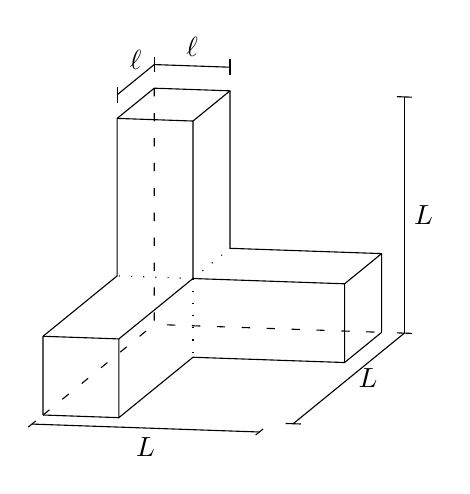
\begin{tikzpicture}[rotate around y = -5]

    % Frente
    \draw (3,0,0) -- (3,1,0) -- (1,1,0) -- (1,3,0) -- (0,3,0);
    \draw (0,3,0) -- (0,3,1) -- (0,1,1) -- (0,1,3) -- (0,0,3);
    \draw (0,3,1) -- (1,3,1) -- (1,1,1) -- (1,1,3) -- (0,1,3);
    \draw (1,1,3) -- (1,0,3) -- (1,0,1) -- (3,0,1) -- (3,0,0);
    \draw (3,0,1) -- (3,1,1) -- (1,1,1);
    \draw (0,0,3) -- (1,0,3);
    \draw (1,3,1) -- (1,3,0);
    \draw (3,1,0) -- (3,1,1);
    
    \draw[loosely dotted] (1,1,1) -- (1,1,0);
    \draw[loosely dotted] (1,1,1) -- (1,0,1);
    \draw[loosely dotted] (1,1,1) -- (0,1,1);
    
    % trás
    \draw[loosely dashed] (0,3,0) -- (0,0,0) -- (3,0,0);
    \draw[loosely dashed] (0,0,3) -- (0,0,0);
    
    % Medidas
    \draw (3.2,0,0) -- (3.4,0,0);
    \draw (3.2,0,3) -- (3.4,0,3);
    \draw (3.3,0,0) -- node[right]{$L$} (3.3,0,3);
    
    \draw (3.3,0,0) -- node[right]{$L$} (3.3,3,0);
    \draw (3.2,3,0) -- (3.4,3,0);
    
    \draw (0,0,3.2) -- (0,0,3.4);
    \draw (3,0,3.2) -- (3,0,3.4);
    \draw (0,0,3.3) -- node[below]{$L$} (3,0,3.3);
    
    \draw (0,3.2,0) -- (0,3.4,0);
    \draw (1,3.2,0) -- (1,3.4,0);
    \draw (0,3.3,0) -- node[above]{$\ell$} (1,3.3,0);
    \draw (0,3.2,1) -- (0,3.4,1);
    \draw (0,3.3,1) -- node[above]{$\ell$}(0,3.3,0);
    
\end{tikzpicture}
\caption{Objeto formado pela junção de três prismas quadrados de comprimento $L$ e laterais $\ell$. As linhas tracejadas representam as arestas na parte de trás do objeto, enquanto as linhas pontilhadas representam as arestas formadas pela inserseção de duas faces dianteiras. \label{Fig:CMObj3D}}
\end{marginfigure}

\begin{marginfigure}
\centering
\begin{tikzpicture}[rotate around x = 15]
    % eixos
    \draw[-Stealth, loosely dashed] (0,0,0) -- (3.5,0,0) node[below left] {$x$};
    \draw[-Stealth, loosely dashed] (0,0,0) -- (0,4,0) node[below left] {$y$};
    \draw[-Stealth, loosely dashed] (0,0,0) -- (0,0,4) node[below right] {$z$};

    % Frente
    \draw (3,0,0) -- (3,1,0) -- (1,1,0) -- (1,3,0) -- (0,3,0);
    \draw (0,3,0) -- (0,3,1) -- (0,1,1) -- (0,1,3) -- (0,0,3);
    \draw (0,3,1) -- (1,3,1) -- (1,1,1) -- (1,1,3) -- (0,1,3);
    \draw (1,1,3) -- (1,0,3) -- (1,0,1) -- (3,0,1) -- (3,0,0);
    \draw (3,0,1) -- (3,1,1) -- (1,1,1);
    \draw (0,0,3) -- (1,0,3);
    \draw (1,3,1) -- (1,3,0);
    \draw (3,1,0) -- (3,1,1);
       
    % planos de simetria e CM
    \draw[dotted] (0,2,0) -- (0,2,1) -- (1,2,1) -- (1,2,0) -- cycle;
    \draw[dotted] (0.5,3,0) -- (0.5,3,1) -- (0.5,1,1) -- (0.5,1,0) -- cycle;
    \draw[dotted] (0,3,0.5) -- (0,1,0.5) -- (1,1,0.5) -- (1,3,0.5) -- cycle;
    \draw[fill] (0.5, 2, 0.5) circle (1pt);
    
%    \draw[dotted] (1.5,0,0) -- (1.5,1,0) -- (1.5,1,1) -- (1.5,0,1) -- cycle;
%    \draw[dotted] (0,0.5,0) -- (3,0.5,0) -- (3,0.5,1) -- (0,0.5,1) -- cycle;
%    \draw[dotted] (0,0,0.5) -- (0,1,0.5) -- (3,1,0.5) -- (3,0,0.5) -- cycle;
    \draw[fill] (1.5,0.5,0.5) circle (1pt);
    
%    \draw[dotted] (0,0,2) -- (0,1,2) -- (1,1,2) -- (1,0,2) -- cycle;
%    \draw[dotted] (0.5,0,1) -- (0.5,1,1) -- (0.5,1,3) -- (0.5,0,3) -- cycle;
%    \draw[dotted] (0,0.5,3) -- (0,0.5,1) -- (1,0.5,1) -- (1,0.5,3) -- cycle;
    \draw[fill] (0.5,0.5,2) circle (1pt);
    
    % cortes
    \draw[dashdotted] (1,1,1) -- (1,1,0) -- (0,1,0) -- (0,1,1) -- cycle;
    \draw[dashdotted] (1,1,1) -- (1,0,1) -- (0,0,1) -- (0,1,1);
    
    % sombra
    \path[pattern = north west lines, pattern color = lightgray] (0,1,0) -- (0,1,1) -- (3,1,1) -- (3,1,0) -- cycle;
    \path[pattern = north east lines, pattern color = lightgray] (0,1,1) -- (0,0,1) -- (3,0,1) -- (3,1,1) -- cycle;
    \path[pattern = north west lines, pattern color = lightgray] (3,1,1) -- (3,0,1) -- (3,0,0) -- (3,1,0) -- cycle;
    
    % rótulos
    \node[draw, circle, scale = 0.7] (P1) at (1,3.3,0) {$1$};
    \node[draw, circle, scale = 0.7] (P2) at (-0.3,1,2.5) {$2$};
    \node[draw, circle, scale = 0.7] (P3) at (2.75,1.3,0) {$3$};
    
\end{tikzpicture}
\caption{Dividimos o objeto em três paralelepípedos, permitindo que determinemos as posições do centro de massa de cada parte através da simetria (para simplificar a figura, mostramos os planos de simetria somente para uma das partes). Verifique que temos um paralelepípedo maior, disposto ao longo do eixo $x$. As linhas ponto-tracejadas mostram os planos de corte para a divisão. \label{Fig:CMObj3DCortado}}
\end{marginfigure}

\noindent{}Os volumes de cada parte são dados por
\begin{align}
    V_1 &= 2\ell^3\\
    V_2 &= 2\ell^3\\
    V_3 &= 3\ell^3,
\end{align}
%
totalizando $7\ell^3$.

Utilizando a Expressão~\eqref{Eq:CMDensVolConst}, podemos determinar a posição do centro de massa:
\begin{align}
    \vec{r}_{CM} &= \frac{1}{7\ell^3} [(2\ell^3)(\nicefrac{\ell}{2}\;\versi + 2\ell\;\versj + \nicefrac{\ell}{2}\;\versk) \\
    &\phantom{=\frac{1}{7\ell^3} [} + (2\ell^3)(\nicefrac{\ell}{2}\;\versi + \nicefrac{\ell}{2}\;\versj + 2\ell\;\versk) \\
    &\phantom{=\frac{1}{7\ell^3} [} + (3\ell^3)(\nicefrac{3\ell}{2}\;\versi + \nicefrac{\ell}{2}\;\versj + \nicefrac{\ell}{2}\;\versk)] \\
    &= \frac{1}{7\ell^3} [(\ell^4 + \ell^4 + \nicefrac{9\ell^4}{2})\versi \\
    &\phantom{=\frac{1}{7\ell^3} [}+ (4\ell^4 + \ell^4 + \nicefrac{3\ell^4}{2})\versj \\
    &\phantom{=\frac{1}{7\ell^3} [}+ (\ell^4 + 4\ell^4 + \nicefrac{3\ell^4}{2})\versk,
\end{align}
%
Finalmente,
\begin{equation}
	\vec{r}_{CM} = \np{0,9286} \ell\; \versi + \np{0,9286} \ell \; \versj + \np{0,9286} \ell \; \versk.
\end{equation}



\noindent{}Observe que o resultado é igual para todos os eixos: existem três planos que são capazes de dividir o corpo em partes simétricas, sendo que o encontro dos três se dá no eixo que passa exatamente no meio do octante formado pelos eixos $x$, $y$ e $z$ --~veja a linha ponto-tracejada na Figura~\ref{Fig:CMObj3DPosicaoCM}~--. Talvez, numa análise instintiva, pudessemos acreditar que o centro de massa estivesse mais afastado da origem, fora do corpo. Uma maneira de perceber o contrário é imaginar um plano a uma altura $y = \ell$: percebemos que a maior parte da massa está abaixo desse plano, portanto o centro de massa também deve estar abaixo do plano. Porém, por simetria, o centro de massa deve estar localizado sobre a reta tracejada. Logo, ele deve estar mais próximo da origem que o ponto $P = \ell \; \versi + \ell \; \versj + \ell \; \versk$ que é a interseção entre o plano $y = \ell$ e a reta. 

\begin{figure}
\centering
\begin{tikzpicture}[rotate around y = 10, rotate around z = -3]
	% eixos
    \draw[-Stealth] (3,0,0) -- (3.5,0,0) node[below left] {$x$};
    \draw[-Stealth] (0,3,0) -- (0,4,0) node[below left] {$y$};
    \draw[-Stealth] (0,0,3) -- (0,0,4) node[below right] {$z$};


    
	% Plano de simetria
	\path[pattern = north west lines, pattern color = lightgray] (0,0,0) -- (0,3.5,0) -- (3,3.5,3) -- (3,0,3) -- cycle;
	\draw[gray] (1,0,1) -- (3,0,3) -- (3,3.5,3) -- (0,3.5,0);

	\draw[pattern = north west lines, pattern color = gray, thick] (0,3,0) -- (1,3,1) -- (0,3,1) -- cycle;
	\draw[pattern = north west lines, pattern color = gray, thick] (1,3,1) -- (0,3,1) -- (0,1,1) -- (1,1,1) -- cycle;
	\draw[pattern = north west lines, pattern color = gray, thick] (1,1,1) -- (0,1,1) -- (0,1,3) -- (1,1,3) -- cycle;
	\draw[pattern = north west lines, pattern color = gray, thick] (0,1,3) -- (1,1,3) -- (1,0,3) -- (0,0,3) -- cycle;
    \draw[pattern = north west lines, pattern color = gray, thick] (1,1,1) -- (1,0,1) -- (1,0,3) -- (1,1,3) -- cycle;

	\draw[pattern = north east lines, pattern color = lightgray] (0,3,0) -- (1,3,0) -- (1,3,1);
	\draw[pattern = north east lines, pattern color = lightgray] (1,3,1) -- (1,3,0) -- (1,1,0) -- (1,1,1) -- cycle;
	\draw[pattern = north east lines, pattern color = lightgray] (1,1,1) -- (1,1,0) -- (3,1,0) -- (3,1,1) -- cycle;
	\draw[pattern = north east lines, pattern color = lightgray] (3,1,0) -- (3,1,1) -- (3,0,1) -- (3,0,0) -- cycle;
	\draw[pattern = north east lines, pattern color = lightgray] (1,1,1) -- (1,0,1) -- (3,0,1) -- (3,1,1) -- cycle;

	\draw[thick] (0,3,0) -- (1,3,1) -- (1,0,1);
	\draw[dashed, thick] (0,0,0) -- (0,3,0);
	\draw[dashed, thick] (0,0,0) -- (0,0,3);
	\draw[dashed, thick] (0,0,0) -- (3,0,0);
	\draw[dashed, thick] (0,0,0) -- (1,0,1);

	\draw[thick, dashdotted] (0,0,0) -- (3,3,3);
	% CM
	\draw[-Stealth, very thick] (0,0,0) -- (0.9286,0.9286,0.9286);
	\draw[fill] (0.9286,0.9286,0.9286) circle (1pt) node[below right]{CM};

\end{tikzpicture}
\caption{Podemos dividir o objeto simetricamente ao realizarmos cortes como o mostrado na figura acima, um para cada eixo. Tais planos determinam uma reta que passa pela origem (reta ponto-tracejada). O vetor denota a posição do centro de massa. \label{Fig:CMObj3DPosicaoCM}}
\end{figure}


%%%%%%%%%%%%%%%%%%%%%%%%%%%%%%%%%%%%%%%%%%%%%%%%%%
\paragraph{Discussão: Determinação da posição do centro de massa por subtração}
%%%%%%%%%%%%%%%%%%%%%%%%%%%%%%%%%%%%%%%%%%%%%%%%%%

Um problema relativamente comum é o de determinar a posição do centro de massa de um corpo com um geometria simples e que tem cavidades também descritas por geometrias simples. A determinação da posição do centro de massa nesses casos é muito complicada se levarmos em conta somente as regiões com massa. Na Figura~\ref{Fig:DetCMPorSubtracao}, por exemplo, temos uma placa quadrada de densidade e espessura uniformes e lado $L$ da qual foi cortada um círculo de raio $L/4$.
\begin{marginfigure}
\centering
\begin{tikzpicture}[>=Stealth]

    \draw[pattern = north west lines] (-2,-2) rectangle (2,2);
    
    \draw[draw = black, fill = white] (1,0) circle (1cm);
    
    \draw[dashed, ->] (-2.5,0) -- (2.5,0) node[below left]{$x$};
    \draw[dashed, ->] (0,-2.5) -- (0,2.5) node[below left]{$y$};


\end{tikzpicture}
\caption{Placa formada pela remoção de um círculo de raio $L/4$ de um quadrado de lado $L$.\label{Fig:DetCMPorSubtracao}}
\end{marginfigure}

Sabemos que se a placa fosse completa, a posição do centro de massa seria a origem do sistema de coordenadas mostrado. Também sabemos que se tomássemos somente o círculo que foi retirado, considerando que ele estivesse em sua posição original, a posição de seu centro de massa seria
\begin{equation}
    \vec{r}_{\text{CM}}^{\bullet} = \frac{L}{4} \versi.
\end{equation}
%
Utilizando a ideia de discretização apresentada anteriormente, podemos considerar o cálculo da posição do centro de massa da placa completa como \emph{a determinação do centro de massa do sistema formado pela região destacada na figura e da parte que foi removida:}
\begin{align}
    \vec{r}_{\text{CM}}^{\blacksquare} &= \frac{1}{M_{\blacksquare}} \sum_i M_{R_i} \vec{r}_{\text{CM}}^{R_i} \\
    &= \frac{1}{M} [M_{\text{placa}} \vec{r}_{\text{CM}}^{\text{placa}} + M_{\bullet} \vec{r}_{\text{CM}}^{\bullet}].
\end{align}
%
A partir da expressão acima, podemos escrever
\begin{align}
    M_{\blacksquare} \vec{r}_{\text{CM}}^{\blacksquare} &= M_{\text{placa}} \vec{r}_{\text{CM}}^{\text{placa}} + M_{\bullet} \vec{r}_{\text{CM}}^{\bullet} \\
    M_{\blacksquare} \vec{r}_{\text{CM}}^{\blacksquare} - M_{\bullet} \vec{r}_{\text{CM}}^{\bullet} &= M_{\text{placa}} \vec{r}_{\text{CM}}^{\text{placa}},
\end{align}
%
de onde obtemos
\begin{equation}
    \vec{r}_{\text{CM}}^{\text{placa}} = \frac{1}{M_{\text{placa}}} [M_{\blacksquare} \vec{r}_{\text{CM}}^{\blacksquare} - M_{\bullet} \vec{r}_{\text{CM}}^{\bullet}].
\end{equation}

Como a placa tem densidade uniforme, podemos reescrever a expressão acima em termos da área como
\begin{align}
    \vec{r}_{\text{CM}}^{\text{placa}} &= \frac{1}{A_{\text{placa}}} [A_{\blacksquare} \vec{r}_{\text{CM}}^{\blacksquare} - A_{\bullet} \vec{r}_{\text{CM}}^{\bullet}] \\
    &= \frac{1}{L^2 - \pi(L/4)^2} [L^2 \vec{r}_{\text{CM}}^{\blacksquare} - \pi\left(\frac{L}{4}\right)^2 \vec{r}_{\text{CM}}^{\bullet}]
\end{align}
%
Como
\begin{align}
    \vec{r}_{\text{CM}}^{\blacksquare} &= 0 \\
    \vec{r}_{\text{CM}}^{\bullet} &= \frac{L}{4} \versi,
\end{align}
%
obtemos
\begin{align}
    \vec{r}_{\text{CM}}^{\text{placa}} &= -\frac{ \pi\left(\frac{L}{4}\right)^2 \frac{L}{4}\versi}{L^2 - \pi(L/4)^2} \\
    &=- \frac{\pi}{4(16-\pi)}L \; \versi.
\end{align}

%%%%%%%%%%%%%%%%%%%%%%%%%%%%%%%%%%%%%%%%%%%%%%%%%%%%%%%%%%%%%%%%%%%%
\subsection{Centro de massa de uma distribuição arbitrária de massa}
%%%%%%%%%%%%%%%%%%%%%%%%%%%%%%%%%%%%%%%%%%%%%%%%%%%%%%%%%%%%%%%%%%%%

A princípio, podemos utilizar a expressão~\eqref{Eq:CMConjuntoDeParticulas} para determinar o centro de massa de qualquer corpo, desde que possamos somar a contribuição de todas as partículas que compõe o corpo. Claramente, no entanto, isso não é nada prático. 

% https://tex.stackexchange.com/questions/123158/tikz-using-the-ellipse-command-with-a-start-and-end-angle-instead-of-an-arc
\tikzset{
    partial ellipse/.style args={#1:#2:#3}{
        insert path={+ (#1:#3) arc (#1:#2:#3)}
    }
}

\begin{marginfigure}[4cm]
\centering
\begin{tikzpicture}[interface/.style={
        % superfície
        postaction={draw,decorate,decoration={border,angle=-45,
                    amplitude=0.2cm,segment length=2mm}}},
    ]

% laterais
\draw (0,0) -- (-1.3,-3);
\draw (1.3,-3) -- (0,0);  

% fundo
\draw[dashed] (-1.28,-3) arc (180:360:1.28 and -0.53);
\draw (-1.3,-3) arc (180:360:1.3 and 0.55);
\draw[fill] (0,-3) circle (0.6pt);

% Eixos
% x
\draw[dotted] (0,-3) -- +(15:-1.15);
\draw[dashdotted,-Stealth] (0,-3) +(15:-1.15) -- +(15:-2) node[below right]{$x$};
\draw[fill](0,-3) +(15:-1.14) circle (0.6pt);
\draw[dotted] (0,-3) -- +(15:1.15);
\draw[dashdotted] (0,-3) +(15:1.15) -- +(15:2);
\draw[fill](0,-3) +(15:1.125) circle (0.6pt);

% y
\draw[dotted] (0,-3) -- +(-15:-1.15);
\draw[dashdotted] (0,-3) +(-15:-1.15) -- +(-15:-2);
\draw[fill](0,-3) +(-15:-1.125) circle (0.6pt);
\draw[dotted] (0,-3) -- +(-15:1.15);
\draw[dashdotted, -Stealth] (0,-3) +(-15:1.15) -- +(-15:2) node[below left]{$y$};
\draw[fill](0,-3) +(-15:1.14) circle (0.6pt);

%
% z
\draw[dashdotted,-Stealth] (0,0) -- (0,0.75) node[below left]{$z$};
\draw[loosely dotted] (0,-3.55) -- (0,0);
\draw[dashdotted] (0,-3.55) -- (0,-4);

\draw[fill] (0,-2.25) circle (1pt) node[above right] {CM};

\begin{scope}[scale = 0.2, shift = {(-2,-12)}]
    \draw[fill, lightgray, draw = black] (1,1,1) -- (1,1,0) -- (0,1,0) -- (0,1,1) -- cycle;
    \draw[fill, lightgray, draw = black] (1,1,1) -- (0,1,1) -- (0,0,1) -- (1,0,1) -- cycle;
    \draw[fill, lightgray, draw = black] (1,1,1) -- (1,1,0) -- (1,0,0) -- (1,0,1) -- cycle;
\end{scope}

\draw[-Stealth] (0,-3) -- node[right]{$\vec{r}_{\rm{CM}}^{R_i}$} (-0.35,-2.38);
\draw[fill] (-0.35,-2.38) circle (0.6pt);

\end{tikzpicture}
\caption{Para determinar a posição do centro de massa de um cone, podemos dividí-lo em diversos cubos e determinar a posição do centro de massa do conjunto de cubos. \label{Fig:CMDiscretizacaoObjeto3D}}
\end{marginfigure}


Se o objeto tem formas complexas, podemos realizar uma divisão em regiões cujos centros de massa possamos determinar por argumentos de simetria, como fizemos nas seções anteriores. Porém, nem sempre uma divisão em cubos é efetiva. Uma maneira alternativa consiste em dividir o corpo em $N$ pequenos cubos contendo diversas partículas, sendo que cada cubo tem massa $M_{R_i}$ ---~como no caso do cone da Figura~\ref{Fig:CMDiscretizacaoObjeto3D}~---. Claramente uma divisão em cubos não é a melhor escolhar para descrever um cone, porém se eles forem pequenos o suficiente, teremos uma aproximação razoável. Esse tipo de procedimento pode ser implementado em programas de computador com certa facilidade, e podem até mesmo considerar situações onde a massa não é homogênea, já que determinamos a massa de cada cubo individualmente.

%\textbf{rever aqui, dar uma olhada num livro de cálculo}
Se tomarmos cubos extremamente pequenos, temos uma soma que tende a infinitos termos. Esse processo é a própria definição de uma uma integral em duas ou três dimensões sobre a área ou volume no qual se distribui a massa:
\begin{align}\label{Eq:CMDistContinua}
  \vec{r}_{\textrm{CM}} &= \lim_{N \to \infty} \frac{1}{M} \sum_{i = 1}^N M_{R_i} \vec{r}_{\rm{CM}}^{R_i} \\
  &= \frac{1}{M} \int \vec{r} \; dm, \mathnote{Centro de Massa de uma distribuição contínua de massa}
\end{align}
%
onde $dm$ representa a massa \emph{infinitesimal} associada a um cubo quando fazemos o número de cubos tendendo ao infinito e $M$ representa a massa total do corpo. Esse resultado pode ser interpretado de uma maneira mais simples se considerarmos que o elemento de massa está relacionado à densidade e ao volume do elemento de massa através de $dm = \rho(\vec{r}) \; dV$. Logo, basta considerarmos uma integral na região do espaço ocupada pelo corpo.

Da mesma forma que na integral em uma dimensão, a ideia não é determinar o resultado desse limite, mas substituir o problema por um equivalente e que nos permita determinar o centro de massa. Matematicamente, o processo de resolução de uma integral em duas ou três dimensões consiste em resolver duas ou três integrais unidimensionais, respectivamente. A principal diferença é a de que os limites de integração não são números, mas funções que descrevem as superfícies externas da região do espaço onde estamos realizando a integração, o que no nosso caso é a própria superfície externa do corpo.


A expressão acima pode ser considerada a forma mais geral de se determinar o centro de massa para uma distribuição contínua de massa, pois a discussão anterior sobre discretização pode ser interpretada como uma simples propriedade da integral acima. Muitas vezes não é necessário considerar o caso tridimensional, bastando substituir $dm = \sigma(\vec{r}) \; dA$ ou $dm = \lambda(x) \; dx$ ---~onde $\sigma(\vec{r})$ e $\lambda(x)$ representam as densidades superficial de massa e a densidade linear de massa (respectivamente), e $dA$ e $dx$ correspondem aos elementos de área e de comprimento~---.

Mesmo assumindo um conhecimento sólido de cálculo, a definição dada pela Equação~\eqref{Eq:CMDistContinua} não é extremamente útil: Precisamos poder descrever a forma do objeto matematicamente, o que só é fácil para formas relativamente simples. De qualquer maneira, para algumas formas (cones e pirâmides, por exemplo) e no caso de termos uma densidade que possa ser calculada para cada ponto do espaço através de uma função, a forma integral é bastante útil.

%%%%%%%%%%%%%%%%%%%%%%%%%%%%%%%%%%%%%%%%%%%%%%%%%%%%%%
\paragraph{Exemplo: Centro de massa de uma barra fina}
%%%%%%%%%%%%%%%%%%%%%%%%%%%%%%%%%%%%%%%%%%%%%%%%%%%%%%

\begin{quote}
    Determine a posição do centro de massa de uma barra fina e homogênea de comprimento $L$ através de uma integral.
\end{quote}

Podemos determinar a posição do centro de massa através da expressão
\begin{align}
    x_{\text{CM}} &= \frac{1}{M} \int x dm \\
    &= \frac{1}{M} \int \lambda x dx,
\end{align}
%
onde assumimos que a barra está disposta de forma que seu eixo aponta na direção do eixo $x$ e usamos $dm = \lambda dx$. Note ainda que a massa $M$ da barra está relacionada à densidade e ao comprimento através de
\begin{equation}
    M = \lambda L.
\end{equation}
%
Se o início da barra coincide com a origem do eixo $x$, então sua extremidade oposta coincide com $x = L$. Logo,
\begin{align}
    x_{\text{CM}} &= \frac{1}{\lambda L} \int_0^L \lambda x dx \\
    &= \frac{\lambda}{\lambda L} \left[\frac{x^2}{2} + C\right]_0^L \\
    &= \frac{1}{L} \left[\left(\frac{L^2}{2} + C\right) - (0 + C)\right] \\
    &= \frac{L}{2}.
\end{align}

%%%%%%%%%%%%%%%%%%%%%%%%%%%%%%%%%%%%%%%%%%%%%%%%%%%%%%%%%%%%%%%%%%%%%%%%%%%%
\paragraph{Exemplo: Centro de massa de uma barra fina de densidade variável}
%%%%%%%%%%%%%%%%%%%%%%%%%%%%%%%%%%%%%%%%%%%%%%%%%%%%%%%%%%%%%%%%%%%%%%%%%%%%

\begin{quote}
    Determine a posição do centro de massa de uma barra fina com densidade linear de massa $\lambda$ variável, dada por
    \begin{equation}
        \lambda = \alpha x,
    \end{equation}
    onde $\alpha$ é uma constante qualquer. Considere que o eixo da barra está alinhado com a direção do eixo $x$, que uma das extremidades da barra se encontra na posição $x = 0$ e que o comprimento total da barra é $L$.
\end{quote}

Podemos determinar a posição do centro de massa através da expressão
\begin{align}
    x_{\text{CM}} &= \frac{1}{M} \int x dm \\
    &= \frac{1}{M} \int \lambda x dx, \\
    &= \frac{1}{M} \int \alpha x^2 dx.
\end{align}
%
Como o início da barra coincide com a origem do eixo $x$, então sua extremidade oposta coincide com $x = L$. Logo,
\begin{align}
    x_{\text{CM}} &= \frac{1}{M} \int_0^L \alpha x^2 dx \\
    &= \frac{\alpha}{M} \left[\frac{x^3}{3} + C\right]_0^L \\
    &= \frac{\alpha}{M} \left[\left(\frac{L^3}{3} + C\right) - (0 + C)\right] \\
    &= \frac{\alpha L^3}{3M}.
\end{align}

Precisamos determinar a massa total da barra, o que pode ser feito através da integral
\begin{align}
    M &= \int dm \\
    &= \int \lambda dx.
\end{align}
%
Como $\lambda = \alpha x$, podemos integrar\footnote{Essa integral pode ser entendida como a soma da massa de várias ``fatias'' da barra. Como a densidade varia, cada fatia tem uma massa diferente, por isso temos que somar desde a menos densa (localizada em $x = 0$), até a mais densa (em $x = L$).} entre $x = 0$ e $x = L$:
\begin{align}
    M &= \int \lambda dx \\
    &= \int_0^L \alpha x dx \\
    &= \alpha \left[\frac{x^2}{2} + C\right]\\
    &= \alpha \left[\left(\frac{L^2}{2} + C\right) - \left(0 + C\right)\right] \\
    &= \alpha \frac{L^2}{2}.
\end{align}

Substituindo o resultado acima para a massa no resultado anterior para a posição do centro de massa, obtemos
\begin{align}
    x_{\text{CM}} &= \frac{\alpha L^3}{3(\alpha L^2 /2)} \\
    &= \frac{2}{3} L.
\end{align}
    
%%%%%%%%%%%%%%%%%%%%%%%%%%%%%%%%%%%%%%%%%%%%%%%%%%%%
%\paragraph{Exemplo: centro de massa de um triângulo}
%%%%%%%%%%%%%%%%%%%%%%%%%%%%%%%%%%%%%%%%%%%%%%%%%%%%
%\textbf{Um que não seja equilátero, óbvio.}

%%%%%%%%%%%%%%%%%%%%%%%%%%%%%%%%%%%%%%%%%%%%%%%
%\paragraph{Exemplo: Centro de massa de um cone}
%%%%%%%%%%%%%%%%%%%%%%%%%%%%%%%%%%%%%%%%%%%%%%%
%\textbf{Ou e um tronco de cone}

%%%%%%%%%%%%%%%%%%%%%%%%%%%%%%%%%%%%%%%%%%%%%%%%%%%%%
\subsection{Centro de massa de um conjunto de corpos}
%%%%%%%%%%%%%%%%%%%%%%%%%%%%%%%%%%%%%%%%%%%%%%%%%%%%%

É relativamente comum que seja necessário determinar o centro de massa de um conjunto de corpos extensos. Nesses casos podemos simplesmente determinar a posição do centro de massa de cada um dos corpos e depois determinar ``o centro de massa dos centros de massa''. Para verificar que isso é verdade, basta utilizarmos o mesmo raciocínio do caso da discretização de um corpo, isto é, devemos dividir a soma sobre o conjunto de partículas que formam o sistema em $n$ somas distintas, onde $n$ é o número de corpos em questão:
\begin{align}
    \vec{r}_{\rm{CM}} &= \frac{1}{M} \sum_{i} m_i \vec{r}_i \\
    &= \frac{1}{M} \left[ \sum_{i}^{C_1} m_i \vec{r}_i + \sum_{i}^{C_2} m_i \vec{r}_i +\sum_{i}^{C_3} m_i \vec{r}_i + \dots\right] \\
    &= \frac{1}{M} \left[ M_{C_1} \vec{r}_{\text{CM}}^{C_1} + M_{C_2} \vec{r}_{\text{CM}}^{C_2} + M_{C_2} \vec{r}_{\text{CM}}^{C_2} + \dots \right] \\
    &= \frac{1}{M} \sum_{j=1}^n M_{C_j} \vec{r}_{\text{CM}}^{C_j}. \label{Eq:CMConjuntoDeCorpos}
\end{align}
%
Assim como no caso da discretização de um corpo, a expressão acima é particularmente útil quando podemos determinar a posição do centro de massa dos corpos por simetria.

%%%%%%%%%%%%%%%%%%%%%%%%%%%%%%%%%%%%%%%%%%%%%%%%%%%%%%%%%
\paragraph{Exemplo: Centro de massa do sistema Terra-Lua}
%%%%%%%%%%%%%%%%%%%%%%%%%%%%%%%%%%%%%%%%%%%%%%%%%%%%%%%%%

\begin{quote}
    Sabendo que a distância entre a Terra e a Lua de é $L = \np[km]{402589}$, que os seus raios são $r_T = \np[km]{6371,0}$ e $r_L = \np[km]{1737,4}$, e supondo que suas densidades são iguais, determine a posição do centro de massa do sistema formado por esses astros. Fixe a origem do sistema de referência no centro da Terra.
\end{quote}

Se considerarmos que ambos os astros são esféricos, podemos determinar a posição do centro de massa através da Equação~\ref{Eq:CMConjuntoDeCorpos} e considerando que $M_i = \rho V_i$:
 \begin{align}
    \vec{r}_{\rm{CM}} &= \frac{1}{\rho(V_T + V_L)} [\rho V_T \vec{r}_{\text{CM}}^T + \rho V_L \vec{r}_{\text{CM}}^L] \\
    &= \frac{1}{(\nicefrac{4}{3}) \pi(r_T^3 + r_L^3)}[(\nicefrac{4}{3})\pi r_T^3 \vec{r}_{\text{CM}}^T + (\nicefrac{4}{3})\pi r_L^3 \vec{r}_{\text{CM}}^L] \\
    &= \frac{1}{r_T^3 + r_L^3} [r_T^3 \vec{r}_{\text{CM}}^T + r_L^3 \vec{r}_{\text{CM}}^L] 
\end{align}
%
No sistema de referência adotados, temos que\footnote{O versor $\hat{r}$ denota um vetor unitário na direção do eixo que liga o centro de massa da Terra ao centro de massa da Lua. Esse versor é usado em coordenadas esféricas.}
\begin{align}
    \vec{r}_{\text{CM}}^T &= 0 \\
    \vec{r}_{\text{CM}}^L &= L \; \hat{r}.
\end{align}
%
Assim,
 \begin{align}
    \vec{r}_{\rm{CM}} &= \frac{1}{r_T^3 + r_L^3} [r_L^3 L \; \hat{r}] \\
    &=\frac{r_L^3}{r_T^3 + r_L^3} L \; \hat{r} \\
    &\approx \np[km]{8002.4}.
\end{align}

%%%%%%%%%%%%%%%%%%%%%%%%%%%%%%%%%%%%%%
\section{Movimento do centro de massa}
%%%%%%%%%%%%%%%%%%%%%%%%%%%%%%%%%%%%%%

Na Seção~\ref{Sec:CentroDeMassa} verificamos que o movimento do centro de massa de um conjunto de partículas só é alterado devido a ação de forças externas, isto é, devido a forças que não são forças de interação entre as partículas que compõe o sistema. Agora que já verificamos como determinar o centro de massa de um corpo e também de um sistema de corpos, podemos analisar alguns sistemas simples que envolvem o movimento do centro de massa.

%%%%%%%%%%%%%%%%%%%%%%%%%%%%%%%%%%%%%%%%%%%%%%%%%%%%%%%%%%%%%%%%%%%%%%%%%
\paragraph{Movimento de corpos de um sistema sujeito à condição de $\vec{F}_R = 0$}
%%%%%%%%%%%%%%%%%%%%%%%%%%%%%%%%%%%%%%%%%%%%%%%%%%%%%%%%%%%%%%%%%%%%%%%%%

Sempre que o sistema estiver sujeito à condição de que $\vec{F}_R = 0$, o movimento do centro de massa deve ser retilíneo e com velocidade uniforme. Isso, porém, não restringe de nenhuma maneira o movimento dos corpos ou partículas que compôe o sistema.

\begin{figure}[b]
\centering
\begin{tikzpicture}[>=Stealth, scale = 0.95,interface/.style={
        % superfície
        postaction={draw,decorate,decoration={border,angle=-45,
                    amplitude=0.2cm,segment length=2mm}}},
    ]

    % Margem
    \draw[interface] (-1.15,0) -- (0,0) -- (0,-1.25);
    
    % Água e tábua
    \draw[decorate, decoration = snake] (0,-0.5) -- (2,-0.5);
    \draw[pattern = north west lines] (2,-0.61) rectangle (9,-0.39);
    \fill (5.5, -0.5) circle (1pt);
    \draw[decorate, decoration = snake] (9,-0.5) -- (10,-0.5);
    
    %% carrinho
    % rodas
    \draw[fill = black] (8.5,-0.25) circle (1.4 mm);
    \draw[fill = black] (7.5,-0.25) circle (1.4 mm);
    \draw[fill = white] (8.5, -0.25) circle (1mm);
    \draw[fill = white] (7.5, -0.25) circle (1mm);
    
    % carroceria
    \draw[fill = gray] (7.1, -0.25) -- (7.3, -0.25) arc[start angle = 180, end angle = 0, radius = 2mm] -- (8.3, -0.25) arc[start angle = 180, end angle = 0, radius = 2mm] -- (9,-0.25) -- (9,0.1) -- (7.7,0.1) -- (7.7,0.7) -- (7.2,0.7) -- (7.1,0.2) -- cycle;
    
    % vidro
    \draw[fill = white] (7.25,0.65) -- (7.65,0.65) -- (7.65, 0.25) -- (7.175, 0.25) -- cycle;
    
    % CM
    \fill (7.9, -0.075) circle (1pt);
    
    % Distâncias
    \draw[dotted] (0,1.5) -- (0,0);
    \draw[dotted] (7.9,1.5) -- (7.9,0.1);
    \draw[|<->|] (0, 1.5) -- node[above]{$\ell$} (7.9,1.5);
    
    \draw[dotted] (5.5,-0.61) -- (5.5,-1);
    \draw[<->|] (0,-1) -- node[below]{$L$} (5.5, -1);
        
\end{tikzpicture}
\caption{Carrinho de brinquedo que se desloca sobre uma tábua que flutua na água. \label{Fig:CanoaSobreAgua}}
\end{figure}

Na Figura~\ref{Fig:CanoaSobreAgua} temos um sistema formado por um carrinho de controle remoto que está sobre uma tábua. A tábua flutua sobre a superfície da água de uma piscina. Inicialmente o sistema se encontra em repouso em relação à margem. A força peso do carrinho e da tábua são equilibradas pela força de empuxo exercida pela água na parte inferior da tábua\footnote{A força peso do carrinho é sustentada diretamente pela força normal exercida pela tábua sobre o carrinho, porém a reação a tal força atua sobre a tábua. Portanto, a força de empuxo deve ser igual à soma dos pesos dos dois corpos, assumindo que o sistema não sofre nenhuma aceleração vertical.}. Quando o carrinho se desloca em direção à margem, a tábua sofre um deslocamento no sentido contrário, no entanto, como as forças de arrasto oferecidas pela água e pelo ar são muito pequenas, podemos considerar que a força resultante externa é nula.

Nesse caso, sabemos que o centro de massa do sistema não está sujeito a nenhuma aceleração, e, como sua velocidade inical em relação à margem é nula, temos que sua posição antes e depois do deslocamento do carrinho são iguais:
\begin{equation}
    x_{\text{CM}}^i = x_{\textrm{CM}}^f.
\end{equation}
%
Como as posições do centro de massa antes ou depois do deslocamento são dadas por
\begin{equation}
    x_{\text{CM}} = \frac{1}{M} [m_c x_{\text{CM}}^{c} + m_t x_{\text{CM}}^t],
\end{equation}
%
podemos escrever
\begin{align}
    x_{\text{CM}}^i &= x_{\textrm{CM}}^f \\
    \frac{1}{M} [m_c x_{\text{CM}}^{c} + m_t x_{\text{CM}}^t] &= \frac{1}{M} [m_c x_{\text{CM}}^{c} + m_t x_{\text{CM}}^t] \\
    m_c \ell^i + m_t L^i &= m_c \ell^f + m_t L^f.
\end{align}
%
A partir da expressão acima, podemos escrever
\begin{equation}
    L^f = \frac{m_c}{m_t}(\ell^i - \ell^f) + L^i.
\end{equation}
%
Note que a distância $L^f$ do centro de massa da tábua até a margem aumenta à medida que $\ell^f$ diminui, isto é, à medida que o carrinho se desloca em direção à margem.

%%%%%%%%%%%%%%%%%%%%%%%%%%%%%%%%%%%%%%%%%%%%%%%%%%%%%%%%%%%%%
\paragraph{Movimentos orbitais dos planetas e seus satélites}
%%%%%%%%%%%%%%%%%%%%%%%%%%%%%%%%%%%%%%%%%%%%%%%%%%%%%%%%%%%%%

Ao contrário da discussão anterior para o carrinho sobre a tábua que flutua, na qual a força resultante externa era nula, no movimento de um planeta juntamente com seus satélites em torno do Sol, temos um sistema onde a força resultante é diferente de zero. Nesse sistema, a força exercida sobre os astros é a força gravitacional do Sol, que faz com que eles orbitem em torno da estrela, sendo que em geral dizemos que a órbita de um planeta é uma elipse em torno do Sol. Essa afirmação, no entanto, é bastante imprecisa.

A solução mais geral para a trajetória de uma partícula sujeita a uma força central é uma \emph{elipse}, sendo que o centro atrator ocupa um dos focos da elipse. A descrição dada acima para o movimento da Terra em torno do Sol não é correta pois ela não executa o movimento em torno do Sol sozinha.

Apesar de aparentemente a Lua orbitar em torno da Terra, o fato é que \emph{ambos} orbitam em torno do centro de massa do sistema Terra-Lua. Isso ocorre pois a Terra também está sujeita a uma força devida à interação gravitacional com a Lua. No entanto, como a posição do centro de massa do sistema Terra-Lua é em um ponto entre o centro e a crosta da Terra, o movimento orbital do planeta é muito menos aparente do que o da Lua\footnote{Imaginando que fosse visto de longe. Existem observações astronômicas de sistemas similares ao Terra-Lua e que apresentam o comportamento descrito.}. Do ponto de vista da interação com o Sol, no entanto, o sistema pode ser tratado como uma partícula, desde que tratemos o movimento do centro de massa. Tal ponto está \emph{aproximadamente} sujeito somente à força central exercida pelo Sol, e executa o movimento elíptico característico de uma órbita.

Em alguns casos, com medidas muito precisas, é possível verificar que os planetas interferem nas órbitas uns dos outros. Netuno e Plutão, por exemplo, foram descobertos a partir de discrepâncias entre os dados experimentais e a trajetória prevista para Urano e Netuno, respectivamente. Mesmo o Sol executa um movimento orbital: de uma maneira geral, todo o sistema solar executa um movimento em torno do centro de massa do sistema como um todo. 

%%%%%%%%%%%%%%%%%%%%%%%%%%%
\paragraph{Salto em altura}
%%%%%%%%%%%%%%%%%%%%%%%%%%%

No salto em altura, o competidor precisa saltar sobre uma barra horizontal disposta a uma altura em relação ao solo. Em nível olímpico, tal altura passa de \np[m]{2,30}. Uma das técnicas que permitem um salto tão alto está relacionada ao centro de massa do corpo do competidor e é conhecida como ``Fosbury Flop'', pois foi introduzida por Dick Fosbury, competidor americano e medalha de ouro no salto em altura em 1968.

A técnica consiste em saltar de costas para a barra, fazendo um arco com o corpo. Isso faz com que o centro de massa seja projetado para fora do corpo do atleta, permitindo que ele passe \emph{sobre} a barra, enquanto o centro de massa passa \emph{sob} ela. Esse processo é vantajoso pois ao saltar, a altura máxima que o centro de massa atinge está limitada pelo impulsionamento inicial dado pelo atleta: até a introdução do ``Forbury Flop'', os atletas saltavam de frente, com o corpo paralelo ao solo, o que os limitava a alturas da barra que fossem menores que a altura máxima atingida pelo centro de massa; após a introdução dessa técnica, para o mesmo impulsionamento inicial, o competidor consegue ``desviar'' o corpo sobre a barra, permitindo que ela seja disposta a alturas maiores.

%%%%%%%%%%%%%%%%%%%%%%%%%%%%%%%%%%%%%%%%%%%%%%%%%%%%%%%%%%%%%%%%%%%%%%%%%
\subsection{Posição do centro de massa e energia potencial gravitacional}
%%%%%%%%%%%%%%%%%%%%%%%%%%%%%%%%%%%%%%%%%%%%%%%%%%%%%%%%%%%%%%%%%%%%%%%%%

Se tomarmos um sistema como o mostrado na Figura~\eqref{Fig:EnergiaPotencialECM}, verificamos que quando a esfera sobre pela pista circular, ela não sofre um deslocamento vertical com o valor do diâmetro da pista, mas sim um deslocamento dado por
\begin{equation}
    \Delta y = 2R - 2r,
\end{equation}
%
onde $R$ é o raio da pista, e $r$ é o raio da esfera. Nessas condições, como podemos determinar a variação da energia potencial gravitacional da esfera?

\begin{marginfigure}
\centering
\begin{tikzpicture}[>=Stealth, interface/.style={
        % superfície
        postaction={draw,decorate,decoration={border,angle=-45,
                    amplitude=0.2cm,segment length=2mm}}},
    ]

    \draw[interface] (60:2) arc[start angle = 60, end angle = 270, radius = 2cm] -- +(2,0);
    \draw[pattern = north west lines] (1,-1.5) circle (0.5);
    \draw[fill] (1,-1.5) circle (0.8pt);
    
    \draw[|-|] (1, -0.5) -- node[above]{$r$} (0.5, -0.5);
    \draw[dotted] (1, -0.5) -- (1,-1);
    \draw[dotted] (0.5, -0.5) -- (0.5,-1.5);
    
    \draw[dashed] (0,1.5) circle (0.5);
    \draw[fill, gray] (0,1.5) circle (0.8pt);
    
    \draw[->] (0.5,-1.5) -- node[above]{$\vec{v}$} +(-0.75,0);
    
    \draw[|-|] (2,-1.5) -- node[right]{$\Delta y$} (2,1.5);
    \draw[dotted] (0.5,1.5) -- (2, 1.5);
    \draw[dotted] (1.5,-1.5) -- (2,-1.5);
    
    \draw[->] (0,0) -- node[below]{$R$} (155:2);
    \draw[fill] (0,0) circle (0.6pt);

\end{tikzpicture}
\caption{Para um corpo rígido, a variação da energia potencial está ligada à variação da posição vertical do centro de massa. Note que no exemplo acima, $\Delta y = 2R - 2r$. \label{Fig:EnergiaPotencialECM}}
\end{marginfigure}

Podemos tratar a esfera como um sistema de partículas, assim, somando as energias potenciais de cada partícula em uma posição qualquer, temos
\begin{equation}
    U_g^{\rm{sis}} = \sum_{i = 1}^N m_i g y_i.
\end{equation}
%
Como a aceleração da gravidade é a mesma para todas as parcelas da soma, podemos tirá-la do somatório, obtendo
\begin{equation}\label{Eq:EnPotGravSisPartSoma}
    U_g^{\rm{sis}} = g \sum_{i = 1}^N m_i y_i.
\end{equation}

Se considerarmos as expressões para a posição do centro de massa nos eixos $x$ e $y$, obtemos
\begin{align}
    x_{\rm{CM}} &= \frac{1}{M} \sum_{i = 1}^N m_i x_ i \\
    y_{\rm{CM}} &= \frac{1}{M} \sum_{i = 1}^N m_i y_ i,
\end{align}
%
ou, para o eixo $y$ em especial,
\begin{equation}
    \sum_{i = 1}^N m_i y_ i = M y_{\rm{CM}}.
\end{equation}
%
Substituindo essa expressão na Equação~\eqref{Eq:EnPotGravSisPartSoma}, obtemos
\begin{equation}
    U_g^{\rm{sis}} = M g y_{\rm{CM}}. \mathnote{Energia potencial gravitacional de um sistema de partículas}
\end{equation}

Constatamos, portanto, que a energia potencial gravitacional de um sistema de partículas é a mesma energia associada a uma partícula de massa $M$, dada pela soma das massas de todas as partículas, e cuja posição vertical é a do próprio centro de massa do sistema. Isso permite que determinemos a variação da energia potencial gravitacional de um corpo simplesmente considerando a variação da posição vertical de seu centro de massa.

%%%%%%%%%%%%%%%%%%%%%%%%%%%%%%%%%%%%%
\paragraph{Exemplo: Bloco em um loop}
%%%%%%%%%%%%%%%%%%%%%%%%%%%%%%%%%%%%%

No capítulo anterior, na página~\pageref{Pag:ExercicioBlocoPistaCircularVertical}, determinamos a compressão necessária de uma mola para que ela armazenasse energia suficiente para que um bloco fosse lançado por uma pista horizontal e chegasse ao topo de uma seção circular da pista. Verificamos que era necessário desprezar as dimensões do bloco, uma vez que não sabíamos determinar a posição do centro de massa. Vamos voltar ao mesmo problema, mas considerando as dimensões dessa vez:
\begin{quote}
    A Figura~\ref{Fig:BlocoArremessadoEmLoop} mostra um bloco \emph{de densidade homogênea, em formato de cubo,} que será lançado, empregando uma mola, em uma pista sem atrito composta de uma seção plana e de uma seção circular vertical. Se a constante elástica da mola é $k = \np[N/m]{1200}$, a massa do bloco é $m = \np[kg]{0.750}$, o raio da pista é $\np[cm]{130}$, \emph{e o cubo tem aresta $L = \np[cm]{30,0}$}, qual deve ser a compressão $\ell$ da mola para que o bloco chegue ao ponto mais alto da pista sem que perca contato com ela, assumindo que ele partiu do repouso?
\end{quote}


\begin{marginfigure}
\centering
\begin{tikzpicture}[>=Stealth, scale = 0.4,
     interface/.style={
        % superfície
        postaction={draw,decorate,decoration={border,angle=-45,
                    amplitude=0.2cm,segment length=2mm}}},
    ]
    
    %%
    
    \draw[interface] (0,-0.5) -- (0,-2.5);
    \draw[interface] (0,-2.5) -- (7.05, -2.5);
    \draw[interface] (7.05,-2.5) arc[start angle = -90, end angle = 123, radius = 3 cm];
    
    \draw[->] (0,-3.2) -- (6.5,-3.2) node[below left]{$x$};
    \draw[|-|] (2.2, -3.2) -- (4.2,-3.2);
    \path (2.2,-3.3) node[below]{$\ell$} -- (4.2,-3.3) node[below]{0};
    
    \draw (0,-2) -- (0.2,-2);
    \draw[decoration={aspect=0.4, segment length=1.5625mm, amplitude=1.6mm,coil},decorate] (0.2,-2) -- (3.3,-2);
    \draw (3.3, -2) -- (3.5,-2);
    
    \draw[pattern = north west lines] (3.7,-2.5) rectangle (4.7,-1.5);
    \draw[pattern = north east lines] (3.5,-2.5) rectangle (3.7,-1.5);
    \draw[<->|] (5,-2.5) -- node[right]{$L$} (5,-1.5);
        
\end{tikzpicture}
\caption{Lançamento de um bloco em uma pista circular vertical.}
\end{marginfigure}

Como havíamos visto, no sistema formado pelo bloco, a mola, e a pista, temos a atuação de três forças: o peso do bloco, a força normal exercida pelas superfícies, e a força exercida pela mola. Dessas, somente a força normal não é conservativa, porém seu trabalho é nulo pois ela atua sempre perpendicularmente ao deslocamento instantâneo do bloco. Portanto, podemos utilizar a conservação da energia mecânica:
\begin{align}
    E_i^{\textrm{mec}} &= E_f^{\textrm{mec}} \\
    K_i + U_e^i + U_g^i &= K_f + U_g^f + U_e^f
\end{align}
%
Como o bloco parte do repouso, sua energia cinética inicial é zero. Vamos escolher a origem do eixo vertical na altura da pista horizontal. Assim, a posição inicial do centro de massa do bloco é
\begin{equation}
    y_{\text{CM}}^i = \frac{L}{2},
\end{equation}
%
uma vez que ele é homogêneo e simétrico. Assim, a expressão acima simplifica-se a:
\begin{equation}\label{Eq:EnergiasParaOBlocoEmLoopCM}
    U_e^i + U_g^i= K_f + U_g^f.
\end{equation}
%
Note que a energia cinética final não é nula, já que o bloco não pode ter velocidade nula ao chegar ao topo da seção circular da pista: 
\begin{equation}
    v = \sqrt{Rg}.
\end{equation}
%
Quando o bloco chega ao topo, a posição vertical final de seu centro de massa será igual ao diâmetro da pista circular, menos a distância entre o centro de massa e a lateral superior do bloco:
\begin{equation}
    y_{\text{CM}}^f = 2R - \frac{L}{2}.
\end{equation}

Substituindo os resultados acima na Equação~\ref{Eq:EnergiasParaOBlocoEmLoopCM} obtemos
\begin{align}
    \frac{kx_i^2}{2} + mgy_{\text{CM}}^i&= \frac{mv_f^2}{2} + mgy_{\text{CM}}^f \\
    \frac{k\ell^2}{2} + mg\frac{L}{2} &= \frac{m(\sqrt{Rg})^2}{2} + mg\left(2R - \frac{L}{2}\right) \\
    \frac{k\ell^2}{2} &= mg\left(2R +\frac{R}{2} - \frac{L}{2} - \frac{L}{2}\right) \\
    k\ell^2 &= 2mg((\nicefrac{5}{2})R - L) \\
    \ell &= \sqrt{\frac{mg(2R - L)}{k}}.
\end{align}
%
Substituindo os valores das constantes, temos finalmente
\begin{align}
    \ell &= \sqrt{2\cdot\frac{(\np[kg]{0.750}) \cdot (\np[m/s^2]{9.8}) \cdot [(\nicefrac{5}{2}) \cdot (\np[m]{1.30}) - (\np[m]{0.30})]}{(\np[N/m]{1200})}} \\
    &\approx \np[m]{0.190}.
\end{align}

%%%%%%%%%%%%%%%%%
\section{Impulso}
%%%%%%%%%%%%%%%%%

A Segunda Lei de Newton na forma dada pela Equação~\eqref{Eq:SegundaLeiMomento} nos dá uma maneira de ligar o valor da força exercida sobre um corpo à variação instantânea do momento linear. Muitas vezes, como no caso de \emph{colisões} entre dois corpos\footnote{Abordaremos colisões na próxima seção.}, estamos interessados em determinar qual é a \emph{variação total} do momento linear. Isso pode ser feito através de uma \emph{integração} da expressão~\eqref{Eq:SegundaLeiMomento}:
\begin{equation*}
    \frac{d\vec{p}}{dt} = \vec{F}(t)
\end{equation*}
%
pois se temos que $\vec{F}(t)$ é a derivada da função $\vec{p}(t)$, então, pelo teorema fundamental do cálculo, a função $\vec{p}(t)$ é a função primitiva/anti-derivada/integral-indefinida de $\vec{F}(t)$ a menos de uma constante $C$:
\begin{equation}
    \vec{p}(t) = \vec{\mathcal{F}}(t) + C.
\end{equation}
%
Como estamos interessados na \emph{variação} do momento linear, tal constante não tem importância:\footnote{Como (quase) sempre.}
\begin{align}
    \Delta \vec{p} &= [\vec{\mathcal{F}}(t_f) + C] - [\vec{\mathcal{F}}(t_i) + C] \\
    &= \int_{t_i}^{t_f} \vec{F}(t) \; dt.\label{Eq:SegundaLeiIntegrando}
\end{align} 
%
A integral à direita na equação acima recebe o nome de \emph{impulso}, e é denotada por $\vec{J}$:
\begin{equation}
    \vec{J} = \int_{t_i}^{t_f} \vec{F}(t) \; dt. \mathnote{Impulso}
\end{equation}
%
Assim, temos que a Segunda Lei de Newton possui uma forma integral, dada por
\begin{equation}\label{Eq:Impulso}
    \Delta \vec{p} = \int_{t_i}^{t_f} \vec{F}(t) \; dt. \mathnote{Segunda Lei de Newton \\ (forma integral)}
\end{equation}

Nos resultados acima, devemos destacar que a força, a variação do momento e o impulso são grandezas vetoriais. Assim, devemos aplicar tais equações a cada eixo separadamente:
\begin{align}
    \Delta p_x &= \int_{t_i}^{t_f} F_x(t) \; dt \\
    \Delta p_y &= \int_{t_i}^{t_f} F_y(t) \; dt \\
    \Delta p_z &= \int_{t_i}^{t_f} F_z(t) \; dt.
\end{align}
%
No entanto, uma escolha adequada do sistema de referências muitas vezes implicará na ausência de componentes de uma força em um ou mais eixos, levando a uma variação nula da componente correspondente do impulso e do momento linear.

\begin{marginfigure}[-5cm]
\centering
\begin{tikzpicture}[>=Stealth, extended line/.style={shorten >=-#1,shorten <=-#1},
 extended line/.default=3mm]] % talvez fosse melhor amplicar com scale=1.5
    % Draw axes: acho que o |- é pra desenhar um "canto", um L
    \draw [<->] (0,2.5) node (yaxis) [below left] {$F_x$}
        |- (4.3,0) node (xaxis) [below left] {$t$};
    % Desenhar função:
    \draw[smooth,name path=plota,samples=1000,domain=0:3]
    plot(\x,{-0.02*\x^3 + 0.3*\x^2 - \x + 2});
    
     \fill [pattern=north west lines, pattern color=gray, domain=0.5:2.5, variable=\x]
      (0.5, 0) node[below]{$t_i$}
      -- plot ({\x}, {-0.02*\x^3 + 0.3*\x^2 - \x + 2})
      -- (2.5, 0) node[below]{$t_f$}
      -- cycle;
     
    \path[name path=fromi](0.5,0)--+(0,3);
    \draw[dashed, name intersections={of=fromi and plota}](0.5,0) -- (intersection-1);
    
    \path[name path=fromi](2.5,0)--+(0,3);
    \draw[dashed, name intersections={of=fromi and plota}](2.5,0) -- (intersection-1);

    \node[fill = white, circle, scale = 0.8] (area) at (1.5,0.55) {$J$};
    
\end{tikzpicture}
\caption{A área hachurada corresponde ao impulso dado pela componente $F_x(t)$ de uma força hipotética $\vec{F}(t)$ no intervalo $[t_i, t_f]$. Se as componentes $F_y(t)$ e $F_z(t)$ forem não nulas, temos figuras semelhantes para os eixos $y$ e $z$.\label{Fig:IntegralComponenteXImpulso}}
\end{marginfigure}

Também devemos considerar que em muitos casos o impulso de uma força pode ser desprezível: se uma força atua por pouco tempo, o resultado da integral na Equação~\eqref{Eq:Impulso} será pequeno, exceto se a força for extremamente intensa. Veremos que isso permitirá que ignoremos o efeito de algumas forças ao estudarmos colisões, uma vez que a força de interação entre dois corpos em uma colisão é extremamente intensa.

%%%%%%%%%%%%%%%%%%%%%%%%%%%%%%%%%
\paragraph{Impulso e força média}
%%%%%%%%%%%%%%%%%%%%%%%%%%%%%%%%%

Se atiramos uma bola utilizando as mãos, a força exercida não será constante: em momentos diferentes, temos diferentes valores de força, o que torna o processo de cálculo do impulso bastante complicado. Apesar disso, podemos estar interessados em determinar a força média exercida durante o processo de lançamento. Tal força deve necessariamente gerar o mesmo impulso que a força original, logo
\begin{align}
    \vec{J} &= \int_{t_i}^{t_f} \vec{F}(t) dt \\
    &= \int_{t_i}^{t_f} \langle\vec{F}\rangle dt.
\end{align}

\begin{marginfigure}
\centering
\begin{tikzpicture}[>=Stealth, extended line/.style={shorten >=-#1,shorten <=-#1},
 extended line/.default=3mm]] % talvez fosse melhor amplicar com scale=1.5
    % Draw axes: acho que o |- é pra desenhar um "canto", um L
    \draw [<->] (0,2.5) node (yaxis) [below left] {$F_x$}
        |- (4.3,0) node (xaxis) [below left] {$t$};

    % área cinza que tem mesmo valor que área hachurada
    \path[fill=gray!50] (0.5,0) rectangle (2.5,1.1775);
    
    % Desenhar função:
    \draw[smooth,name path=plota,samples=1000,domain=0:3]
    plot(\x,{-0.02*\x^3 + 0.3*\x^2 - \x + 2});
   
     \fill [pattern=north west lines, domain=0.5:2.5, variable=\x]
      (0.5, 0) node[below]{$t_i$}
      -- plot ({\x}, {-0.02*\x^3 + 0.3*\x^2 - \x + 2})
      -- (2.5, 0) node[below]{$t_f$}
      -- cycle;
     
    \path[name path=fromi](0.5,0)--+(0,3);
    \draw[dashed, name intersections={of=fromi and plota}](0.5,0) -- (intersection-1);
    
    \path[name path=fromi](2.5,0)--+(0,3);
    \draw[dashed, name intersections={of=fromi and plota}](2.5,0) -- (intersection-1);

    \draw[thick, dotted] (0,1.1775) node[left]{$\mean{F}$} -- (0.5,1.1775);
    \draw[thick] (0.5, 1.1775) -- (2.5,1.1755);
    
\end{tikzpicture}
\caption{Definimos a força média $\mean{F}$ como sendo a força constante que produz o mesmo impulso que a força original, no mesmo intervalo de tempo.\label{Fig:DetForcaMediaAtravesDoImpulso}}
\end{marginfigure}

\noindent{}Tal relação é ilustrada pela Figura~\ref{Fig:DetForcaMediaAtravesDoImpulso}. Como $\langle\vec{F}\rangle$ é constante, podemos escrever
\begin{align}
    \vec{J} &= \langle\vec{F}\rangle \int_{t_i}^{t_f} dt \\
    &= \langle\vec{F}\rangle \Delta t,
\end{align}
%
ou seja,
\begin{equation}
    \langle\vec{F}\rangle = \frac{\vec{J}}{\Delta t}. \mathnote{Expressão para a força média em termos do impulso}
\end{equation}

Na maioria das vezes não temos a função $\vec{F}(t)$, por isso não podemos determinar o impulso através da integral. No entanto, sabemos que
\begin{equation}
    \Delta \vec{p} = \vec{J},
\end{equation}
%
logo,
\begin{equation}\label{Eq:ForcaMediaColisao}
    \langle\vec{F}\rangle = \frac{\Delta \vec{p}}{\Delta t}. \mathnote{Força média em termos da variação do momento linear}
\end{equation}


% \textbf{Fazer um exemplo com o exercício abaixo}
%\question\label{Questao:20132ExtBQ4}
%Em testes para avaliar a segurança de automóveis, são realizadas colisões contra barreiras fixas deformáveis a uma velocidade de $\np[km/h]{64,0}$. No entanto, tal simulação só descreve bem o cenário de dois carros de massas similares colidindo frontalmente. No caso de um dos carros ter uma massa maior que outro, os resultados podem ser muito piores que o esperado para o automóvel com a menor massa.
%\begin{parts}
%	\part Na Figura~\ref{Fig:20132ExtBQ4}, dois carros estão prestes a colidir. Assumindo que a colisão é completamente inelástica, calcule qual será a velocidade dos carros após a colisão. Calcule a variação da velocidade de cada um deles e, assumindo que o tempo de colisão seja de \np[s]{0,1}, determine a aceleração média a que cada carro estará sujeito. \textbf{R.:}{ $v_{1,2}^{\textrm{DC}} = \np[m/s]{16,8}$, $\overline{a}_1 = \np[m/s^2]{288}$, $\overline{a}_2 = \np[m/s^2]{32}$.}
%	\part Assuma agora que ambos os carros colidem com barreiras fixas e que permaneçam parados após a colisão. Determine a aceleração a que cada um estará sujeito. \textbf{R.:}{ $\overline{a}_1 = \np[m/s^2]{120}$, $\overline{a}_2 = \np[m/s^2]{200}$. Verificar as respostas, estão incorretas.}
%	\part Se uma mola longa e de massa desprezível, com constante elástica \np[N/M]{2500} fosse afixada a um dos carros, de maneira a amortecer a colisão, qual seria sua compressão máxima durante a colisão e qual seria a força máxima que ela exerceria sobre os carros? \textbf{R.:}{ $K_i = \np[J]{446,4e3}$, $K_f = \np[J]{423,36e3}$, $\Delta x = \np[m]{4,29}$. Verificar as respostas, estão incorretas}
%\end{parts}

%%%%%%%%%%%%%%%%%%%%%%%%%%%%%%%%%%%%%%%%%%%%%%%
%\paragraph{Exemplo: ?}
%%%%%%%%%%%%%%%%%%%%%%%%%%%%%%%%%%%%%%%%%%%%%%%

%\textbf{Seria desejável a inclusão de exemplos aqui. Preciso de algo que fixe a ideia de que o impulso muda o estado de movimento. Deve ser algo que use gráficos, de preferência, mesmo que só pra ilustrar. Também seria interessante algum de força média. Não usar nada que envolva colisões, pois não abordamos isso ainda.}

%%%%%%%%%%%%%%%%%%
\section{Colisões}
%%%%%%%%%%%%%%%%%%

Podemos empregar a conservação do momento linear para discutir colisões. Uma colisão é caracterizada pela interação de dois corpos através forças de contato entre as suas superfícies, isto é, \emph{forças normais e de atrito}. Na Figura~\ref{Fig:ColisaoEntreDoisDiscos} mostramos uma colisão bidimensional entre dois discos. Vamos assumir que o disco da direita se encontra em repouso\footnote{Sempre podemos escolher um referêncial que satisfaça essa suposição em uma colisão entre dois corpos, bastando fixar o referecial no centro de massa de um dos corpos.}, enquanto o da esquerda se move para a direita com velocidade $\vec{v}$. Como poderíamos determinar o movimento dos discos após a colisão, dados os valores de massa e velocidade do disco incidente?

\begin{figure}[!htb]
\centering
\begin{tikzpicture}[>=Stealth]

    \draw[pattern = north west lines] (-4.5,0.707) circle (0.5);
    \draw[thick, ->] (-4,0.707) -- node[above]{$\vec{v}$} +(1,0);
    \draw[dotted] (-4,0.707) -- +(6,0);
    
    \draw[dashed] (-0.707,0.707) circle (0.5);
    \draw[pattern = north west lines] (0,0) circle (0.5);
    \draw[dashdotted, <-] (-0.3535,0.3535) +(45:2) node[below right]{$x$} -- +(225:2);
    \draw[dashdotted, <-] (-0.3535,0.3535) +(135:2) node[below left]{$y$} -- +(-45:2);
    
\end{tikzpicture}
\caption{Colisão bidimensional entre dois discos. \label{Fig:ColisaoEntreDoisDiscos}}
\end{figure}

\begin{marginfigure}[4cm]
\centering
\begin{tikzpicture}[>=Stealth,
interface/.style={
        % superfície
        postaction={draw,decorate,decoration={border,angle=-45,
                    amplitude=0.2cm,segment length=2mm}}}
                    ]
                    
    \draw[interface] (-2,0) -- (2,0);
    
    \draw[->] (-1, 0.4) -- node[above]{$\vec{v}$} +(1,0);
    
    \draw[pattern = north west lines] (-1.5,0) rectangle (-1,0.25);
    \draw[pattern = north west lines] (1.5,0) rectangle (1,0.25);
    \draw[fill] (-1.25, 0.125) circle (0.75pt);
    \draw[->, thick] (-1.25, 0.125) --+(0,-0.75) node[right]{$\vec{P}$};
    \draw[->, thick] (-1.25, 0.25) -- +(0,0.75) node[right]{$\vec{N}$};
    
    \draw[pattern = north west lines] (1.5,0) rectangle (1,0.25);
    \draw[fill] (1.25, 0.125) circle (0.75pt);
    \draw[->, thick] (1.25, 0.125) --+(0,-0.75) node[right]{$\vec{P}$};
    \draw[->, thick] (1.25, 0.25) -- +(0,0.75) node[right]{$\vec{N}$};
\end{tikzpicture}
\caption{Visão lateral dos discos antes da colisão.\label{Fig:ColisaoEntreDoisDiscosVisaoLateral}}
\end{marginfigure}

A interação entre os discos de dá por meio de forças de contato que atuam no ponto onde os discos se tocam: no eixo $y$ mostrado na figura, temos a atuação de um par ação-reação de forças normais, enquanto no eixo $x$ temos a atuação de um par ação-reação de forças de atrito. Devemos considerar também que se esses discos se movem sobre uma mesa e por isso temos as forças peso e as respectivas forças normais atuando em cada corpo, como mostrado na Figura~\ref{Fig:ColisaoEntreDoisDiscosVisaoLateral}. Vamos desprezar o atrito entre os discos e a mesa. Supondo que não existe nenhuma aceleração no sistema, temos equilíbrio entre as forças externas que atuam sobre o sistema, ou seja, a força resultante externa é nula. Logo, podemos empregar a conservação do momento linear para determinar relações entre as componentes dos momentos lineares antes e depois da colisão:
\begin{equation}
\begin{system}
    p_{1,i}^x &= p_{1,f}^x + p_{2,f}^x \\
    p_{1,i}^y &= p_{1,f}^y + p_{2,f}^y.
\end{system}
\end{equation}
%
Apesar de termos encontrado uma relação entre os momentos lineares através da conservação do momento linear, não temos informações suficientes para a solução desse problema. Veremos adiante que algumas colisões mantém a energia cinética do sistema constante, o que nos daria mais uma relação entre as velocidades inicial e final dos discos. Outra possibilidade é a de termos um atrito desprezível no ponto de contato, o que faria com que as componentes das velocidades ao longo do eixo $x$ fossem constantes, afinal o impulso\footnote{Em uma colisão tal impulso é denominado como \emph{momento transferido} e é representado por $\vec{q} \equiv \Delta \vec{p}$.} responsável pela alteração do momento linear de cada disco seria somente ao longo do eixo $y$.

Nas próximas seções vamos discutir algumas propriedades gerais das colisões e depois analisaremos algumas situações mais simples, nas quais as colisões podem ser tratadas como movimentos unidimensionais.
%\textbf{Futuro: Após isso, vamos discutir propriedades gerais de uma colisão e então retornaremos ao problema da colisão entre os dois discos.}


%%%%%%%%%%%%%%%%%%%%%%%%%%%%%%%%%%
\subsection{Forças em uma colisão}
%%%%%%%%%%%%%%%%%%%%%%%%%%%%%%%%%%

\begin{marginfigure}
\centering
\begin{tikzpicture}[>=Stealth]

    \draw[thick, smooth,name path=plota,samples=1000,domain=-1.5:1.5]
    plot(\x,{2.8 * exp(-30.0*\x*\x)});
    
    \draw[->] (-2,0) -- (2,0) node[below left]{$t$};
    \draw[->] (-2,0) -- (-2,3) node[below left]{$F$};
    
    
    \fill [pattern=north west lines, pattern color=gray, domain=-1:1, variable=\x]
     	  (-1, 0)
          -- plot ({\x}, {2.8 * exp(-30.0*\x*\x)})
          -- (1, 0)
          -- cycle;
              
    \path[fill = white] (0,0.3) circle (1.8mm);
    \node (A) at (0,0.3) {$A$};

\end{tikzpicture}
\caption{Qualitativamente a força durante uma colisão tem a forma mostrada na figura acima, caracterizada por uma duração muito curta e com uma intensidade máxima muito grande. A área sob a curva nos dá o módulo do impulso exercido pela força.\label{Fig:ForcaColisaoGaussiana}}
\end{marginfigure}

Sabemos que a duração de uma colisão é extremamente curta, mas podemos ter uma grande variação do momento linear em um evento deste tipo. Isso nos leva a concluir que as forças que agem nos corpos que colidem devem ser muito intensas. Não podemos calcular exatamente a forma para a força, pois temos uma interação muito complexa, no entanto sabemos que ela age durante um intervalo de duração muito pequeno, como mostrado na Figura~\ref{Fig:ForcaColisaoGaussiana}. Como a área sob a curva é igual ao módulo do impulso, que é igual à variação do momento linear (momento transferido)
\begin{align}
    A &= J \\
    &= \Delta p,
\end{align}
%
concluímos que o valor máximo da força exercida durante a colisão ---~isto é, a altura do pico apresentado na figura~--- deve ser muito grande.

Podemos explorar esse valor intenso de força em diversas situações. Por exemplo, se desejamos quebrar um objeto, ou fixar um prego, podemos utilizar um martelo (veja a Figura~\ref{Fig:MarteloMartelandoPrego}). Ao manusearmos um martelo, exercemos uma força que, aliada à própria força peso de tal ferramenta, exerce um impulso de módulo $J$ e que implica em um aumento do momento linear do martelo, atingindo um valor $p_{ac}$ na iminência da colisão. Durante a colisão do martelo com o objeto, ou com o prego, se assumirmos que ele ficará parado após a colisão, devemos ter um impulso de forma que o momento linear final seja nulo. Portanto, tanto o impulso devido à força exercida por quem manuseia o martelo, somado ao impulso devido à força peso, quanto o impulso durante a colisão têm o mesmo valor em módulo. Verificamos, no entanto, que o tempo de duração da colisão é muito menor que o tempo que o martelo é acelerado, então a força durante a colisão deve ser muito mais intensa. Tal força é suficiente para causar a separação de moléculas que formam o objeto, quebrando-o, ou para fazer com que as fibras da madeira sejam afastadas, permitindo a passagem do prego.

\begin{figure*}[t]\forcerectofloat
\centering
\begin{tikzpicture}[>=Stealth, interface/.style={
       % superfície
       postaction={draw,decorate,decoration={border,angle=-45,
                   amplitude=0.2cm,segment length=2mm}}}
    ]

    \begin{scope}[shift ={(-1,3)}, rotate = 45]
    
        \draw[draw = black, fill = gray] (0,0.2) rectangle (-1,0.4);
        \fill (-0.1,0) -- (0.1,0) -- (0.1,0.6) -- (0,0.7) -- (-0.1,0.6) -- cycle;

    \end{scope}
    
    \begin{scope}[shift ={(-0.15,1.5)}, rotate = 30]
    
        \draw[draw = gray, fill = gray!50] (0,0.2) rectangle (-1,0.4);
        \fill[gray] (-0.1,0) -- (0.1,0) -- (0.1,0.6) -- (0,0.7) -- (-0.1,0.6) -- cycle;

    \end{scope}

    \draw[draw = gray, fill = gray!50] (0,0.2) rectangle (-1,0.4);
    \fill[gray] (-0.1,0) -- (0.1,0) -- (0.1,0.6) -- (0,0.7) -- (-0.1,0.6) -- cycle;
    
    \draw[interface] (-2,-0.3) -- (2,-0.3);
    \draw[fill] (-0.05, 0) rectangle (0.05, -0.03);
    \draw[fill] (-0.015,0) rectangle (0.015,-0.3);
    
    \begin{scope}[shift={(5,-0.3)}]
        \draw[thick] (-1.5,0.302) -- (1.5,0.302);
    
        \draw[->] (-2,0) -- (2,0) node[below left]{$t$};
        \draw[->] (-2,0) -- (-2,3) node[below left]{$F$};
        
        
        \fill [pattern=north west lines, pattern color=gray] (-1.5,0.302) rectangle (1.5,0);
        
        \draw[densely dotted] (-1.5, 0.302) -- (-1.5,0) (1.5,0.302) -- (1.5,0);
        
    \end{scope}
    
    \begin{scope}[shift={(10,-0.3)}]
        \draw[thick, smooth,name path=plota,samples=1000,domain=-1.5:1.5]
    plot(\x,{2.8 * exp(-30.0*\x*\x)});
    
        \draw[->] (-2,0) -- (2,0) node[below left]{$t$};
        \draw[->] (-2,0) -- (-2,3) node[below left]{$F$};
        
        
        \fill [pattern=north west lines, pattern color=gray, domain=-1:1, variable=\x]
         	  (-1, 0)
              -- plot ({\x}, {2.8 * exp(-30.0*\x*\x)})
              -- (1, 0)
              -- cycle;
        
    \end{scope}
    
\end{tikzpicture}
\caption{Colisão de um martelo com um prego. Se o martelo tem momento linear nulo após a colisão, temos que a área destacada nos gráficos esquerdo (impulso devido à força exercida sobre o martelo, associada à força peso do próprio martelo) e direito (impulso devido à força de interação entre o martelo e o prego durante a colisão) são iguais.\label{Fig:MarteloMartelandoPrego}}
\end{figure*}

Por outro lado, quando desejamos ``amortecer'' o impacto de um objeto ---~contra uma superfície, por exemplo~---, utilizamos um material capaz de se deformar durante a colisão. Isso tem o efeito de aumentar o tempo de atuação da força, fazendo com que a força máxima seja menor, impedindo que ela atinja valores capazes de causar danos ao objeto que desejamos proteger. Esse princípio é utilizado em \emph{air-bags} de automóveis, ou no plástico-bolha, por exemplo.


Finalmente, devemos destacar que em diversas situações podemos considerar que as forças externas que atuam sobre um sistema como sendo \emph{aproximadamente zero}. Como a duração de uma colisão é extremamente curta, uma força de pequena intensidade em comparação à força característica da colisão será responsável por um impulso desprezível. Assim, em uma colisão que ocorra entre uma bola e uma raquete, por exemplo, o impulso devido à força peso durante a colisão pode ser desprezado. Outro exemplo é o caso da força de atrito com o solo em uma colisão de automóveis, em que o impulso da força de atrito durante a colisão pode ser desprezado. Nesses casos estamos assuminto que
\begin{equation}
    \vec{F}_R^{\text{ext}} \approx 0,
\end{equation}
%
de onde concluímos que o momento linear do sistema é aproximadamente constante. Note que em ambos os casos não podemos desprezar o efeito de tais forças \emph{antes} ou \emph{depois} da colisão, somente \emph{durante} a colisão. \footnote[][-3cm]{Essa aproximação é válida e muito útil em diversas situações, porém devemos tomar o cuidado de identificar as forças a serem desprezadas corretamente: a força exercida diretamente entre os corpos que colidem jamais deve ser eliminada.}

\begin{marginfigure}
\centering
\begin{tikzpicture}[>=Stealth]

    \draw[thick, smooth,name path=plota,samples=1000,domain=-1:1]
    plot(\x,{2.8 * exp(-30.0*\x*\x)});
    
    \draw[->] (-1.2,0) -- (3,0) node[below left]{$t$};
    \draw[->] (-1.2,0) -- (-1.2,3) node[below left]{$F$};
    
    
    \fill [pattern=north west lines, pattern color=gray, domain=-1:1, variable=\x]
     	  (-1, 0)
          -- plot ({\x}, {2.8 * exp(-30.0*\x*\x)})
          -- (1, 0)
          -- cycle;
              
    \path[fill = white] (0,0.3) circle (1.8mm);
    \node (A) at (0,0.3) {$A$};
    
    %%
    
    \draw[thick, smooth,name path=plota,samples=1000,domain=0.5:2.8]
    plot(\x,{1.8 * exp(-12.5*(\x - 1.8) * (\x - 1.8))});
      
    \fill [pattern=north west lines, pattern color=gray, domain=0.5:2.8, variable=\x]
     	  (-0.5, 0)
          -- plot ({\x}, {1.8 * exp(-12.5 * (\x - 1.8) * (\x - 1.8))})
          -- (2.8, 0)
          -- cycle;
              
    \path[fill = white] (1.8,0.3) circle (1.8mm);
    \node (A) at (1.8,0.3) {$A$};

\end{tikzpicture}
\caption{Quando utilizamos algum método para amortecer o impacto em uma colisão, através de um aumento no tempo de ação da força, conseguimos uma diminuição da intensidade da força máxima exercida. Na figura acima, ambos os picos determinam exatamente o mesmo impulso, pois as áreas sob as curvas são iguais.\label{Fig:ForcaColisaoGaussianaAmortecida}}
\end{marginfigure}

%%%%%%%%%%%%%%%%%%%%%%%%%%%%%%%%%%%%%%%%%%%%%%%%%
\paragraph{Discussão: Força média em uma colisão}
%%%%%%%%%%%%%%%%%%%%%%%%%%%%%%%%%%%%%%%%%%%%%%%%%

Um erro muito frequente, característico da interpretação de ``senso comum'' dos fenômenos físicos, é o de considerar que objetos em queda têm seu peso aumentado. Se considerarmos as características da força peso, sabemos que isso não é possível, uma vez que o módulo dessa força é dado pelo produto da massa pela aceleração gravitacional, sendo que ambas essas grandezas são constantes. No entanto, observamos que a força exercida no impacto de um objeto que cai é tanto maior quanto maior for a sua velocidade, o que talvez justifique esse erro conceitual. Devemos notar, todavia, que a força exercida contra o solo no impacto não é a força peso, mas sim a força de interação característica da colisão.

De acordo com o que discutimos na seção anterior, durante uma colisão temos uma força cuja forma não sabemos precisar, mas que tem como características uma duração muito curta e uma intensidade muito grande. Se imaginarmos uma colisão em que a velocidade final do corpo incidente é nula\footnote{Estamos fazendo isso simplificar a expressão que obteremos, o resultado qualitativo não depende dessa escolha.}, é fácil verificar que o impulso necessário para parar o objeto é dado por
\begin{align}
    \vec{J} &= \Delta \vec{p} \\
    &= -\vec{p}_i.
\end{align}
%
Como não sabemos exatamente a forma da força exercida durante a colisão, podemos tratar a força média a partir da  Equação~\eqref{Eq:ForcaMediaColisao}, obtendo
\begin{align}
    \langle\vec{F}\rangle &= \frac{\Delta\vec{p}}{\Delta t} \\
    &= -\frac{\vec{p}_i}{\Delta t} \\
    &= -\frac{m\vec{v}_i}{\Delta t}.
\end{align}
%
Se soubermos o tempo de duração da colisão, podemos determinar um valor médio de força. Tal tempo, no entanto, varia de acordo com as propriedades dos materiais de que são feitos os corpos que colidem: a duração da colisão de uma bola de tênis com uma raquete é significativamente maior que a colisão entre duas esferas de aço, por exemplo. Isso pode ser explicado ao levarmos em conta que tanto a bola quanto as cordas da raquete sofrem uma grande deformação durante a colisão, ampliando o tempo em que permanecem em contato; no caso das esferas de aço, a deformação é muito menor.

Note que o resultado obtido para a força média tem uma dependência direta no valor da velocidade. Isso valida a observação de que a força exercida sobre o solo quando um corpo cai é tanto maior quanto maior for a velocidade imediatamente antes do impacto. Temos ainda um sinal que indica que a força exercida sobre a bola é no sentido oposto ao do momento linear inicial, sendo que a reação é exercida sobre a superfície contra a qual ela colide e tem o mesmo módulo, porém sentido contrário ao da força exercida sobre a bola.

%%%%%%%%%%%%%%%%%%%%%%%%%%%%%%%%%%%%%%%%%%%%%%%%%%%%%%%%%%%%%
\paragraph{Discussão: Força média e recuo do corpo incidente}
%%%%%%%%%%%%%%%%%%%%%%%%%%%%%%%%%%%%%%%%%%%%%%%%%%%%%%%%%%%%%

Um aspecto interessante e que pode ser constatado facilmente na Expresão~\ref{Eq:ForcaMediaColisao} é o fato de que a força média exercida em uma colisão é maior se há um recuo do corpo incidente após a colisão. Isso se deve ao fato de que nesse caso temos uma variação do impulso que é maior. Para verificarmos isso basta supormos uma colisão entre um corpo e uma superfície em que não há recuo após o impacto, o que resulta em uma variação de momento dada por
\begin{align}
    \Delta p &= p_f - p_i \\
    &= 0 - p_i \\
    &= m v_i,
\end{align}
%
e uma colisão onde o corpo retorna com a uma velocidade final igual em módulo à velocidade inicial ---~porém com sentido contrário~---, o que resulta em uma variação de momento linear dada por
\begin{align}
    \Delta p &= p_f - p_i \\
    &= p_f - p_i \\
    &= mv_f - mv_i \\
    &= 2mv_i.
\end{align}
%
Logo, verificamos que no caso em que há recuo a variação do momento linear é maior que no caso em que não há recuo. Se a duração das colisões for a mesma para ambos os casos, a força média exercida também será maior.

Uma maneira simples de entender por que a força média é maior no segundo caso é imaginar um patinador que recebe uma bola que foi arremessada em sua direção. Quando ele simplesmente recebe e a segura ---~o que é análogo ao primeiro caso, onde o corpo incidente não recua~---, é exercida sobre a bola uma força suficiente para a desacelerar durante um intervalo de tempo $\Delta t$. Sobre o patinador atua a reação a tal força, fazendo com que ele seja acelerado para trás. Se o patinador arremessa a bola de volta, com a mesma velocidade que a recebeu, ele deve exercer a mesma força novamente, estando mais uma vez sujeito à reação. Isso tem o efeito de aumentar ainda mais sua velocidade para trás.

%%%%%%%%%%%%%%%%%%%%%%%%%%%%%%%%%%%%%%%%%%%%%%%%%%%%%%%%%%%%%%%%%%%%%%%%%
%\paragraph{Discussão: Escolha do sistema e conservação do momento linear}
%%%%%%%%%%%%%%%%%%%%%%%%%%%%%%%%%%%%%%%%%%%%%%%%%%%%%%%%%%%%%%%%%%%%%%%%%

%\textbf{Discutir o fato de que se tomarmos o sistema formado pela bola e pela Terra, aí podemos considerar que o momento do sistema se conserva. (na real não se conserva, a ideia é que o impulso devido à força gravitacional do sol é muito pequeno durante a colisão, por isso podemos considerar que ele se mantém aproximadamente constante. Ver se aqui é o melhor lugar pra discutir isso, ou se já está feito em colisões. Se não couber aqui, colocar um sidenote indicando onde foi/será discutido.}

%%%%%%%%%%%%%%%%%%%%%%%%%%%%%%%%%%%%%
\subsection{Colisões unidimensionais}
%%%%%%%%%%%%%%%%%%%%%%%%%%%%%%%%%%%%%

Uma colisão unidimensional é aquela em que dois corpos se aproximam com velocidades iniciais restritas a um eixo retilíneo, colidem, e se afastam com velocidades finais também restritas ao eixo retilíneo inicial\footnote[][-2cm]{Para duas \emph{partículas} que interagem através de uma força de contato ---~isto é, a força normal no ponto de contato~--- sempre é possível determinarmos um sistema de referência para o qual o movimento está restrito a um único eixo.} (Figura~\ref{Fig:ColisaoUnidimensional}).

\begin{figure}[htb]\forcerectofloat
\centering
\begin{tikzpicture}[>=Stealth]
    \draw[dashdotted, ->] (-1.5,0) -- (6,0) node[below left]{$x$};
    
    \draw[fill] (1,0) circle (1mm);
    \draw[->] (1,0) -- node[above]{$\vec{v}_1^{\rm{ac}}$} +(1,0);
    
    \draw[fill] (3.5,0) circle (1mm);
    \draw[->] (3.5,0) -- node[above]{$\vec{v}_2^{\rm{ac}}$} +(-1,0);
    
    %%%
    
    \draw[dashdotted, ->] (-1.5,-1) -- (6,-1) node[below left]{$x$};
    
    \draw[fill] (2.5,-1) circle (1mm);
    \draw[fill] (2.7, -1) circle (1mm);
    
    %%%
    
    \draw[dashdotted, ->] (-1.5,-2) -- (6,-2) node[below left]{$x$};
    
    \draw[fill] (0.5,-2) circle (1mm);
    \draw[->] (0.5,-2) -- node[above]{$\vec{v}_1^{\rm{dc}}$} +(-1.6,0);
    
    \draw[fill] (3.2,-2) circle (1mm);
    \draw[->] (3.2,-2) -- node[above]{$\vec{v}_2^{\rm{dc}}$} +(0.4,0);
\end{tikzpicture}
\caption{Colisão unidimensional. \label{Fig:ColisaoUnidimensional}}
\end{figure}

Durante uma colisão, mesmo que de maneira aproximada, podemos considerar que o sistema está sujeito à condição de força resultante externa nula. Nesse caso, podemos afirmar para o problema mostrado na figura acima que
\begin{align}
    \vec{P}_{\rm{sis}}^i &= \vec{P}_{\rm{sis}}^f \\
    \vec{p}_{1}^{\rm{ac}} + \vec{p}_2^{\rm{ac}} &= \vec{p}_{1}^{\rm{dc}} + \vec{p}_{2}^{\rm{dc}} \\
    m_1 \vec{v}_1^{\rm{ac}} + m_2 \vec{v}_2^{\rm{ac}} &= m_1 \vec{v}_1^{\rm{dc}} + m_2 \vec{v}_2^{\rm{dc}}.
\end{align}
%
Como o movimento é unidimensional, podemos escolher um sistema de coordenadas no qual o eixo $x$ coincide com a direção do movimento. Assim, obtemos
\begin{equation}
     m_1 v_{1,x}^{\rm{ac}} + m_2 v_{2,x}^{\rm{ac}} = m_1 v_{1,x}^{\rm{dc}} + m_2 v_{2,x}^{\rm{dc}}. \label{Eq:ConservacaoMomentoUnidimensional}
\end{equation}
%
Note que os valores das projeções dos vetores podem ser \emph{ou positivos, ou negativos}. O primeiro caso corresponde a quando o vetor velocidade aponta no sentido positivo do eixo $x$, enquanto o segundo corresponde ao caso em que o vetor aponta no sentido negativo desse eixo. É bastante comum que em movimentos unidimensionais se omita o índice $x$ em $v_{1,x}$, $v_{2,x}$, etc., ou seja, escrevemos a relação acima como
\begin{equation}
     m_1 v_{1}^{\rm{ac}} + m_2 v_{2}^{\rm{ac}} = m_1 v_{1}^{\rm{dc}} + m_2 v_{2}^{\rm{dc}}.
\end{equation}
%
Devemos, porém, sempre lembrar que ela é uma relação para as componentes dos vetores velocidade na direção do eixo $x$, por isso os valores podem ser positivos ou negativos.

Finalmente, devemos destacar que se conhecermos o estado inicial de movimento ---~isto é, as massas e as velocidades iniciais~--- a relação acima não determina completamente o estado final de movimento do sistema, porém nos dá condições de determinar qualquer uma das variáveis, dado que as demais sejam conhecidas.

%%%%%%%%%%%%%%%%%%%%%%%%%%%%%%%%%%%%%%%%%%%%%%%%%%
\paragraph{Exemplo: Colisão entre bolas de bilhar}
%%%%%%%%%%%%%%%%%%%%%%%%%%%%%%%%%%%%%%%%%%%%%%%%%%

\begin{quote}
    Duas bolas de bilhar, cujas velocidades são
\begin{align*}
    v_1^{\rm{ac}} &= \np[m/s]{3,0} & v_2^{\rm{ac}} &= -\np[m/s]{2,0},
\end{align*}
%
colidem entre si. Se a velocidade final da partícula 1 é
\begin{equation}
    v_1 = 0,
\end{equation}
%
qual é a velocidade da partícula 2 após a colisão, considerando que ambas têm a mesma massa?
\end{quote}

Assim como no caso da explosão de um corpo abordada anteriormente, podemos aplicar a conservação do momento linear à colisão unidimensional entre duas bolas de bilhar: novamente, o momento linear é conservado devido ao fato de que a força resultante externa é nula.
%
\begin{marginfigure}[4cm]
\centering
\begin{tikzpicture}[>=Stealth, interface/.style={
        % superfície
        postaction={draw,decorate,decoration={border,angle=-45,
                    amplitude=0.2cm,segment length=2mm}}}]
    \draw[interface] (-2,-0.3) -- (2,-0.3);
    
    \draw[pattern = north west lines] (-0.3, 0) circle (0.3);
    \draw[pattern = north west lines] (0.3,0) circle (0.3);
    
    \draw[fill] (-0.3,0) circle (1pt);
    \draw[->, thick] (-0.3,0) -- +(0,-1) node[left]{$\vec{P}_1$};
    \draw[->, thick] (-0.3,0.3) -- +(0,1) node[left]{$\vec{N}_1$};
    
    \draw[fill] (0.3,0) circle (1pt);
    \draw[->, thick] (0.3,0) -- +(0,-1) node[right]{$\vec{P}_2$};
    \draw[->, thick] (0.3,0.3) -- +(0,1) node[right]{$\vec{N}_2$};
     
    
\end{tikzpicture}
\caption{Apesar de termos diversas forças além daquela que atua entre as duas bolas durante a colisão, a força resultante externa é igual a zero, o que garante que possamos utilizar a conservação de momento linear.}
\end{marginfigure}

Como temos o movimento de duas partículas somente em um eixo, podemos escrever
\begin{equation}
        m_1 v_1^{\rm{ac}} + m_2 v_2^{\rm{ac}} = m_1 v_1^{\rm{dc}} + m_2 v_2^{\rm{dc}}
\end{equation}
%
ou, considerando que ambas as massas são iguais,
\begin{equation}
        v_1^{\rm{ac}} + v_2^{\rm{ac}} = v_1^{\rm{dc}} + v_2^{\rm{dc}}
\end{equation}
%
o que resulta em
\begin{align}
    v_1^{\rm{ac}} + v_2^{\rm{ac}} &= v_1^{\rm{dc}} + v_2^{\rm{dc}} \\
    \np[m/s]{3,0} - \np[m/s]{2,0} &= 0 + v_2^{\rm{dc}}.
\end{align}
%
Finalmente,
\begin{equation}
    v_2^{\rm{dc}} = \np[m/s]{1,0}.
\end{equation}

%%%%%%%%%%%%%%%%%%%%%%%%%%%%%%%%%%%%%%%%%%%%%%%%%%%%%%%%%%%%%%%%%%%%%%%%%
\paragraph{Exemplo: Colisão entre dois discos sujeitos à força de atrito}
%%%%%%%%%%%%%%%%%%%%%%%%%%%%%%%%%%%%%%%%%%%%%%%%%%%%%%%%%%%%%%%%%%%%%%%%%

\begin{marginfigure}[4cm]
\centering
\begin{tikzpicture}[>=Stealth]
    \draw[dashdotted] (0,0) -- (0.85,0);
    \draw[dashdotted] (1.15,0) -- (2.35,0);
    \draw[dashdotted, ->] (2.65,0) -- (4,0) node[below left]{$x$};
    
    \draw[pattern = north west lines] (1,0) circle (1.5mm);
    \draw[->] (1.15,0) -- node[above]{$\vec{v}_1^{\rm{ac}}$} +(0.5,0);
    \draw[pattern = north west lines] (2.5,0) circle (1.5mm);

    %%%
    
    \draw[dashdotted] (0,-1.5) -- (1.1,-1.5);
    \draw[dashdotted] (1.4,-1.5) -- (2.85, -1.5);
    \draw[dashdotted, ->] (3.15, -1.5) -- (4,-1.5) node[below left]{$x$};
    
    \draw[pattern = north west lines] (1.25,-1.5) circle (1.5mm);
    \draw[->] (1.1,-1.5) -- node[above]{$\vec{v}_1^{\rm{dc}}$} +(-0.35,0);
    \draw[pattern = north west lines] (3,-1.5) circle (1.5mm);
    \draw[->] (3.15,-1.5) -- node[above]{$\vec{v}_2^{\rm{dc}}$} +(0.45,0);

\end{tikzpicture}
\caption{Colisão unidimensional entre dois discos. Note que o disco da direita está inicialmente em repouso.}
\end{marginfigure}

\begin{quote}
Dois discos sólidos, homogêneos, e de mesmo material colidem ao se deslocarem sobre uma superfície com coeficiente de atrito cinético $\mu_c$. O primeiro disco se desloca com velocidade inicial $v_1^i$ e percorre uma distância $d_1$ até colidir com o segundo disco. Após a colisão com o segundo disco, que estava parado, o primeiro disco volta com uma velocidade imediatamente antes da colisão igual a um sexto da velocidade que tinha imediatamente depois da colisão, percorrendo uma distância $\ell$ até parar. Já o segundo disco se desloca para frente e percorre uma distância $d_2$ até parar. Considerando que $m_2 = 2 m_1$, que o coeficiente de atrito cinético é $\mu_c = \np{0,50}$ e que as distâncias são $d_1 = \np[cm]{30,00}$, $d_2 = \np[cm]{61,25}$ e $\ell = \np[cm]{5,00}$, qual era a velocidade inicial do primeiro disco?
\end{quote}

Podemos dividir o problema nas seguintes partes:
\begin{description}
    \item[Desaceleração do primeiro disco antes da colisão:] O primeiro disco se desloca com velocidade inicial $v_i$, porém é desacelerado devido à força de atrito. Sabemos que existem três forças que atuam sobre o disco --~a força peso, a normal, e a força de atrito~--, porém as duas primeiras não realizam trabalho por atuarem perpendicularmente ao deslocamento do disco. Assim, temos que
    \begin{align}
        \frac{1}{2} m_1 (v_1^f)^2 - \frac{1}{2} m_1 (v_1^i)^2 &= \vec{f}_{\rm{at}} \cdot \vec{d}_1 \\
        \frac{1}{2} m_1 [(v_1^f)^2 - (v_1^i)^2] &= f_{\rm{at}} d_1 \cos\theta \\
        \frac{1}{2} m_1 [(v_1^f)^2 - (v_1^i)^2] &= \mu_c N d_1\cos\np[\tcdegree]{180}.
    \end{align}
    %
    No eixo perpendicular à superfície da mesa, temos que
    \begin{align}
        F_R^y &= m_1 a_y \\
        N - P_1 &= 0 \\
        N &= P_1,
    \end{align}
    %
    o que nos permite escrever finalmente
    \begin{equation}
        (v_1^f)^2 - (v_1^i)^2 = -2\mu_c g d_1.
    \end{equation}
    
    \item[Colisão entre os discos:] Desprezando a força de atrito durante a colisão, podemos dizer que a força externa resultante é nula. Logo, podemos determinar uma relação entre as velocidades através da conservação do momento linear:
        \begin{align}
            m_1 v_1^{\rm{ac}} + m_2 v_2^{\rm{ac}} &= m_1 v_1^{\rm{dc}} + m_2 v_2^{\rm{dc}} \\
            m_1 v_1^{\rm{ac}} &= m_1 v_1^{\rm{dc}} + m_2 v_2^{\rm{dc}}
        \end{align}
    \item[Desaceleração dos discos após a colisão:] Após a colisão os discos desaceleram devido ao atrito. As expressões para as velocidades são obtidas da mesma maneira que aquelas para a desaceleração do disco antes da colisão:
    \begin{align}
        (v_1^f)^2 - (v_1^i)^2 = -2\mu_c g \ell \\
        (v_2^f)^2 - (v_2^i)^2 = -2\mu_c g d_2,
    \end{align}
    %
    ou, notando que ambos os discos têm velocidade final nula,
    \begin{align}
        (v_1^i)^2 = 2\mu_c g \ell \\
        (v_2^i)^2 = 2\mu_c g d_2.
    \end{align}
    É importante destacar que as expressões acima nos dão somente o módulo da velocidade. A velocidade do disco 1 após a colisão será no sentido negativo.
\end{description}

Note que a velocidade final do primeiro disco antes da colisão é a própria velocidade antes da colisão. Da mesma maneira, as velocidades dos discos após a colisão são as velocidades iniciais para os processos de desaceleração finais. Logo, podemos escrever o seguinte conjunto de equações:
\begin{align}
\begin{system}
    (v_1^{\rm{ac}})^2 &= (v_1^i)^2 - 2\mu_c g d_1 \\
    m_1 v_1^{\rm{ac}} &= m_1 v_1^{\rm{dc}} + m_2 v_2^{\rm{dc}} \\
    (v_1^{\rm{dc}})^2 &= 2\mu_c g \ell \\
    (v_2^{\rm{dc}})^2 &= 2\mu_c g d_2.
\end{system}
\end{align}
%
Utilizando o fato de que $m_2 = 2m_1$, podemos escrever o sistema como uma única equação ao substituir a primeira, terceira e quarta equações na segunda, obtendo
\begin{equation}
        \sqrt{(v_1^i)^2 - 2\mu_c g d_1} = -\sqrt{2\mu_c g \ell} + 2 \sqrt{2\mu_c g d_2}.
\end{equation}
%
Note que o primeiro termo no membro direito da equação ganha um sinal devido ao fato de que a velocidade é no sentido negativo do eixo, lembrando que a expressão determinada através do Teorema Trabalho/Energia-cinética só nos dá o módulo da velocidade. Resolvendo para a velocidade inicial, obtemos finalmente
\begin{equation}
        v_1^i = \sqrt{(2 \sqrt{2\mu_c g d_2} - \sqrt{2\mu_c g \ell})^2 + 2\mu_c g d_1},
\end{equation}
%
o que nos dá uma velocidade de \np[m/s]{4,54}.

%%%%%%%%%%%%%%%%%%%%%%%%%%%%%%%%%%%%%%%%%%%%%%%%%%%%
\subsection{Energia em colisões}
%%%%%%%%%%%%%%%%%%%%%%%%%%%%%%%%%%%%%%%%%%%%%%%%%%%%

De um ponto de vista energético, o Princípio da Conservação da Energia nos diz que
\begin{equation}
    \Delta E_{\text{sis}}^{\rm{mec}} + \Delta E_{\rm{sis}}^{\text{int}} = W_{\rm{ext}} + Q + R.
\end{equation}
%
Sabemos que em uma colisão a força resultante externa é nula, o que implica na conservação do momento linear,\footnote[][-3cm]{Ou o impulso é negligível e podemos dizer que o momento linear é aproximadamente constante.}
\begin{equation}
    \vec{P}_{\rm{sis}}^{\rm{ac}} = \vec{P}_{\rm{sis}}^{\rm{dc}},
\end{equation}
%
e também em um trabalho externo nulo:\footnote[][-3cm]{Geralmente uma colisão está associada a emissão de ondas sonoras, que são ondas mecânicas que se propagam em um meio material e são capazes de transferir energia através do trabalho de uma força de interação. Vamos ignorar essa possibilidade, até por que a quantidade de energia transferida é pequena.}
\begin{equation}
    W_{\rm{ext}} = 0.
\end{equation}
%
Além disso, calor e radiação não são aspectos relevantes em uma colisão. Isso resulta em
\begin{equation}\label{Eq:ConsEnergiaEmColisao}
    \Delta E_{\rm{mec}} + \Delta E_{\rm{int}} = 0,
\end{equation}
%
ou seja, \emph{a energia total do sistema é constante}. Se considerarmos que durante uma colisão o deslocamento dos corpos que colidem é muito pequeno, podemos afirmar ainda que a variação dos potenciais presentes na energia mecânica é desprezível, o que resulta na seguinte relação:\footnote[][-5cm]{É claro que no caso de potenciais de alcance infinito, como os potenciais proporcionais a $r^{-1}$, teremos uma parte da energia armazenada no próprio potencial. Estou buscando aqui explorar o que acontece internamente com os corpos que colidem.}
\begin{equation}
    \Delta K_{\text{sis}} + \Delta E_{\text{sis}}^{\text{int}} = 0.
\end{equation}

O resultado acima é válido para toda colisão e nos permite dividí-las em dois tipos:
\begin{description}
    \item[Colisões elásticas:] colisões onde a energia cinética total dos corpos que colidem não varia. Correspondentemente, não há variação da soma ds energias internas dos corpos.
    
    \item[Colisões inelásticas:] colisões onde ocorre variação da energia cinética total, com uma correspondente variação da interna de pelo menos um dos corpos que colidem. Se os corpos permanecem unidos após a colisão, dizemos que temos uma \emph{colisão completamente inelástica}.
\end{description}
%
Em ambos os casos os corpos se deformam durante a colisão, alterando suas energias internas. No caso das colisões inelásticas, no entanto, tais deformações são permanentes, causando uma diminuição permanente da energia cinética.\footnote[][-4cm]{Idealmente, devemos determinar o tipo da colisão verificando se existe variação da energia cinética do sistema, no entanto, sabemos que ocorrem variações da energia interna dos corpos que colidem sempre que eles se deformam permanentemente.} Veremos adiante, na Seção~\ref{Sec:ColisoesElasticas}, alguns resultados interessantes para as colisões elásticas.

%%%%%%%%%%%%%%%%%%%%%%%%%%%%%%%%%%%%%%%%%%%%%%%%%%%%%%%%%%%%%%%%%%
%\paragraph{Exemplo: Classificação de uma colisão quanto à energia}
%%%%%%%%%%%%%%%%%%%%%%%%%%%%%%%%%%%%%%%%%%%%%%%%%%%%%%%%%%%%%%%%%%

%\textbf{Fazer um exemplo numérico onde verificamos a partir de alguns dados se a colisão foi elástica ou não.}

%%%%%%%%%%%%%%%%%%%%%%%%%%%%%%%%%%%%%%%%%%%%%%%%%%%%%%%%%%%%%%%%%%%%%%%%%%%%%
\paragraph{Discussão: Colisão entre dois blocos ``amortecida'' por uma mola}
%%%%%%%%%%%%%%%%%%%%%%%%%%%%%%%%%%%%%%%%%%%%%%%%%%%%%%%%%%%%%%%%%%%%%%%%%%%%%

\begin{marginfigure}
\centering
\begin{tikzpicture}[>=Stealth, scale = 0.95,
     interface/.style={
        % superfície
        postaction={draw,decorate,decoration={border,angle=-45,
                    amplitude=0.2cm,segment length=2mm}}},
    ]
    
    %%
    
    \draw[interface] (0.75,-2.5) -- (5.85, -2.5);
    
    \node (a) at (0.9, -2) {\emph{(a)}};

    \draw[->] (1.25,-1.2) -- node[above]{$\vec{v}_1^{\text{ac}}$} (2.25,-1.2);
    \draw[pattern = north west lines] (1.25,-2.5) rectangle (2.25,-1.5);
    \draw[decoration={aspect=0.3, segment length=1.1mm, amplitude=2mm,coil},decorate] (2.5,-2) -- (3.3,-2);
    \draw (3.3, -2) -- (3.5,-2);
    
    \node (v2ac) at (4,-1.1) {$\vec{v}_2^{\text{ac}}=0$};
    \draw[pattern = north west lines] (3.5,-2.5) rectangle (4.5,-1.5);
    
    \begin{scope}[shift={(0,-2.5)}]
        \draw[interface] (0.75,-2.5) -- (5.85, -2.5);
        
        \node (b) at (0.9, -2) {\emph{(b)}};

        \draw[<-] (2,-1.2) -- node[above]{$\vec{a}$} (2.5,-1.2);
        \draw[pattern = north west lines] (1.75,-2.5) rectangle (2.75,-1.5);
        \draw[decoration={aspect=0.3, segment length=0.9mm, amplitude=2mm,coil},decorate] (2.75,-2) -- (3.4,-2);
        \draw (3.4, -2) -- (3.6,-2);
        
        \draw[->] (3.85,-1.2) -- node[above]{$\vec{a}$} (4.35,-1.2);
        \draw[pattern = north west lines] (3.6,-2.5) rectangle (4.6,-1.5);
    \end{scope}
    
    \begin{scope}[shift={(0,-5)}]
        \draw[interface] (0.75,-2.5) -- (5.85, -2.5);
        
        \node (c) at (0.9, -2) {\emph{(c)}};

        \draw[<-] (2.1,-1.2) -- node[above]{$\vec{a}$} (3.1,-1.2);
        \draw[pattern = north west lines] (2.1,-2.5) rectangle (3.1,-1.5);
        \draw[decoration={aspect=0.3, segment length=0.45mm, amplitude=2mm,coil},decorate] (3.1,-2) -- (3.5,-2);
        \draw (3.5, -2) -- (3.7,-2);
        
        \draw[->] (3.7,-1.2) -- node[above]{$\vec{a}$} (4.7,-1.2);
        \draw[pattern = north west lines] (3.7,-2.5) rectangle (4.7,-1.5);
    \end{scope}
    
    \begin{scope}[shift={(0,-7.5)}]
        \draw[interface] (0.75,-2.5) -- (5.85, -2.5);
        
        \node (d) at (0.9, -2) {\emph{(d)}};

        \draw[<-] (2.45,-1.2) -- node[above]{$\vec{a}$} (2.95,-1.2);
        \draw[pattern = north west lines] (2.2,-2.5) rectangle (3.2,-1.5);
        \draw[decoration={aspect=0.3, segment length=0.9mm, amplitude=2mm,coil},decorate] (3.2,-2) -- (3.85,-2);
        \draw (3.85, -2) -- (4.05,-2);
        
        \draw[->] (4.3,-1.2) -- node[above]{$\vec{a}$} (4.8,-1.2);
        \draw[pattern = north west lines] (4.05,-2.5) rectangle (5.05,-1.5);
    \end{scope}
    
    \begin{scope}[shift={(0,-10)}]
        \draw[interface] (0.75,-2.5) -- (5.85, -2.5);
        
        \node (e) at (0.9, -2) {\emph{(e)}};

        \draw[->] (2.5,-1.2) -- node[above]{$\vec{v}_1^{\text{dc}}$} (3.0,-1.2);
        \draw[pattern = north west lines] (2.2,-2.5) rectangle (3.2,-1.5);
        \draw[decoration={aspect=0.3, segment length=0.9mm, amplitude=2mm,coil},decorate] (3.7,-2) -- (4.35,-2);
        \draw (4.35, -2) -- (4.55,-2);
        
        \draw[->] (4.75,-1.2) -- node[above]{$\vec{v}_2^{\text{dc}}$} (5.35,-1.2);
        \draw[pattern = north west lines] (4.55,-2.5) rectangle (5.55,-1.5);
    \end{scope}
\end{tikzpicture}
\caption{Colisão entre dois blocos ``amortecida'' por uma mola.\label{Fig:ColisaoBlocosAmortecidaPorMola}}
\end{marginfigure}

Na Figura~\ref{Fig:ColisaoBlocosAmortecidaPorMola} \emph{(a)} temos dois blocos sobre uma mesa sem atrito que estão prestes a colidir. Entre eles há uma mola que está inicialmente relaxada. Durante o processo de colisão, o bloco da esquerda começa a comprimir a mola gradualmente \emph{(b)}, sendo que a força elástica exercida por ela passa a atuar em ambos os blocos, diminuindo a velocidade do bloco da esquerda e aumentando a velocidade do bloco da direita. Em certo ponto, a mola atingirá sua compressão máxima \emph{(c)}, momento no qual os dois blocos têm a mesma velocidade. Após isso, a mola passa a se expandir \emph{(d)}, ainda exercendo uma força no sentido de desacelerar o bloco da esquerda e acelerar o bloco da direita. Esse processo continua até que a mola volte a ficar relaxada e perca contato com o bloco da esquerda \emph{(e)}.

Do ponto de vista energético, temos um sistema no qual a energia mecânica se conserva, pois temos duas forças conservativas (a força peso e a força elástica) e duas forças não-conservativas cujo trabalho é zero (a força normal e a força de atrito; temos ainda o arrasto, mas vamos desprezá-lo). Durante a colisão, portanto, parte da energia mecânica do bloco da esquerda é transferida para o bloco da direita, porém temos o armazenamento temporário de parte dessa energia na mola.

Note que a colisão entre os blocos é necessariamente elástica, pois não há nenhuma força não conservativa realizando trabalho, por isso a energia mecânica do sistema permanece constante\footnote{Outra maneira de perceber que a colisão deve ser elástica é considerar que os corpos não sofrem deformação ou têm suas temperaturas aumentadas, mas isso é mais difícil de justificar para corpos macroscópicos. Para corpos microscópicos, como átomos ou partículas elementares esse pode ser o caminho mais simples.}. Veremos na próxima seção que se soubermos as velocidades iniciais dos dois blocos e suas massas, seremos capazes de determinar suas velocidades finais.

Se analisarmos a colisão somente até o ponto \emph{(c)}, quando ambos os corpos andam com a mesma velocidade, no entanto, podemos considerar a colisão como sendo \emph{completamente inelástica}. Nesse caso, a energia ``perdida'' está armazenada na mola\footnote{Efetivamente estamos considerando que a mola faz parte do corpo da direita e ele foi deformado, ainda que temporariamente. A colisão é considerada completamente inelástica pelo fato de que ambos os corpos andam com a mesma velocidade.}. Podemos determinar a máxima compressão da mola simplesmente considerando que a energia nela armazenada é igual à diferença entre a energia cinética total antes da colisão (situação ilustrada pela figura \emph{(a)}) e a energia cinética total que os corpos têm quando andam à mesma velocidade (situação ilustrada pela figura \emph{(c)}):
\begin{align}
    U_e &= (K_e^{\text{ac}} + K_d^{\text{ac}}) - (K_e^{\text{dc}} - K_d^{\text{dc}}) \\
    \frac{kx_{\text{max}}^2}{2} &= \left(\frac{m_e(v_e^{\text{ac}})^2}{2} + \frac{m_d(v_d^{\text{ac}})^2}{2}\right) - \left(\frac{m_e(v_e^{\text{dc}})^2}{2} + \frac{m_d(v_d^{\text{dc}})^2}{2}\right) \\
    \frac{kx_{\text{max}}^2}{2} &= \left(\frac{m_e(v_e^{\text{ac}})^2}{2} + 0\right) - \left(\frac{(m_e + m_d)(v^{\text{dc}})^2}{2}\right).
\end{align}
%
Na última equação acima usamos $v_d^{\text{ac}} = 0$ e $v_e^{\text{dc}} = v_d^{\text{dc}} = v^{\text{dc}}$. Isolando $x_{\text{max}}$:
\begin{equation}
    x_{\text{max}} = \sqrt{\frac{m_e(v_e^{\text{ac}})^2 - (m_e + m_d)(v^{\text{dc}})^2}{k}}.
\end{equation}

É interessante notar que a colisão que descrevemos acima pode ser separada em duas ``partes'': na primeira, parte da energia é absorvida pela mola até que ambos os corpos passem a se mover com a mesma velocidade. Nesse momento temos a maior fração de energia absorvida. Após isso, inicia uma segunda parte da colisão onde a energia armazenada na mola é restituida. Se toda a energia for restituida, então temos uma colisão elástica. Se somente parte dela for restituida, temos uma colisão inelástica. Se os corpos permanessem ligados após a colisão, temos uma colisão completamente inelástica, isto é, a situação onde ambos se movem com a mesma velocidade. Nesse tipo de colisão temos, portanto, a maior quantidade possível de energia cinética ``perdida''.\footnote{Outra maneira de entender por que as colisões completamente representam o caso em que ocorre a maior variação da energia cinética total é fixar um referencial no centro de massa: se a colisão é completamente inelástica, então após a colisão os corpos ficam parados, ou seja, temos uma energia cinética nula; qualquer outro tipo de colisão teria uma energia cinética remanescente após a colisão, o que resulta em uma menor variação da energia cinética total.}

%%%%%%%%%%%%%%%%%%%%%%%%%%%%%%%%%%%%%%%%
\paragraph{Discussão: Pêndulo balístico}
%%%%%%%%%%%%%%%%%%%%%%%%%%%%%%%%%%%%%%%%

Podemos utilizar a conservação do momento linear para determinarmos a velocidade de um projétil. A Figura~\ref{Fig:PenduloBalistico} mostra um pêndulo balístico, que consiste em um bloco/alvo suspenso. Quando o projétil atinge o alvo, devido à interação entre ambos, a velocidade do projétil é diminuída até que ele pare, ficando alojado no bloco. Ao mesmo tempo, o bloco passa a ter uma velocidade final. Devido ao fato de que o alvo está suspenso, após a colisão o bloco se deslocará, efetuando um movimento de subida. A partir da distância percorrida verticalmente pelo alvo/bloco, podemos determinar a velocidade do projétil.

Durante a colisão, podemos considerar que o momento linear do sistema se conserva\footnote[][-2cm]{Na verdade não temos um força resultante externa nula nesse sistema devido ao peso do projétil que não é equilibrado por nenhuma outra força. No entanto, como discutido anteriormente, podemos desprezar o impulso devido à força peso, uma vez que ele é muito menor dos que o impulso devido à força de interação entre os dois corpos durante a colisão.}. Por outro lado, devido às deformações do projétil e do alvo, não podemos considerar que a energia mecânica do sistema se mantenha constante\footnote{Enquanto no processo de explosão de um corpo discutido anteriormente temos um aumento da energia mecânica devido à liberação de energia interna do corpo, no presente caso temos que parte da energia mecânica do sistema é convertida em energia interna.}.

Utilizando a conservação do momento linear na colisão, temos
\begin{equation}
    m_p v_p^{x, \rm{ac}} + m_a v_a^{x, \rm{ac}} = m_p v_p^{x, \rm{dc}} + m_a v_a^{x, \rm{dc}},
\end{equation}
%
onde adotamos o eixo $x$ como sendo o eixo horizontal, na direção da velocidade do projétil. Após a colisão, o projétil fica alojado no bloco, logo suas velocidades finais são iguais:
\begin{equation}
    v_p^{x, \rm{dc}} = v_a^{x, \rm{dc}} = v^{x, \rm{dc}}.
\end{equation}
%
Além disso, a velocidade inicial do alvo é nula, portanto,
\begin{equation}
    m_p v_p^{x, \rm{ac}} = (m_p + m_a) v_p^{x, \rm{dc}}.
\end{equation}
%
Como estamos interessados em determinar a velocidade do projétil, podemos a isolar, obtendo
\begin{equation}
    v_p^{x, \rm{ac}} = \frac{(m_p + m_a)}{m_p} v_p^{x, \rm{dc}}.
\end{equation}

\begin{marginfigure}
\centering
\begin{tikzpicture}[>=Stealth, interface/.style={
        % superfície
        postaction={draw,decorate,decoration={border,angle=-45,
                    amplitude=0.2cm,segment length=2mm}}}]
    
    \draw[interface] (2.3,0) -- (-2,0);
    
    \draw (0.5, 0) -- node[right]{$\ell$}(0.5,-2);
    \draw (1.5,0) -- (1.5,-2);
    \draw[pattern = north west lines] (0, -2) rectangle (2, -3);
    
    \draw[fill] (-1.5, -2.5) circle (1mm);
    \draw[->] (-1.5,-2.5) -- node[above]{$\vec{v}$} +(1,0);
    
    %%%
    
    \draw[interface] (2.3,-4) -- (-2,-4);
    
    \draw[dotted] (0.5, -4) coordinate (top1) -- (0.5,-6) coordinate (bot1);
    \draw[dotted] (1.5,-4) coordinate (top2) -- (1.5,-6) coordinate (bot2);
    \draw[pattern = north west lines, dotted] (0, -6) rectangle (2, -7);
    
    \draw (0.5, -4) -- node[right]{$\ell$}+(-70:2) coordinate (des1);
    \draw (1.5,-4) -- +(-70:2) coordinate (des2);
    \draw[pattern = north west lines] (0.68, -5.88) rectangle (2.68, -6.88);
        
    \draw[pattern = north east lines] (0.68, -6.28) rectangle (1.2, -6.48);
    \draw[fill] (1.2, -6.38) circle (1mm);
    
    \pic[draw, "$\theta$", angle eccentricity = 1.5] {angle = bot1--top1--des1};
    \pic[draw, "$\theta$", angle eccentricity = 1.5] {angle = bot2--top2--des2};
    
\end{tikzpicture}
\caption{Através de um pêndulo balístico, podemos determinar a velocidade de um projétil. Durante a colisão, devido a deformações do alvo e à consequente alteração de sua energia interna, não podemos considerar que a energia mecânica do sistema permaneça constante, mesmo que a conservação da energia total seja válida para o sistema em questão.\label{Fig:PenduloBalistico}}
\end{marginfigure}

Após a colisão, o movimento do bloco/alvo juntamente com o projétil está sujeito à condição de energia mecânica constante, pois o trabalho de forças não-conservativas é nulo. Podemos então escrever
\begin{align}
    E_i &= E_f \\
    K_i + U_g^i &= K_f + U_g^f \\
    \frac{1}{2} m_t v_i^2 + mgy_i &= \frac{1}{2} m_t v_f^2 + mgy_f.
\end{align}
%
Se escolhermos $y_i = 0$, temos que $y_f = h$, onde $h$ é a distância vertical percorrida pelo bloco. Sabemos que na condição de altura máxima $v_f = 0$, logo
\begin{equation}
    \frac{1}{2} m_t v_i^2 = mgh,
\end{equation}
%
o que resulta em
\begin{equation}
    v_i = \sqrt{2gh}.
\end{equation}

Finalmente, notando que a velocidade inicial do bloco para o processo de subida após a colisão é igual à velocidade imediatamente após a colisão, temos que
\begin{equation}
    v_p^{x, \rm{ac}} = \frac{(m_p + m_a)}{m_p} \sqrt{2gh},
\end{equation}
%
ou, notando que a altura $h$ é dada por
\begin{align}
    h &= \ell - \ell\cos\theta \\
    &= \ell (1 - \cos\theta),
\end{align}
%
\begin{equation}
    v_p^{x, \rm{ac}} = \frac{(m_p + m_a)}{m_p} \sqrt{2g\ell(1-\cos\theta)}.
\end{equation}

%%%%%%%%%%%%%%%%%%%%%%%%%%%%%%%%%%%%%%%%%%%%%%%%%%%%%%%%%%%%%%%%
%\paragraph{Discussão: Colisões com liberação de energia interna}
%%%%%%%%%%%%%%%%%%%%%%%%%%%%%%%%%%%%%%%%%%%%%%%%%%%%%%%%%%%%%%%%

%\textbf{Explicar que se tiver algum esquema que libere energia interna, como um explosivo, podemos ter uma energia cinética final maior que a inicial. Explicar o caso de ter uma mola engatilhada que libera energia e calcular a velocidade final dos dois corpos.}

%%%%%%%%%%%%%%%%%%%%%%%%%%%%%%%%%%%%%%%%%%%%%%%%%%%%%%%%%%%%%%%%%%%%%
\subsection{Relações para as velocidades em colisões elásticas unidimensionais entre duas partículas}
\label{Sec:ColisoesElasticas}
%%%%%%%%%%%%%%%%%%%%%%%%%%%%%%%%%%%%%%%%%%%%%%%%%%%%%%%%%%%%%%%%%%%%%


Sabemos que em toda colisão pode podemos utilizar a conservação do momento linear. No caso das colisões inelásticas é necessário saber informações acerca das massas e velocidades antes e depois da colisão, restando no máximo uma variável a se determinar. No caso das colisões elásticas, no entanto, temos também uma energia cinétical total constante, o que nos leva ao sistema
\begin{equation}
\begin{system}
m_1 v_1^{\textrm{ac}} + m_2 v_2^{\textrm{ac}} &= m_1 v_1^{\textrm{dc}} + m_2 v_2^{\textrm{dc}} \\
\frac{1}{2}m_1 (v_1^{\textrm{ac}})^2 + \frac{1}{2}m_2 (v_2^{\textrm{ac}})^2 &= \frac{1}{2}m_1 (v_1^{\textrm{dc}})^2 + \frac{1}{2}m_2 (v_2^{\textrm{dc}})^2
\end{system}
\end{equation}
%
cuja solução para $v_1^{\textrm{ac}}$ e $v_2^{\textrm{ac}}$ é
\begin{align}
v_1^{\textrm{dc}} = \frac{m_1 - m_2}{m_1+m_2} v_1^{\textrm{ac}} + \frac{2m_2}{m_1+m_2} v_2^{\textrm{ac}} \\
v_2^{\textrm{dc}} = \frac{2m_1}{m_1+m_2} v_1^{\textrm{ac}} + \frac{m_2 - m_1}{m_1+m_2} v_2^{\textrm{ac}}.
\end{align}
%
Novamente, como temos uma relação que vem da conservação do momento linear, que é uma relação vetorial, devemos observar os sentidos das velocidades em relação ao eixo coordenado adotado e utilizar sinais coerentes para as variáveis.

É interessante notar nas expressões acima o que acontece em três situações particulares, sendo que consideramos a o alvo (partícula 2) se encontra sempre em repouso:
\begin{description}
    \item[$m_1 = m_2$:] Nesse caso, após a colisão temos
    \begin{align}
        v_1^{\textrm{dc}} &= 0 \\
        v_2^{\textrm{dc}} &= v_1^{\textrm{ac}}.
    \end{align}
    
    \item[$m_1 \gg m_2$:] Se a massa do projétil (partícula 1) é muito maior que a do alvo, então 
    \begin{align}
        v_1^{\textrm{dc}} &\approx v_1^{\textrm{ac}} \\
        v_2^{\textrm{dc}} &\approx 2 v_1^{\textrm{ac}}.
    \end{align}
    
    \item[$m_2 \gg m_1$:] Se a massa do alvo é muito maior que a do projétil, então 
    \begin{align}
        v_1^{\textrm{dc}} &\approx -v_1^{\textrm{ac}} \\
        v_2^{\textrm{dc}} &\approx 0.
    \end{align}
\end{description}

%%%%%%%%%%%%%%%%%%%%%%%%%%%%%%%%%%%%%%%%%%%%%%%%%
\paragraph{Exemplo: Descoberta do núcleo atômico}
%%%%%%%%%%%%%%%%%%%%%%%%%%%%%%%%%%%%%%%%%%%%%%%%%

\begin{quote}
{\it Em 1909, Hans Geiger e Ernest Marsden, sob a supervisão de Ernest Rutherford, realizaram um experimento com a intenção de estudar a estrutura dos átomos. Segundo o modelo de Thompson, os átomos seriam esferas de carga positiva dentro da qual cargas negativas estariam imersas. Para testar tal hipótese, Geiger e Marsden realizaram um experimento de espalhamento de partículas $\alpha$ por uma fina folha de ouro (uma partícula $\alpha$ é um núcleo de hélio, ou seja, é composta de dois prótons e dois nêutrons). 

De acordo com o modelo de Thompson, se observaria que todas as partículas $\alpha$ seriam defletidas por pequenos ângulos, já que elas são muito massivas e colidiriam com os elétrons, cuja massa é pequena, e passariam sem sofrer influência significativa da ``núvem'' positiva. Os resultados do experimento mostraram que para a grande maioria das partículas, não haviam nenhum desvio apreciável, mas para algumas o desvio podia chegar a \np[\tcdegree]{180}, ou seja, elas voltavam pela direção em que incidiam. Levando-se em consideração as propriedades das colisões, tais resultados não são compatíveis com o modelo de Thompson.

Para explicar tal resultado, Rutherford elaborou um novo modelo para o átomo: quase toda a massa do átomo se concentra em um núcleo positivo no centro e os elétrons ``orbitam'' tal núcleo.}

Considerando o texto acima,
\begin{enumerate}[label=(\alph*)]
    \item Por que podemos considerar que as partículas $\alpha$ são capazes de passar pelos átomos sem serem perturbadas pelos elétrons?
    \item Por que é necessário que as partículas $\alpha$ tenham colidido com um núcleo com grande massa para explicar o recuo obtido?
\end{enumerate}
\end{quote}

Se considerarmos que as colisões entre as partículas $\alpha$ e os elétrons são inelásticas, sabemos que a velocidade da partícula $\alpha$ após a colisão será dada por\footnote{Considerando que a partícula $\alpha$ é a partícula número 1 e o elétron é a partícula número 2, que se encontrava inicialmente em repouso.}
\begin{equation}
    v_{\alpha}^{ac} = \frac{m_\alpha - m_e}{m_\alpha + m_e} v_\alpha^{\text{ac}}.
\end{equation}
%
As massas do elétron e da partícula $\alpha$ são, respectivamente
\begin{align}
    m_\alpha &= \np[kg]{6.64465723082E-27} \\
    m_e &= \np[kg]{9.1093835611E-31},
\end{align}
%
o que resulta em
\begin{equation}
    v_\alpha^{\text{dc}} = (\np{0.999722585}) \cdot v_\alpha^{\text{ac}}.
\end{equation}
%
Verificamos, portanto, que a velocidade da partícula alpha após a colisão corresponde a aproximadamente $\np{99.97}\%$ da velocidade antes da colisão. Consequentemente, podemos desprezar as perturbações na trajetória das partículas $\alpha$ devidas aos elétrons.

Quando as partículas $\alpha$ colidem com o núcleo, suas velocidades após a colisão são dadas pela relação
\begin{equation}
    v_{\alpha}^{ac} = \frac{m_\alpha - m_N}{m_\alpha + m_N}. v_\alpha^{\text{ac}}.
\end{equation}
%
Para que elas sejam capazes de colidir com um alvo e voltarem com uma velocidade similar à velocidade de incidência, a razão das massas na equação acima deve ser aproximadamente $-1$:
\begin{equation}
    \frac{m_\alpha - m_N}{m_\alpha + m_N} \approx -1.
\end{equation}
%
Esse resultado só é possível se 
\begin{equation}
    m_N \gg m_\alpha.
\end{equation}


%%%%%%%%%%%%%%%%%%%%%%%%%%%%%%%%%%%%
%\section{Colisões bidimensionais} 
%%%%%%%%%%%%%%%%%%%%%%%%%%%%%%%%%%%%

%\textbf{Fazer alguma coisa em 2D, mas ainda considerando partículas.}
% Dar uma olhada no Landau e Lifschitz Mechanics, tem uns resultados interessantes.

%%%%%%%%%%%%%%%%%%%%%%%%%%%%%%%%%%%%
%\section{Colisão de corpos reais} 
%%%%%%%%%%%%%%%%%%%%%%%%%%%%%%%%%%%%

%\textbf{Dar uma estudada, resolver a colisão de dois discos. Falar do momento transferido na colisão. Ao colidir, só há variação do momento na direção do momento transferido, que é a direção que liga os centros das bolas no instante que elas se tocam.}

%%%%%%%%%%%%%%%%%%%%%%%%%%%%%%%%
%\section{Referenciais inerciais}
%%%%%%%%%%%%%%%%%%%%%%%%%%%%%%%%

%\textbf{Discutir o fato de que o momento linear depende do referencial inercial adotado, porém que sua variação não. De alguma maneira, mostrar que é a variação que importa.}

%%%%%%%%%%%%%%%%%%%%%%%%%%%%%%%%%%%%%%%%%%%%%
\section{Dedução do Teorema de Mozzi-Chasles}
\label{Sec:DeducaoTeoremaDeMozziChasles}
%%%%%%%%%%%%%%%%%%%%%%%%%%%%%%%%%%%%%%%%%%%%%

\textbf{Fazer igual ao Kleppner, página 274.}

%%%%%%%%%%%%%%%%%%%%%%%%%%%%%%%%%
%\section{Questões}
%%%%%%%%%%%%%%%%%%%%%%%%%%%%%%%%%

%\begin{question}[type={exam}]
%Considerando um referencial inercial:
%\begin{enumerate}[label=(\alph*)]
%    \item Existe uma maneira de dois corpos colidirem de forma que a energia cinética final do sistema formado por ambos os corpos seja nula em tal referencial, considerando que nenhum força externa seja exercida sobre o sistema?
%    \item Qual seria o momento linear inicial do sistema, em relação ao referencial inercial, se tal colisão for possível?
%\end{enumerate}
%%
%Justifique suas respostas.
%\end{question}
